\documentclass[review]{siamart0516}
%DIF LATEXDIFF DIFFERENCE FILE
%DIF DEL paper_v2_kw.tex   Wed Nov 23 15:05:59 2016
%DIF ADD paper_v3.tex      Wed Nov 23 14:20:43 2016
%%\usepackage{lgrind}

%\usepackage[square,comma,numbers,sort&compress]{natbib}
%\usepackage{amsmath,amsthm,amssymb,amsfonts,amsbsy,latexsym} %amsthm inclusion conflicts with sisc...
\usepackage{amsmath,amssymb,amsfonts,amsbsy,latexsym}
\usepackage{graphics}
%\usepackage{epsfig}
%%\usepackage[hang,raggedright]{subfigure}
%\usepackage{epsf}
%\usepackage{setspace}
%\usepackage{hangcaption}
\usepackage{graphicx}    % needed for including graphics e.g. EPS, PS
\usepackage{multirow}
%\usepackage{threeparttable}
\usepackage{cancel}
\usepackage{enumerate}
\usepackage{color}
\usepackage{hyperref}

%\usepackage{algorithmicx}
%\usepackage[ruled]{algorithm}
\usepackage{algpseudocode}
\usepackage{varwidth}
%\usepackage{caption}
%\usepackage[font=small]{subcaption}
%\usepackage{longtable}
\usepackage{mathrsfs}
\usepackage{upgreek}
\usepackage[caption=false]{subfig} % for \subfloat

\hypersetup{
    colorlinks=true,       % false: boxed links; true: colored links
    linkcolor=black,          % color of internal links
    citecolor=black,        % color of links to bibliography
    filecolor=magenta,      % color of file links
    urlcolor=blue           % color of external links
}

\newcommand{\R}{{\mathbb{R}}}
\newcommand{\Reals}{{\mathbb{R}}}
\newcommand{\bit}{\begin{itemize}}
\newcommand{\eit}{\end{itemize}}
\newcommand{\red}[1]{{\color{red}{#1}}}
\newcommand{\orderof}[1]{{\ensuremath{ {\cal O}(#1)}}}

%\newtheorem{theorem}{Theorem} %conflicts with sisc

\graphicspath{{./figures/}}
%DIF PREAMBLE EXTENSION ADDED BY LATEXDIFF
%DIF CTRADITIONAL PREAMBLE %DIF PREAMBLE
\RequirePackage{color}\definecolor{RED}{rgb}{1,0,0}\definecolor{BLUE}{rgb}{0,0,1} %DIF PREAMBLE
\RequirePackage[stable]{footmisc} %DIF PREAMBLE
\providecommand{\DIFaddtex}[1]{{\protect\color{blue} \sf #1}} %DIF PREAMBLE
\providecommand{\DIFdeltex}[1]{{\protect\color{red} [..\footnote{removed: #1} ]}} %DIF PREAMBLE
%DIF SAFE PREAMBLE %DIF PREAMBLE
\providecommand{\DIFaddbegin}{} %DIF PREAMBLE
\providecommand{\DIFaddend}{} %DIF PREAMBLE
\providecommand{\DIFdelbegin}{} %DIF PREAMBLE
\providecommand{\DIFdelend}{} %DIF PREAMBLE
%DIF FLOATSAFE PREAMBLE %DIF PREAMBLE
\providecommand{\DIFaddFL}[1]{\DIFadd{#1}} %DIF PREAMBLE
\providecommand{\DIFdelFL}[1]{\DIFdel{#1}} %DIF PREAMBLE
\providecommand{\DIFaddbeginFL}{} %DIF PREAMBLE
\providecommand{\DIFaddendFL}{} %DIF PREAMBLE
\providecommand{\DIFdelbeginFL}{} %DIF PREAMBLE
\providecommand{\DIFdelendFL}{} %DIF PREAMBLE
%DIF HYPERREF PREAMBLE %DIF PREAMBLE
\providecommand{\DIFadd}[1]{\texorpdfstring{\DIFaddtex{#1}}{#1}} %DIF PREAMBLE
\providecommand{\DIFdel}[1]{\texorpdfstring{\DIFdeltex{#1}}{}} %DIF PREAMBLE
\newcommand{\DIFscaledelfig}{0.5}
%DIF HIGHLIGHTGRAPHICS PREAMBLE %DIF PREAMBLE
\RequirePackage{settobox} %DIF PREAMBLE
\RequirePackage{letltxmacro} %DIF PREAMBLE
\newsavebox{\DIFdelgraphicsbox} %DIF PREAMBLE
\newlength{\DIFdelgraphicswidth} %DIF PREAMBLE
\newlength{\DIFdelgraphicsheight} %DIF PREAMBLE
% store original definition of \includegraphics %DIF PREAMBLE
\LetLtxMacro{\DIFOincludegraphics}{\includegraphics} %DIF PREAMBLE
\newcommand{\DIFaddincludegraphics}[2][]{{\color{blue}\fbox{\DIFOincludegraphics[#1]{#2}}}} %DIF PREAMBLE
\newcommand{\DIFdelincludegraphics}[2][]{% %DIF PREAMBLE
\sbox{\DIFdelgraphicsbox}{\DIFOincludegraphics[#1]{#2}}% %DIF PREAMBLE
\settoboxwidth{\DIFdelgraphicswidth}{\DIFdelgraphicsbox} %DIF PREAMBLE
\settoboxtotalheight{\DIFdelgraphicsheight}{\DIFdelgraphicsbox} %DIF PREAMBLE
\scalebox{\DIFscaledelfig}{% %DIF PREAMBLE
\parbox[b]{\DIFdelgraphicswidth}{\usebox{\DIFdelgraphicsbox}\\[-\baselineskip] \rule{\DIFdelgraphicswidth}{0em}}\llap{\resizebox{\DIFdelgraphicswidth}{\DIFdelgraphicsheight}{% %DIF PREAMBLE
\setlength{\unitlength}{\DIFdelgraphicswidth}% %DIF PREAMBLE
\begin{picture}(1,1)% %DIF PREAMBLE
\thicklines\linethickness{2pt} %DIF PREAMBLE
{\color[rgb]{1,0,0}\put(0,0){\framebox(1,1){}}}% %DIF PREAMBLE
{\color[rgb]{1,0,0}\put(0,0){\line( 1,1){1}}}% %DIF PREAMBLE
{\color[rgb]{1,0,0}\put(0,1){\line(1,-1){1}}}% %DIF PREAMBLE
\end{picture}% %DIF PREAMBLE
}\hspace*{3pt}}} %DIF PREAMBLE
} %DIF PREAMBLE
\LetLtxMacro{\DIFOaddbegin}{\DIFaddbegin} %DIF PREAMBLE
\LetLtxMacro{\DIFOaddend}{\DIFaddend} %DIF PREAMBLE
\LetLtxMacro{\DIFOdelbegin}{\DIFdelbegin} %DIF PREAMBLE
\LetLtxMacro{\DIFOdelend}{\DIFdelend} %DIF PREAMBLE
\DeclareRobustCommand{\DIFaddbegin}{\DIFOaddbegin \let\includegraphics\DIFaddincludegraphics} %DIF PREAMBLE
\DeclareRobustCommand{\DIFaddend}{\DIFOaddend \let\includegraphics\DIFOincludegraphics} %DIF PREAMBLE
\DeclareRobustCommand{\DIFdelbegin}{\DIFOdelbegin \let\includegraphics\DIFdelincludegraphics} %DIF PREAMBLE
\DeclareRobustCommand{\DIFdelend}{\DIFOaddend \let\includegraphics\DIFOincludegraphics} %DIF PREAMBLE
\LetLtxMacro{\DIFOaddbeginFL}{\DIFaddbeginFL} %DIF PREAMBLE
\LetLtxMacro{\DIFOaddendFL}{\DIFaddendFL} %DIF PREAMBLE
\LetLtxMacro{\DIFOdelbeginFL}{\DIFdelbeginFL} %DIF PREAMBLE
\LetLtxMacro{\DIFOdelendFL}{\DIFdelendFL} %DIF PREAMBLE
\DeclareRobustCommand{\DIFaddbeginFL}{\DIFOaddbeginFL \let\includegraphics\DIFaddincludegraphics} %DIF PREAMBLE
\DeclareRobustCommand{\DIFaddendFL}{\DIFOaddendFL \let\includegraphics\DIFOincludegraphics} %DIF PREAMBLE
\DeclareRobustCommand{\DIFdelbeginFL}{\DIFOdelbeginFL \let\includegraphics\DIFdelincludegraphics} %DIF PREAMBLE
\DeclareRobustCommand{\DIFdelendFL}{\DIFOaddendFL \let\includegraphics\DIFOincludegraphics} %DIF PREAMBLE
%DIF END PREAMBLE EXTENSION ADDED BY LATEXDIFF

\begin{document}
\raggedbottom %avoid weird vertical justification

\title{Model Adaptivity for Goal-Oriented Inference using Adjoints}

\author{Harriet Li, Vikram Garg, Karen Willcox}
%\date{}
\maketitle

\begin{abstract}
\DIFdelbegin \DIFdel{In scientific and engineering contexts, physical systems are represented by mathematical models, characterized by a set of parameters. The inverse problem arises when the parameters are unknown and one tries to infer these parameters based on observations. Solving the inverse problem can require many model simulations, which may be expensive for complex models; multiple models of varying fidelity and complexity may be available to describe the physical system. In the case of the }\DIFdelend \DIFaddbegin \DIFadd{An inverse problem seeks to infer unknown model parameters using observed data. We consider a }\DIFaddend \textit{goal-oriented inverse problem}, \DIFaddbegin \DIFadd{where }\DIFaddend the goal of inferring parameters is to use them in predicting a \DIFdelbegin \DIFdel{Quantity of Interest }\DIFdelend \DIFaddbegin \DIFadd{quantity of interest }\DIFaddend (QoI). \DIFdelbegin \DIFdel{We present a novel adaptive framework for the solution of }\DIFdelend \DIFaddbegin \DIFadd{Recognizing that multiple models of varying fidelity and computational cost may be available to describe the physical system, we formulate a }\DIFaddend goal-oriented \DIFdelbegin \DIFdel{inverse problems, which can identify the regions of the domain where high-fidelity representation of the physics and the parameter and state space is important to achieving a desired accuracy }\DIFdelend \DIFaddbegin \DIFadd{model adaptivity approach that leverages multiple models while controlling the error }\DIFaddend in the QoI \DIFdelbegin \DIFdel{. Taking the }\DIFdelend \DIFaddbegin \DIFadd{prediction. In particular, we adaptively form a mixed-fidelity model by using models of different levels of fidelity in different subregions of the domain. Taking the solution of the }\DIFaddend inverse problem with the highest-fidelity model as our reference QoI prediction, we derive \DIFdelbegin \DIFdel{a }\DIFdelend \DIFaddbegin \DIFadd{an adjoint-based }\DIFaddend third-order estimate for the QoI error from using a lower-fidelity model. \DIFdelbegin \DIFdel{This estimate can be localized, and the error decomposition then used to guide }\DIFdelend \DIFaddbegin \DIFadd{Localization of this error then guides }\DIFaddend the formation of mixed-fidelity models\DIFdelbegin \DIFdel{with which to solve the inverse problem, while minimizing the error in the QoI}\DIFdelend . We demonstrate the method \DIFdelbegin \DIFdel{with pairs of steady-state }\DIFdelend \DIFaddbegin \DIFadd{for example problems described by }\DIFaddend convection-diffusion-reaction models. \DIFdelbegin \DIFdel{We are able to obtain a QoI estimate with a small relative error without having to solve the inverse problem with the }\DIFdelend \DIFaddbegin \DIFadd{For these examples, our mixed-fidelity models use the }\DIFaddend high-fidelity \DIFdelbegin \DIFdel{model. We show }\DIFdelend \DIFaddbegin \DIFadd{model over only a small portion of the domain, but result in QoI estimates with small relative errors. We also demonstrate }\DIFaddend that the mixed-fidelity inverse problems can be cheaper to solve and less sensitive to \DIFaddbegin \DIFadd{the }\DIFaddend initial guess than the high-fidelity inverse problems.


%DIF < from karen about v1: 
%DIF < "minimizing the use of high-fidelity constraints" -> won't make sense
%DIF < needs to be expanded + 1-2 sentences on approach; sentence on results needs to be more specific
\DIFdelbegin %DIFDELCMD < 

%DIFDELCMD < %%%
\DIFdelend \end{abstract}

\begin{keywords}
  inference, goal-oriented adaptive modeling, a posteriori error estimation, multifidelity modeling, adjoints, PDEs
\end{keywords}

\begin{AMS}
  35R30, 65G20, 62F35, 35R15
\end{AMS}

\section{Introduction}

Physical and engineering systems are often described using sophisticated mathematical models, such as coupled, nonlinear partial differential equations (PDEs). \DIFdelbegin \DIFdel{The }\DIFdelend \DIFaddbegin \DIFadd{On the other hand, the }\DIFaddend inverse problem seeks to infer unknown model parameters using observed data; often these observations are limited, noisy and provide only indirect information about the unknown parameters. %DIF < ~\cite{Taran05, BanksKuhn89}. 
Many such inverse problems present a major computational challenge, since their solution involves repeated solutions of \DIFdelbegin \DIFdel{the mathematical model}\DIFdelend \DIFaddbegin \DIFadd{complex mathematical models}\DIFaddend . In many cases, a given physical system can be represented with varying degrees of fidelity by different models. A higher-fidelity model more accurately represents reality, but is also usually more computationally expensive to solve. Lower-fidelity models \DIFdelbegin \DIFdel{reduce the computational cost of the forward problem}\DIFdelend \DIFaddbegin \DIFadd{can solved inexpensively}\DIFaddend , at the expense of introducing \DIFdelbegin \DIFdel{approximations}\DIFdelend \DIFaddbegin \DIFadd{model errors}\DIFaddend . In this work, we formulate an approach for leveraging multiple models of varying fidelities in \DIFaddbegin \DIFadd{the }\DIFaddend solution of an inverse problem.

The choice of model should be informed by one's goal: for a range of applications, the parameters may be numerous, such as when corresponding to a discretized field, and yet what is ultimately of interest may be some low-dimensional quantity of interest (QoI). We consider this \textit{goal-oriented inverse problem}, where the goal of inferring parameters is to use them in predicting a QoI. In this context, one may choose a lower-fidelity model for the inference problem, sacrificing accuracy in the state and/or parameter estimates in exchange for reduced computational costs while keeping the error in the QoI to within some acceptable tolerance.  This paper formally poses the problem of managing the fidelity of modeling choices in solving the goal-oriented inverse problem, and develops an adjoint-based model adaptivity approach that achieves a desired level of accuracy in the QoI prediction. In particular, we adaptively form a mixed-fidelity model by using models of different levels of fidelity in different parts of the domain.

The simultaneous use of multiple models of varying fidelity for forward simulations is well established in some fields. Ref.~\cite{Liuetal03} categorizes two main strategies for combining models: hierarchical and concurrent methods. Hierarchical methods (also known as information-passing or sequential methods) take the results of a simulation using the high-fidelity model and use them to inform a lower-fidelity model that is used globally. An example application is the modeling of the molecular structure of a material to determine parameters for constitutive equations~\cite{Haoetal03,Weietal04}. In contrast, concurrent methods \DIFaddbegin \DIFadd{(also called hybrid methods) }\DIFaddend simultaneously solve the higher- and lower-fidelity models in different parts of the domain. Applications include computational mechanics~\cite{Khareetal08,Prudetal08} and fluid dynamics~\DIFdelbegin \DIFdel{\cite{vanOpstaletal15,LucKinBer02,FatGerQua01}}\DIFdelend \DIFaddbegin \DIFadd{\cite{AlexGarTar02,FatGerQua01,Garcetal99,LucKinBer02,vanOpstaletal15,WadErw90}}\DIFaddend .
% KW: I feel that we may be missing some important literature here, e.g., the work of Alexander, Tartakovsky
We focus on concurrent methods of combining models, which have desirable features: in the case where the high-fidelity model is nonlinear, replacing it with a linear lower-fidelity model in most of the domain can reduce the \DIFdelbegin \DIFdel{need for iterative solves ;
%DIF <  KW: what does 'reduce the need' mean? you still need iterative solves right? 
}\DIFdelend \DIFaddbegin \DIFadd{number of iterative solves needed; }\DIFaddend when the high-fidelity model has a fine resolution and/or many parameters, replacing it with a lower-fidelity model can reduce the number of degrees of freedom of the mixed-fidelity model.

Goal-oriented approaches prioritize accuracy in the QoI over accuracy in the states and/or parameters; one aims to reduce the cost of solving the problem (whether forward or inverse) while maintaining \DIFaddbegin \DIFadd{an }\DIFaddend acceptably low error \DIFdelbegin \DIFdel{estimate of }\DIFdelend \DIFaddbegin \DIFadd{tolerance for }\DIFaddend the QoI. In the context of the forward problem, goal-oriented methods have been developed for mesh refinement \DIFdelbegin \DIFdel{\cite{PrudOden99,VendDarm00,BecRann01,Yano12} }\DIFdelend \DIFaddbegin \DIFadd{\cite{BecRann01,PrudOden99,VendDarm00,Yano12} }\DIFaddend and for model adaptivity~\DIFdelbegin \DIFdel{\cite{OdenPrudetal06,BraackErn03}. %DIF < where the goal is to optimally mix models differing in their mesh resolution and/or physics included. 
}\DIFdelend \DIFaddbegin \DIFadd{\cite{BraackErn03,OdenPrudetal06}. }\DIFaddend These methods derive an adjoint-based a posteriori error estimate for an output functional, and this estimate is used to guide adaptive mesh and/or model refinement.
%DIF <  KW: moved Yano reference. please replace reference to PhD thesis by a journal paper:
%DIF < @article{Yano2012,
%DIF <   title={An optimization-based framework for anisotropic simplex mesh adaptation},
%DIF <   author={Yano, Masayuki and Darmofal, David L},
%DIF <   journal={Journal of Computational Physics},
%DIF <   volume={231},
%DIF <   number={22},
%DIF <   pages={7626--7649},
%DIF <   year={2012},
%DIF <   publisher={Elsevier}
%DIF < }

The inverse problem setting has also seen some work on goal-oriented methods. \DIFdelbegin \DIFdel{Mesh refinement in the goal-oriented inverse problem is addressed in~\cite{BecVex05}; in that work, Becker and Vexler derive an a posteriori estimate of the error in the QoI caused by discretizing the infinite-dimensional inverse problem, and this error estimate is used to adaptively refine the mesh. An outline extending the approach to goal-oriented model adaptivity described in~\cite{OdenPrudetal06} to the inverse problem is presented in~\cite{OdenPrudetal10}. Other work has }\DIFdelend \DIFaddbegin \DIFadd{To begin with, it has been }\DIFaddend recognized that for the goal-oriented inverse problem, fully resolving the parameters is often unnecessary to accurately compute the QoI. \DIFdelbegin \DIFdel{This idea is formalized in ~\cite{LiebWill13}; }\DIFdelend \DIFaddbegin \DIFadd{For example, }\DIFaddend for a discretized linear inverse problem, one can find a low-dimensional subspace of the parameter space that is both informed by observations and informative to the QoI\DIFaddbegin \DIFadd{~\cite{LiebWill13}}\DIFaddend . This subspace \DIFdelbegin \DIFdel{is used to produce }\DIFdelend \DIFaddbegin \DIFadd{provides }\DIFaddend a low-dimensional map from the observations directly to the QoI, sacrificing accuracy in the inferred parameters for accuracy in the QoI that is computed from them. For the linear Gaussian Bayesian inverse problem, one can calculate an optimal approximation to the predictive posterior of the QoI without fully calculating the posterior distribution of the parameters~\cite{Span16}. \DIFaddbegin \DIFadd{Mesh refinement in the goal-oriented inverse problem is addressed in~\cite{BecVex05}; in that work, Becker and Vexler derive an a posteriori estimate of the error in the QoI caused by discretizing the infinite-dimensional inverse problem, and this error estimate is used to adaptively refine the mesh. Also, an outline extending the approach to goal-oriented model adaptivity described in~\cite{OdenPrudetal06} to the inverse problem is presented in~\cite{OdenPrudetal10}. 
}\DIFaddend 

In this paper, we target model adaptivity \DIFaddbegin \DIFadd{in }\DIFaddend the solution of goal-oriented inverse problems. We present a robust, adaptive framework that identifies the subregions of the domain where high-fidelity representation of physics and parameters is important to achieving a desired accuracy in the QoI. To achieve this, we combine ideas from goal-oriented model adaptivity for forward problems and goal-oriented methods for inverse problems. In particular, our method allows one to systematically manage the use of multiple models in the context of the goal-oriented inverse problem, so as to minimize the error in a QoI prediction. Taking the inverse problem with the highest-fidelity model as our reference QoI prediction, we derive a third-order estimate for the QoI error from using a lower-fidelity model. This estimate can be localized, and the error decomposition then used to guide the formation of mixed-fidelity models with which to solve the inverse problem, while minimizing the error in the QoI. 
%We note that while the approach outlined in~\cite{OdenPrudetal10} could be applied to the same task, one main difference is that we compute additional quantities to obtain a higher-order QoI error estimate.

The remainder of this paper is organized as follows, \Cref{sec:form} presents the mathematical formulation and error analysis for the multi-model inverse problem. \Cref{sec:alg} discusses the goal oriented inference algorithm and presents a computational complexity analysis. \Cref{sec:numexp} shows the application of this algorithm to a model problem and a contaminant flow problem. Finally, we present conclusions and directions for future work in \Cref{sec:conc}.

\section{Mathematical Formulation}\label{sec:form}
%
We first introduce the goal-oriented inverse problem. Then we derive a rigorous a posteriori error estimate for the error induced in the QoI due to the use of mixed-fidelity and/or lower-fidelity models.

%------------------------------------------------------------------------------%
\subsection{Inverse Problem Formulation}  \label{sec:setup}
%------------------------------------------------------------------------------%
%
Consider a model for which the Galerkin formulation of the weak form is written as
\begin{equation}
a(u,q)(\phi)=\ell(q)(\phi),\quad\forall\phi\in U,
\label{eq:weakForm}
\end{equation}
where $u\in U$ is the state, $q\in Q$ are the unknown parameters, $\phi$ is a test function, and the state space $U$ and parameter space $Q$ are Hilbert spaces. The form $a$ and functional $\ell$ are linear with respect to the arguments in the second pair of parentheses (in \cref{eq:weakForm}, they are linear with respect to $\phi$). Further, we define an observation operator $C:U\to\Reals^{n_d}$ that maps the state to $n_d$ predicted observations. The actual observations (data) are denoted by $d\in\R^{n_d}$.

The unknown parameter $q$ can be inferred by minimizing the difference between the predicted and actual observations, leading to an inverse problem. In our setting, such inverse problems are typically ill-posed, since the observations are sparse, and insufficiently informative to uniquely determine the parameters. To make the inverse problem well-posed, a regularization, denoted by $R(q)$, is used to inject prior information or beliefs about the parameters into the formulation. The regularized inverse problem can thus be written as a constrained optimization problem,
%
\begin{subequations}
\label{eq:invOpt}
\begin{align}
\min\limits_{q,u} & \quad J(q,u)=\frac{1}{2}\|d-C(u)\|_2^2 + R(q), \label{eq:invOpt_obj} \\
\textrm{s.t. }& \quad a(u,q)(\phi)=\ell(q)(\phi),\quad\forall\phi\in U. \label{eq:invOpt_cons}
\end{align}
\end{subequations}
%
Thus, we aim to minimize the cost function $J$, which includes the mismatch between predicted and actual observations and a regularization term $R(q)$, subject to the state $u$ and parameters $q$ satisfying the model given by \cref{eq:weakForm}, which appears as a constraint in \cref{eq:invOpt_cons}. The constraints \cref{eq:invOpt_cons} are typically models of physical processes or systems. A given physical system can be described to varying degrees of fidelity using different models. This naturally introduces a hierarchy of models and a tradeoff between fidelity and computational expense; how one manages this tradeoff depends on what aspect of the solution is of interest.

We consider the case of a {\em goal-oriented inverse problem}, where the ultimate purpose of inferring the unknown parameters is to calculate some quantity of interest (QoI). We denote a scalar QoI by $I(q,u)$, where $I:Q\times U\to\R$ is a functional that maps the parameters and state to our QoI. We then consider the tradeoff between the error in the QoI and the fidelity (and corresponding computational expense) of the model we use. In the following, we introduce the QoI functional $I$ into the inverse problem formulation by introducing auxiliary variables and additional adjoint equations. We then use this formulation to derive an a posteriori error estimate for $I$, where the errors considered are those due to the use of different multi-fidelity models in the constraint \cref{eq:invOpt_cons}.
%
%------------------------------------------------------------------------------%
\subsection[Error Estimate for a Goal-Oriented Inverse Problem]{Error Estimate for a Goal-Oriented Inverse Problem}  \label{sec:deriv}
%------------------------------------------------------------------------------%
%
For a given hierarchy of models, consider the QoI calculated from inferring the parameters with the highest-fidelity model; we take this QoI to be the value with which we compare other QoI estimates. In this section we derive an a posteriori estimate for the error in the QoI from inferring the parameters with a lower-fidelity model.
%
\DIFdelbegin %DIFDELCMD < \begin{theorem}
%DIFDELCMD < %%%
\DIFdelend \DIFaddbegin \begin{proposition}
\DIFaddend \label{thm:error_estimate}
Consider the inverse problem described by the constrained optimization problem \cref{eq:invOpt}. Let the form $a:U \times U \to \Reals$ be three times continuously differentiable with respect to the state $u$ and parameters $q$. Let the observation operator $C:U\to\Reals^{n_d}$ be three times continuously differentiable with respect to the state $u$. Also, let the regularization operator $R:Q\to\Reals$ be differentiable with respect to the parameter $q$, and the functional $I:Q\times U\to\Reals$ be differentiable with respect to the state $u$ and parameter $q$.

Consider the Lagrangian equation induced by \cref{eq:invOpt},
%
\begin{equation}
\label{eq:InvsOpt_lag}
\mathcal{L}(q,u,z)= J(q,u)-(a(u,q)(z)-\ell(q)(z)),
\end{equation}
%
where $z\in U$ is the adjoint. Denoting the primary variables as $\xi=(q,u,z)$, introduce corresponding auxiliary variables $\chi=(p,v,y)\in Q\times U\times U$. Let the augmented Lagrangian be defined as
\DIFdelbegin \DIFdel{,
}\DIFdelend %
\begin{equation}
\label{eq:InvsOpt_auglag}
\mathcal{M}((q,u,z),(p,v,y)) = I(q,u) + \mathcal{L}_{quz}'(q,u,z)(p,v,y),
\end{equation}
%
where $\mathcal{L}_{quz}'(q,u,z)(p,v,y)$ denotes the Fr\'{e}chet derivative of the Lagrangian about the primary variables $(q,u,z)$, in the direction of the auxiliary variables $(p,v,y)$. Let $\Psi = (\xi_\Psi,\chi_\Psi)$ denote the stationary point of $\mathcal{M}$.

Consider two models with which parameters can be inferred: a high-fidelity model and a lower-fidelity model. Let the high-fidelity (HF) and low-fidelity (LF) models, and their corresponding variables, Lagrangians, and augmented Lagrangians, be distinguished by the subscripts $_{HF}$ and $_{LF}$, respectively. In particular, let $\Psi_{HF}$ and $\Psi_{LF}$ denote the stationary points of the high- and low- fidelity augmented Lagrangians $\mathcal{M}_{HF}$ and $\mathcal{M}_{LF}$, respectively. \DIFdelbegin \DIFdel{Consider the adjoint problem
}\DIFdelend \DIFaddbegin \DIFadd{Let the variational form
}\DIFaddend %
\DIFdelbegin %DIFDELCMD < \begin{equation}
%DIFDELCMD < \label{eq:superAdjEq}
%DIFDELCMD < \mathcal{M}'_{HF,\Psi}(\Lambda;\Psi_{HF})(\Phi)=\mathcal{Q}(\Phi)=\mathcal M'_{HF}(\Psi_{LF})(\Phi),\quad\forall\Phi\in(Q_{HF}\times U_{HF}\times U_{HF})^2,
%DIFDELCMD < \end{equation}
%DIFDELCMD < %%%
%DIF <  KW: notation in the equation is \mathcal{M}'_{HF,\Psi}(\Lambda;\Psi_{HF})= M'_{HF}(\Psi_{LF})(\Phi)
%DIF <  I don't understand what the difference in notation means. Why drop the second subscript on the M'? and why the change in arguments? And neither instance is consistent with how the ' notation was defined above for the Lagrangian.
%DIF <  You can't just introduce new notation and hope that the reader guesses what you mean. Everything must be defined! Every time you change an argument form, every time you change the form of the subscript, every time you change anything, ...
%DIF <  KW: where is \mathcal{Q} defined?
\DIFdelend \DIFaddbegin \begin{equation}
\mathscr{R}(\Psi_{HF})(\Phi)=0,\quad\forall\Phi\in(Q_{HF}\times U_{HF}\times U_{HF})^2
\label{eq:supadjsys}
\end{equation}
\DIFaddend %
\DIFdelbegin \DIFdel{for the supplementary adjoint $\Lambda$}\DIFdelend \DIFaddbegin \DIFadd{represent the equation $\mathcal{M}'_{HF,\Psi}(\Psi_{HF})(\Phi)=0$ in residual form}\DIFaddend , where $\Phi$ is a test function.
Then, the error in the Quantity of Interest $I$ is given by
\DIFdelbegin \DIFdel{,
}\DIFdelend %
\DIFdelbegin %DIFDELCMD < \begin{multline}
%DIFDELCMD < \label{eq:finErrExp}
%DIFDELCMD < I(q_{HF},u_{HF})-I(q_{LF},u_{LF})=\\-\frac{1}{2}\mathcal{M}'_{HF,\Psi}(\Psi_{LF})(\Lambda)+\mathcal M_{HF}(\Psi_{LF})-\mathcal M_{LF}(\Psi_{LF})+\mathcal{R}(e^3).
%DIFDELCMD < \end{multline}
%DIFDELCMD < %%%
\DIFdelend \DIFaddbegin \begin{multline}
\label{eq:semifinErrExp}
I(q_{HF},u_{HF})-I(q_{LF},u_{LF})=\\\frac{1}{2}\mathcal{M}'_{HF,\Psi}(\Psi_{LF})(\Psi_{HF}-\Psi_{LF})+\mathcal{M}_{HF}(\Psi_{LF})-\mathcal{M}_{LF}(\Psi_{LF})+\mathcal{R}(e^3)\textrm{.}
\end{multline}
\DIFaddend %
where $\mathcal{R}$ is a remainder term that is third-order in the error $e=\Psi_{HF}-\Psi_{LF}$.
\DIFdelbegin %DIFDELCMD < \end{theorem}
%DIFDELCMD < %%%
\DIFdelend \DIFaddbegin \end{proposition}
\DIFaddend %
\begin{proof}
%
Observe that
%
\begin{equation}
\label{eq:MeqI}
\mathcal{M}(\Psi)=I(q,u),
\end{equation}
%
since taking variations of $\mathcal{M}$ with respect to the auxiliary variables gives that $\xi_\Psi$ is a stationary point of $\mathcal{L}$.

Extending the property in \cref{eq:MeqI} to the augmented Lagrangians for the high- and low-fidelity models, we have
\DIFdelbegin \DIFdel{,
}\DIFdelend %
\begin{multline}
\label{eq:repIwithM}
I(q_{HF},u_{HF})-I(q_{LF},u_{LF})=\\\mathcal{M}_{HF}(\Psi_{HF})-\mathcal{M}_{HF}(\Psi_{LF})+\mathcal{M}_{HF}(\Psi_{LF})-\mathcal{M}_{LF}(\Psi_{LF})\textrm{.}
\end{multline}
%
Applying \DIFaddbegin \DIFadd{the output error representation described in }\DIFaddend Proposition 3 from~\cite{BecVex05} %DIF <  KW: what is Prop 3? is it something we need to state/summarize here for completeness? maybe okay as is, just seems a little mysterious.
for the difference $\mathcal{M}_{HF}(\Psi_{HF})-\mathcal{M}_{HF}(\Psi_{LF})$,
\begin{equation}
\label{eq:beckvex}
\mathcal{M}_{HF}(\Psi_{HF})-\mathcal{M}_{HF}(\Psi_{LF}) = \frac{1}{2}\mathcal{M}'_{HF,\Psi}(\Psi_{LF})(\Psi_{HF}-\Psi_{LF})+\mathcal{R}(e^3)\textrm{.}
\end{equation}
Combining \cref{eq:repIwithM} and \cref{eq:beckvex} we obtain
\begin{multline}
\label{eq:preadj}
I(q_{HF},u_{HF})-I(q_{LF},u_{LF})=\\\frac{1}{2}\mathcal{M}'_{HF,\Psi}(\Psi_{LF})(\Psi_{HF}-\Psi_{LF})+\mathcal{M}_{HF}(\Psi_{LF})-\mathcal{M}_{LF}(\Psi_{LF})+\mathcal{R}(e^3)\textrm{.}
\end{multline}
\DIFaddbegin \DIFadd{which completes the proof.
}\end{proof}
%DIF > 
\DIFaddend 

\DIFdelbegin \DIFdel{Further, the }\DIFdelend \DIFaddbegin \DIFadd{The above proposition splits the error in the QoI into three components, a third order remainder term $\mathcal{R}(e^3)$, a computable `bias' term $\mathcal{M}_{HF}(\Psi_{LF})-\mathcal{M}_{LF}(\Psi_{LF})$, and a linear term $\frac{1}{2}\mathcal{M}'_{HF,\Psi}(\Psi_{LF})(\Psi_{HF}-\Psi_{LF})$. Although the linear term is not computable, it can be estimated using an appropriate dual problem. We describe one method of estimating this term below.
}

\DIFadd{Note that, as a stationary point, $\Psi_{HF}$ satisfies~}\cref{eq:supadjsys}\DIFadd{. Now, let $\mathcal{Q}$ be an output defined by
%DIF > 
}\begin{equation}
\mathcal{Q}(\Phi)=\mathcal{M}'_{HF,\Psi}(\Psi_{LF})(\Phi).
\label{eq:supadjout}
\end{equation}
%DIF > 
\DIFadd{Define the corresponding adjoint problem
%DIF > 
}\begin{equation}
\mathscr{R}_{\Psi}'(\Psi_{HF},\Phi)(\Lambda)=\mathcal{Q}(\Phi),\quad\forall\Phi\in(Q_{HF}\times U_{HF}\times U_{HF})^2
\label{eq:superAdjEq}
\end{equation}
\DIFadd{for the supplementary adjoint $\Lambda$, where $\mathscr{R}$ is defined in }\cref{eq:supadjsys}\DIFadd{. The }\DIFaddend error in the output $\mathcal{Q}$ defined in \DIFdelbegin %DIFDELCMD < \cref{eq:superAdjEq} %%%
\DIFdel{can }\DIFdelend \DIFaddbegin \cref{eq:supadjout} \DIFadd{can then }\DIFaddend be expressed as a dual-weighted residual,
\begin{equation}
\label{eq:adjOutErr}
\mathcal M'_{HF,\Psi}(\Psi_{LF})(\Psi_{HF}-\Psi_{LF})=-\mathcal{M}'_{HF,\Psi}(\Psi_{LF})(\Lambda).
\end{equation}
\DIFdelbegin %DIFDELCMD < 

%DIFDELCMD < %%%
\DIFdelend %DIF > 
Combining \cref{eq:preadj} and \cref{eq:adjOutErr}, we have,
\DIFdelbegin %DIFDELCMD < \begin{multline}
%DIFDELCMD < I(q_{HF},u_{HF})-I(q_{LF},u_{LF})=\\-\frac{1}{2}\mathcal{M}'_{HF,\Psi}(\Psi_{LF})(\Lambda)+\mathcal M_{HF}(\Psi_{LF})-\mathcal M_{LF}(\Psi_{LF})+\mathcal{R}(e^3), \nonumber
%DIFDELCMD < \end{multline}
%DIFDELCMD < %%%
\DIFdelend \DIFaddbegin \begin{multline}
\label{eq:finErrExp}
I(q_{HF},u_{HF})-I(q_{LF},u_{LF})=\\-\frac{1}{2}\mathcal{M}'_{HF,\Psi}(\Psi_{LF})(\Lambda)+\mathcal M_{HF}(\Psi_{LF})-\mathcal M_{LF}(\Psi_{LF})+\mathcal{R}(e^3)
\end{multline}
\DIFaddend %
\DIFdelbegin \DIFdel{which completes the proof.
}%DIFDELCMD < \end{proof}
%DIFDELCMD < %%%
%DIF < 
\DIFdelend \DIFaddbegin \DIFadd{Other approaches can become feasible in certain scenarios; for example, if the high- and low-fidelity models only differ in the computational grid used, the difference $\Psi_{HF}-\Psi_{LF}$ can be approximated using interpolation or patch recovery methods~\cite{BecVex05}.
}\DIFaddend 

\section{Goal-Oriented Inference Algorithm}\label{sec:alg}
%
Based on the theoretical developments in the last section, we now give a goal-oriented inference algorithm that allows one to combine models of varying fidelity, while maintaining rigorous control of QoI error.

%------------------------------------------------------------------------------------------------------------------------%
\subsection{Adaptive Model Mixing Algorithm}\label{sec:adapt_alg}
%------------------------------------------------------------------------------------------------------------------------%

Just as error estimates can be used to guide mesh refinement~\cite{BecRann01,VendDarm00,PrudOden99,BecVex05,AinsOden11}, the error estimate \cref{eq:finErrExp} can be localized to give elemental contributions and used to guide physics-based refinement over the domain to create a mixed-fidelity model. The error estimate can be calculated again, using the mixed-fidelity model as the lower-fidelity model. This process can be repeated, successively increasing the proportion of the domain in which the high-fidelity model is used, until some threshold is reached. \Cref{alg:refSeries} describes this approach. Note that the QoI error adjoint problem \cref{eq:superAdjEq} involves linearization about $\Psi_{HF}$, which is not available, so in the case of a nonlinear goal-oriented inverse problem, the QoI error adjoint problem is approximated by linearizing about $\Psi_{LF}$ instead.
%
\alglanguage{pseudocode}
\begin{algorithm}[h!]
\small
\caption{An algorithm to adaptively build a mixed-fidelity model for low error in the QoI.}
\label{alg:refSeries}
\begin{algorithmic}[1]
\State{Define maximum acceptable absolute relative QoI error \texttt{errTol}}
\State{Define maximum number of adaptive iterations \texttt{maxIter}}
\Procedure{$\texttt{BuildMixedFidelity}$}{HF model, LF model, \texttt{errTol}, \texttt{maxIter}}
	\State{Let the model MF$_0$ be the LF model applied everywhere in the domain.}
	\State{$i\gets0$}
	\State{Solve for stationary point $\Psi_{MF_0}$ of augmented Lagrangian $\mathcal{M}_{MF_0}$}
	\State{Solve QoI error adjoint equation, linearized about $\Psi_{MF_0}$, for \par\hskip\algorithmicindent supplementary adjoint $\Lambda_0$ (see \cref{eq:superAdjEq})}
	\State{Compute QoI error estimate

	$\epsilon_0=-\frac{1}{2}\mathcal{M}'_{HF,\Psi}(\Psi_{MF_0})(\Lambda_0)+\mathcal M_{HF}(\Psi_{MF_0})-\mathcal M_{MF_0}(\Psi_{MF_0})$}
	\State{Calculate QoI $I(q_{MF_0},u_{MF_0})$}
	\While{$i<$ \texttt{maxIter} and $|\epsilon_i/(\epsilon_i+I(q_{MF_i},u_{MF_i}))|>$ \texttt{errTol}}
		\State{\begin{varwidth}[t]{\linewidth}Localize $\epsilon_i$ (see \cref{sec:errLocal}) and use this decomposition to guide \par\hskip\algorithmicindent formation of new mixed-fidelity model MF$_{i+1}$\end{varwidth}}
		\State{$i\gets i+1$}
		\State{Solve for stationary point $\Psi_{MF_i}$ of augmented Lagrangian $\mathcal{M}_{MF_i}$}
		\State{Solve QoI error adjoint equation, linearized about $\Psi_{MF_i}$, for

		$\quad\quad$supplementary adjoint $\Lambda_i$ (see \cref{eq:superAdjEq})}
		\State{Compute QoI error estimate

		$\quad\quad \epsilon_i=-\frac{1}{2}\mathcal{M}'_{HF,\Psi}(\Psi_{MF_i})(\Lambda_i)+\mathcal M_{HF}(\Psi_{MF_i})-\mathcal M_{MF_i}(\Psi_{MF_i})$}
		\State{Calculate QoI $I(q_{MF_i},u_{MF_i})$}
	\EndWhile \\
\Return{model MF$_i$ and QoI estimate $I(q_{MF_i},u_{MF_i})$}
\EndProcedure
\Statex
\end{algorithmic}
\end{algorithm}
%

\Cref{alg:refSeries} is applicable to a large class of models. The lower-fidelity model could, for example, be a simplified model including fewer physical phenomena, be a reduced-order model, or have a reduced parameter space. The two models could also correspond to two levels of mesh refinement, though in this case the method described in~\cite{BecVex05} would likely be more efficient, since interpolation could be used to estimate $\Psi_{HF}-\Psi_{LF}$ instead. The derived error estimate is not applicable to all models, however. The two models have to be expressed in a weak form, so this cannot be applied to, for example, a model of chemical reactions using kinetic Monte Carlo. We need some degree of compatibility between the two models; namely, we assume that $\Psi_{LF}$ will be in a space admissible to $\mathcal{M}'_{HF,\Psi}$, and that the QoI functional $I$ is applicable to both $(q_{HF},u_{HF})$ and $(q_{LF},u_{LF})$.

%------------------------------------------------------------------------------------------------------------------------%
%DIF < \subsection{Extension to Offline-Online Setting}\label{sec:onoff}
%DIF < ------------------------------------------------------------------------------------------------------------------------%
\DIFdelbegin %DIFDELCMD < 

%DIFDELCMD < %%%
%DIF < \Cref{alg:refSeries} can be naturally extended to an offline-online setting. One variation would be analagous to the offline-online decomposition proposed in \cite{LiebWill13}. The offline phase would consist of adaptively creating a mixed-fidelity model with an appropriate error tolerance given some expected observations $d^*$. When new data is received, one can then solve the inverse problem with the chosen mixed-fidelity model and the new data, and, if desired, compute an error estimate for the QoI. The mixed-fidelity inverse problems can be expected to require less time to solve than the high-fidelity inverse problems.
%DIFDELCMD < 

%DIFDELCMD < %%%
%DIF < Another variation occurs in the context of a quasi-incremental data assimilation approach. A multi-fidelity model adaptive constraint can be generated for a given dataset $d_1$ in the offline phase. In the online phase, additional data points are included to form an augmented dataset $d_2$, and instead of solving the complete inverse problem with all the data points and the high-fidelity constraints, an iterative algorithm can be initiated using the multi-fidelity representation developed in the offline phase. The adaptive procedure, with the supplementary adjoint can be used to adapt the preexisting multi-fidelity representation to the new data points. In such a situation where $d_1\in d_2$, we expect that the model refinement will be concentrated around those of the new data points that also inform the QoI. Thus, in the online phase, even though the inverse problem will be solved with all data points $d_2$, the use of high-fidelity models will be limited, and the bulk of the computation (computing the auxilary variables, and supplementary adjoint) will be focused on identifying those new data points, which have the maximum impact on the QoI.
%DIFDELCMD < 

%DIFDELCMD < %%%
%DIF < ------------------------------------------------------------------------------------------------------------------------%
\DIFdelend \subsection{Error Estimate Localization}\label{sec:errLocal}
%------------------------------------------------------------------------------------------------------------------------%
\Cref{alg:refSeries} does not require a specific method for localizing the error estimate. A na\"{i}ve approach would be to write the error estimate as a sum of integrals over elements and their boundaries, and calculate the error contribution by each element as the integral over that element. While simple, this method can lead to non-zero error contributions from elements in which the high-fidelity model is already being used, making the error decomposition more difficult to interpret and use for refinement.

We instead use the alternative method described in \cite{vanOpstaletal15}, decomposing the error estimate into contributions from locally supported basis functions rather than elements. For ease of implementation, we can choose these basis functions to be the same as those spanning the space in which we solve for the primary, auxiliary, and supplementary adjoint variables. Near the interfaces between the low-fidelity and high-fidelity regions, basis functions may have their support divided between the two regions and thus have a nonzero error contribution. The basis functions with the largest error contributions are flagged, and the elements in their support are added to the high-fidelity subdomain. Basis functions whose support lie completely in the high-fidelity region will have a zero contribution and the elements in their support are never flagged for refinement again.


\section{Numerical Experiments}\label{sec:numexp}
%
We now use \cref{alg:refSeries} to solve goal-oriented inverse problems in a multi-model setting; the method used to localize the error estimate is described in \cref{sec:errLocal}. We first consider two-dimensional models in order to explore the behavior of the algorithm as well as the effect of varying the placement of observations and QoI regions. In \cref{sec:cdvcdr}, the high-fidelity model is a convection-diffusion-reaction nonlinear model, and the low-fidelity model is a linear convection-diffusion model. We apply \cref{alg:refSeries} to this pair of models, and then examine how the localized error estimate is affected by changes in sensor placement and in the QoI region. In \cref{sec:constvfield}, both the high- and low-fidelity models are convection-diffusion-reaction nonlinear models, but they differ in how the parameter is represented. In \cref{sec:diffvcdr3D}, we consider a more realistic pair of three-dimensional models, again targeting a convection-diffusion-reaction problem.

%In all experiments, starting the simulation with the low fidelity model, we seek to add regions of high fidelity, until the estimated relative error in the target QoI is less than 1$\%$.

%------------------------------------------------------------------------------------------------------------------------%
\subsection{Variable Physics: Convection-Diffusion(-Reaction)} \label{sec:cdvcdr}
%------------------------------------------------------------------------------------------------------------------------%
In this section, we consider a pair of models which differ in the physics included. In \cref{sec:cdvcdrSetup} we describe a baseline setup for a simple two-dimensional problem. \Cref{sec:cdvcdrBaseRef} describes the results of applying \cref{alg:refSeries} to the baseline problem, and \cref{sec:qoivdata} describes the results of changing the placement of the observations or the QoI region from the baseline.
%
%------------------------------------------------------------%
\subsubsection{Problem Setup} \label{sec:cdvcdrSetup}
%------------------------------------------------------------%
%
We consider a rectangular domain $\Omega(x_1,x_2)=[0,5]\times[0,1]$, where $x_1$ and $x_2$ are the spatial coordinates. The high-fidelity model is a single-species convection-diffusion-reaction equation with a nonlinear reaction term, described by,
%
\begin{subequations}
\label{eq:cdvcdrHF}
\begin{align}
k_d\nabla^2 u - \vec{V}\cdot\nabla u + k_ru^2 = f(q) \quad &\text{in } \Omega, \label{eq:cdvcdrHF_int} \\
u = 0 \quad &\text{on } \partial \Omega, \label{eq:cdvcdrHF_bdry}
\end{align}
\end{subequations}
%
where the state $u$ is the species concentration and $f(q)$ is a forcing field described by the parameters. We have a divergence-free parabolic-profile velocity field $\vec{V}(x_1,x_2) = (2x_2(1-x_2),0)$; the diffusion and reaction coefficients are $k_d = 0.1$ and $k_r = -42.0$, respectively. The low-fidelity model,
%
\begin{equation}
k_d\nabla^2 u - \vec{V}\cdot\nabla u = f(q)
\end{equation}
%
differs only in the removal of the reaction term. To form the mixed-fidelity models, we divide the domain into complementary subdomains, $\Omega_{HF}$ and $\Omega_{LF}$, where the high- and low-fidelity models are solved, respectively. The resulting mixed-fidelity models can be described by,
%
\begin{equation}
k_d\nabla^2 u - \vec{V}\cdot\nabla u + k^{MF}_ru^2= f(q),
\end{equation}
%
where $k^{MF}_r$ is a piecewise-constant reaction coefficient,
%
\begin{equation}
k^{MF}_r=
\begin{cases}
k_r & \textrm{if }x\in\Omega_{HF} \\
0 & \textrm{if }x\in\Omega_{LF}.
\end{cases}
\end{equation}
%
Homogeneous Dirichlet boundary conditions are applied on the entire boundary of the domain. The QoI we wish to calculate is the integral of the state,
%
\begin{equation}
I(q,u)=\int_{(x_1,x_2)\in \Omega_I} u \:\textrm{d}A,
\end{equation}
%
over a region $\Omega_I=[0.625,0.875]\times[0.375,0.625]$.

The unknown parameters to be inferred correspond to the forcing field, so that in this case $f(q)=q$. The observations are sparse measurements of the state.
\cref{fig:baseSetup} shows the locations of the observations and the region $\Omega_I$ over which the QoI is calculated. For the low-fidelity model, the inverse problem is linear (i.e., the observations depend linearly on the parameters). Since the inverse problem is ill-posed, we use Tikhonov regularization~\cite{EngHanNeu00}; the regularization term \DIFdelbegin \DIFdel{is $\frac{\beta}{2}\int_\Omega \|\nabla f(q)\|_2^2\:\textrm{d}A$}\DIFdelend \DIFaddbegin \DIFadd{in the objective function }\cref{eq:invOpt_obj} \DIFadd{is $R(q)=\frac{\beta}{2}\int_\Omega \|\nabla f(q)\|_2^2\:\textrm{d}A$}\DIFaddend , where $\beta=10^{-5}$ is the regularization coefficient.
%DIF <  KW: term in what equation? give a reference or re-state the objective here.
%
\begin{figure}[htbp]
\centering
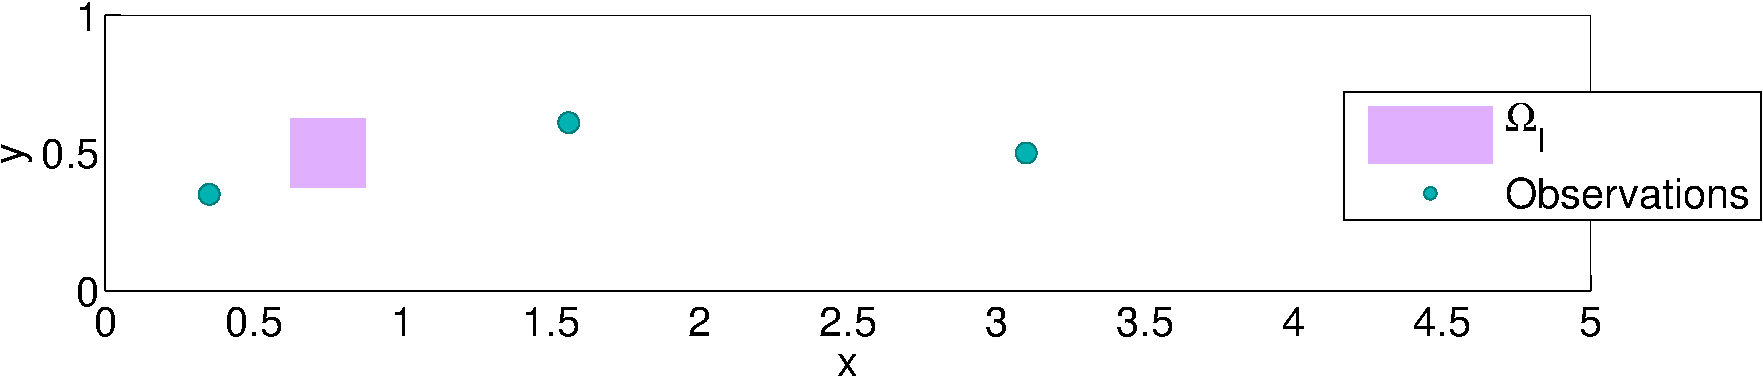
\includegraphics[width=0.8\textwidth]{baseSeries/setup_3_3.pdf}
\caption{Locations of the observations and the QoI region.}
\label{fig:baseSetup}
\end{figure}
%

For the numerical simulations, we use the finite element method (FEM), employing a continuous Galerkin formulation with Lagrange elements. We use the \texttt{libMesh} library~\cite{libMeshPaper} for the FEM calculations.
%\red{The library offers easy calculation of adjoint systems, error estimates and subdomain restricted variables.}\footnote{But we don't use Libmesh's error estimates or restrict variables to subdomains...}
The domain is discretized by a regular mesh of quadrilaterals, with 250 and 50 elements along the $x_1$ and $x_2$ directions, respectively, for a total of 12,500 elements, resulting in 12,801 degrees of freedom per variable. The diffusion coefficient is such that the cell P\'{e}clet number never exceeds 0.1, and thus no stabilization is required.

Synthetic observations consisting of the state at three points in the domain are artificially generated by running the high-fidelity model on a finer mesh with the true forcing field
%
\begin{equation}
f_{true}(x_1,x_2)=
\begin{cases}
1.0 & \textrm{if }(x_1,x_2)\in[0.125,0.375]\times[0.125,0.375] \\
0.8 & \textrm{if }(x_1,x_2)\in[2.375,2.625]\times[0.375,0.625] \\
0 & \textrm{otherwise}.
\end{cases}
\end{equation}
%
%
%------------------------------------------------------------%
\subsubsection{Adaptive Model Refinement Results} \label{sec:cdvcdrBaseRef}
%------------------------------------------------------------%
%

We now present the results for solving the inference problem using \cref{alg:refSeries}. Once the QoI error estimate is calculated using \cref{eq:finErrExp}, the error estimate is then decomposed into local contributions. At each iteration, based on this decomposition, we choose the basis functions with the largest error contributions until an additional 5\% of the elements has been marked for refinement. This is repeated until the estimated absolute relative error in the QoI, calculated as $\epsilon_i/(\epsilon_i+I(q_{MF_i},u_{MF_i}))$, is less than $1\%$.

\Cref{fig:baseRef} shows the local error contributions, as well as the subdomains where the low- and high-fidelity models are used, for the series of mixed-fidelity models thus generated. \DIFdelbegin \DIFdel{Each linear Lagrange basis function's contribution is plotted at its nonzero node.
}\DIFdelend %DIF > Each linear Lagrange basis function's contribution is plotted at its nonzero node.
%
\begin{figure}[htbp]
%\captionsetup[subfloat]{captionskip=-5pt}
\centering
\subfloat[LF $\equiv$ MF$_0$ ($0\%$ HF)]{
  \includegraphics[width=0.46\textwidth]{baseSeries/cd_cdr_LF_divvy.png}
  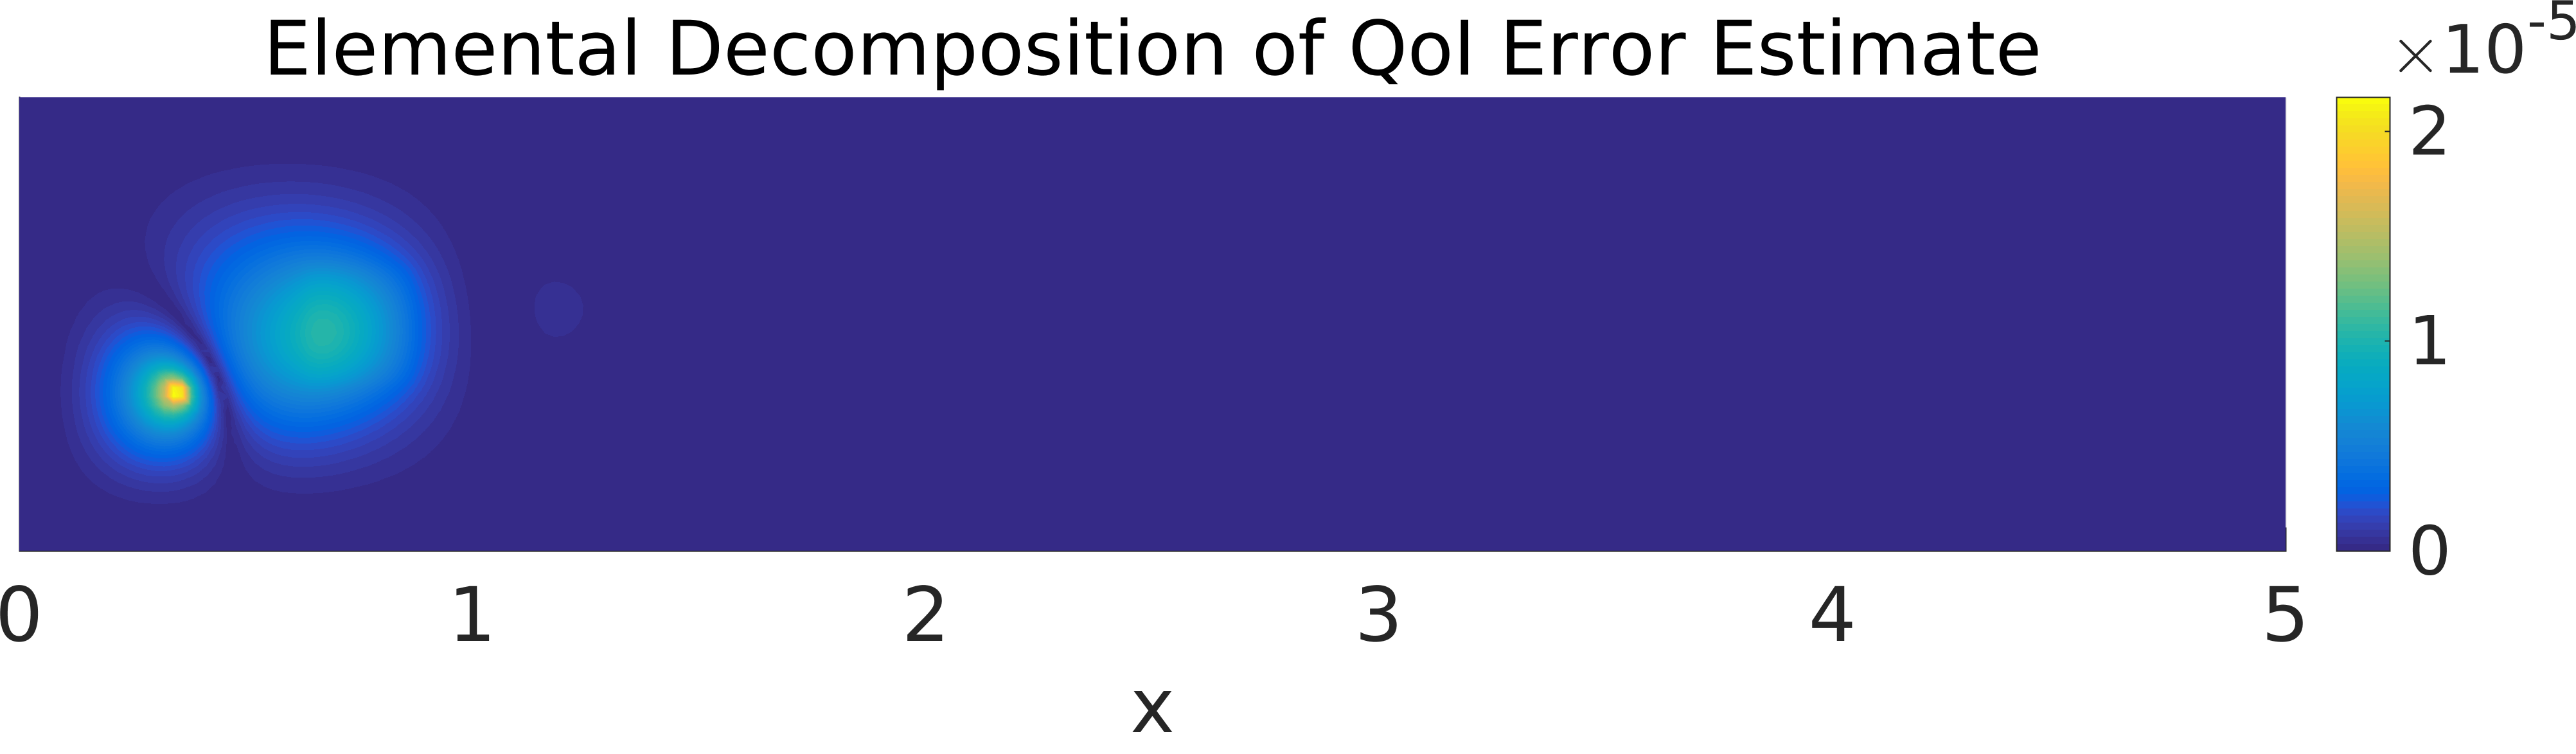
\includegraphics[width=0.49\textwidth]{baseSeries/err_breakdown_LF.png}
  \label{fig:baseRef0}
} \\
\subfloat[MF$_1$ ($5\%$ HF)]{
  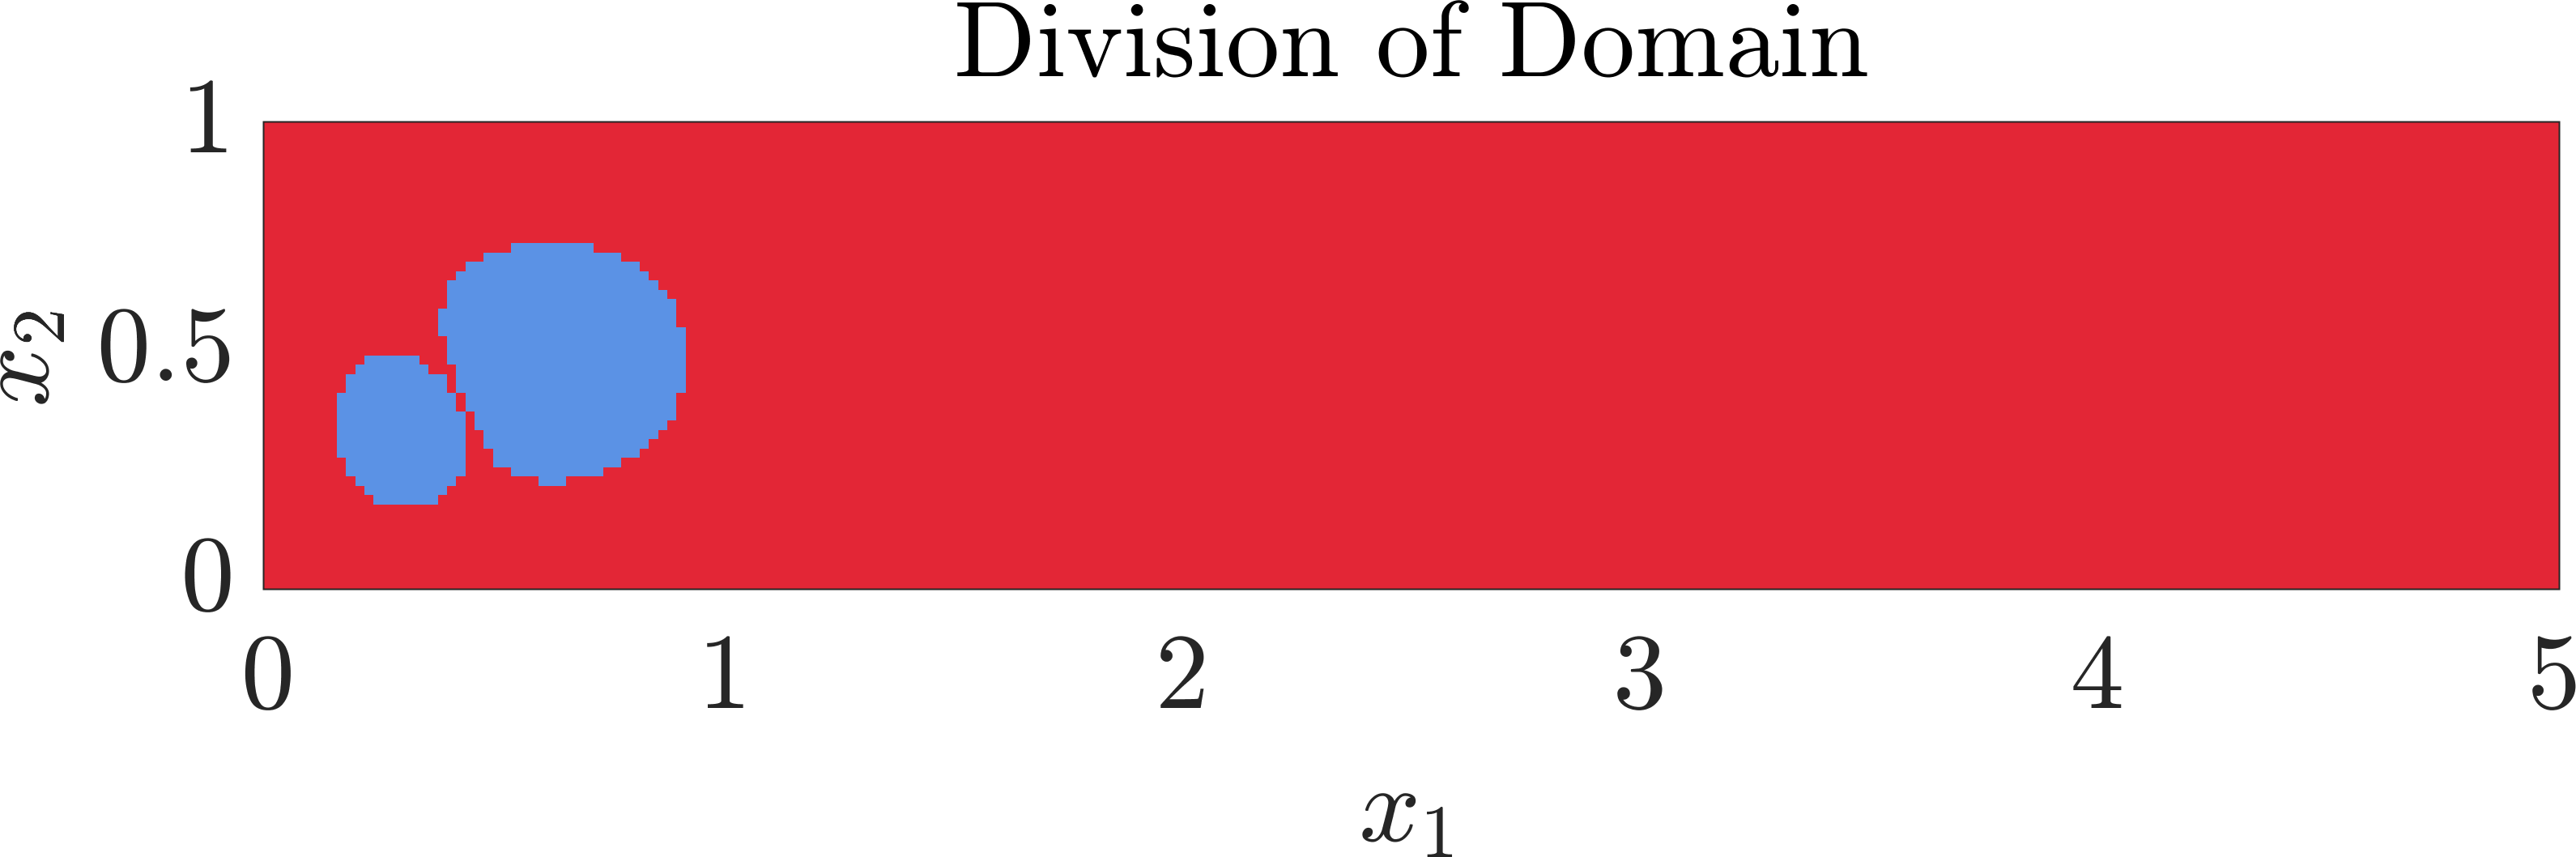
\includegraphics[width=0.46\textwidth]{baseSeries/cd_cdr_MF01_divvy.png}
  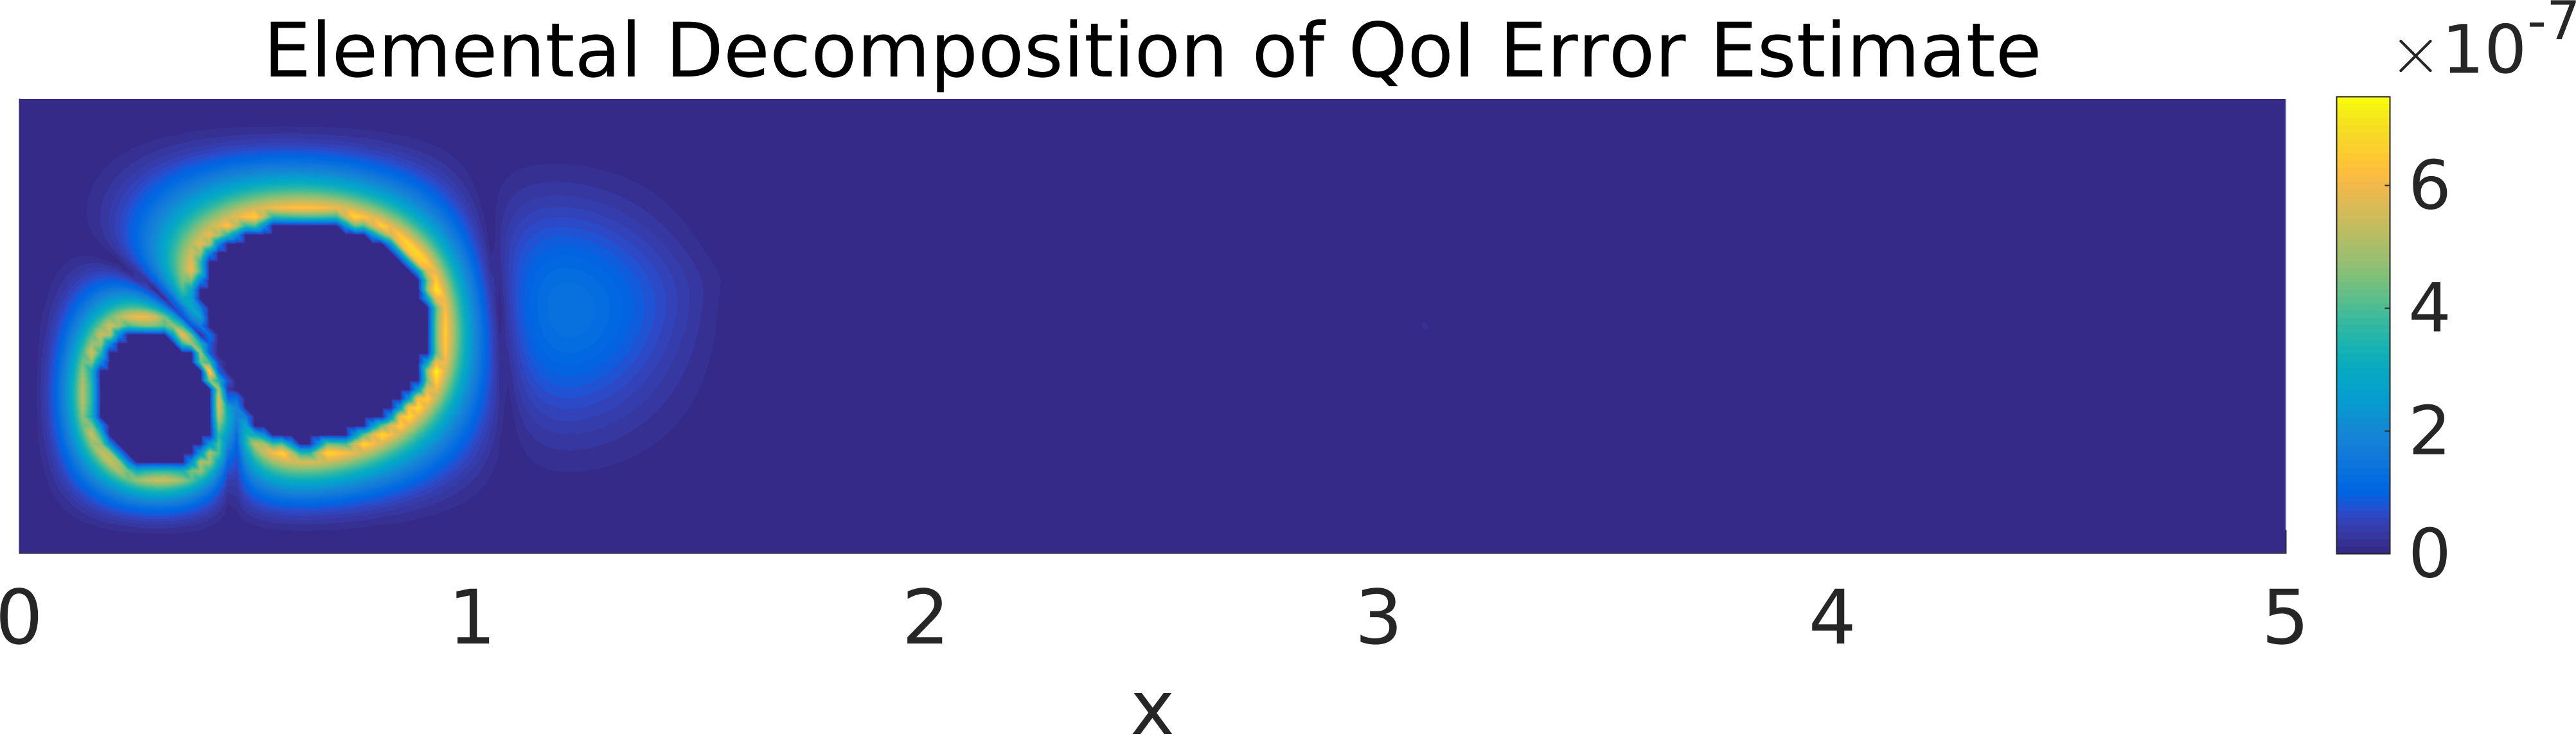
\includegraphics[width=0.49\textwidth]{baseSeries/err_breakdown_MF01.png}
} \\
\subfloat[MF$_2$ ($10\%$ HF)]{
  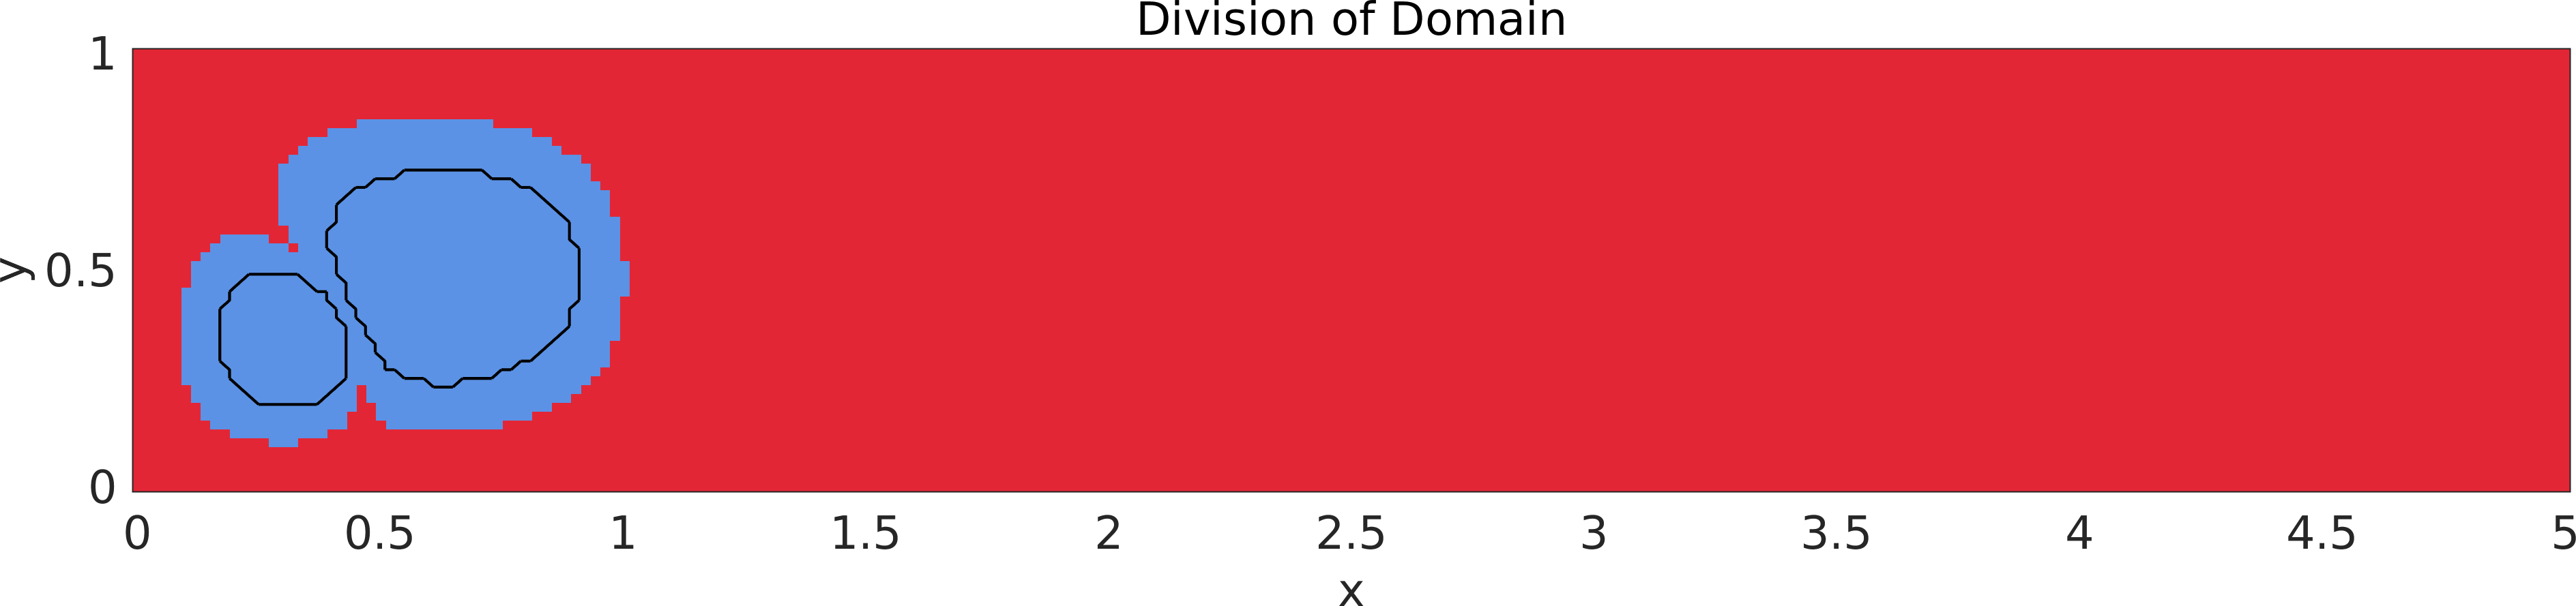
\includegraphics[width=0.46\textwidth]{baseSeries/cd_cdr_MF02_divvy.png}
  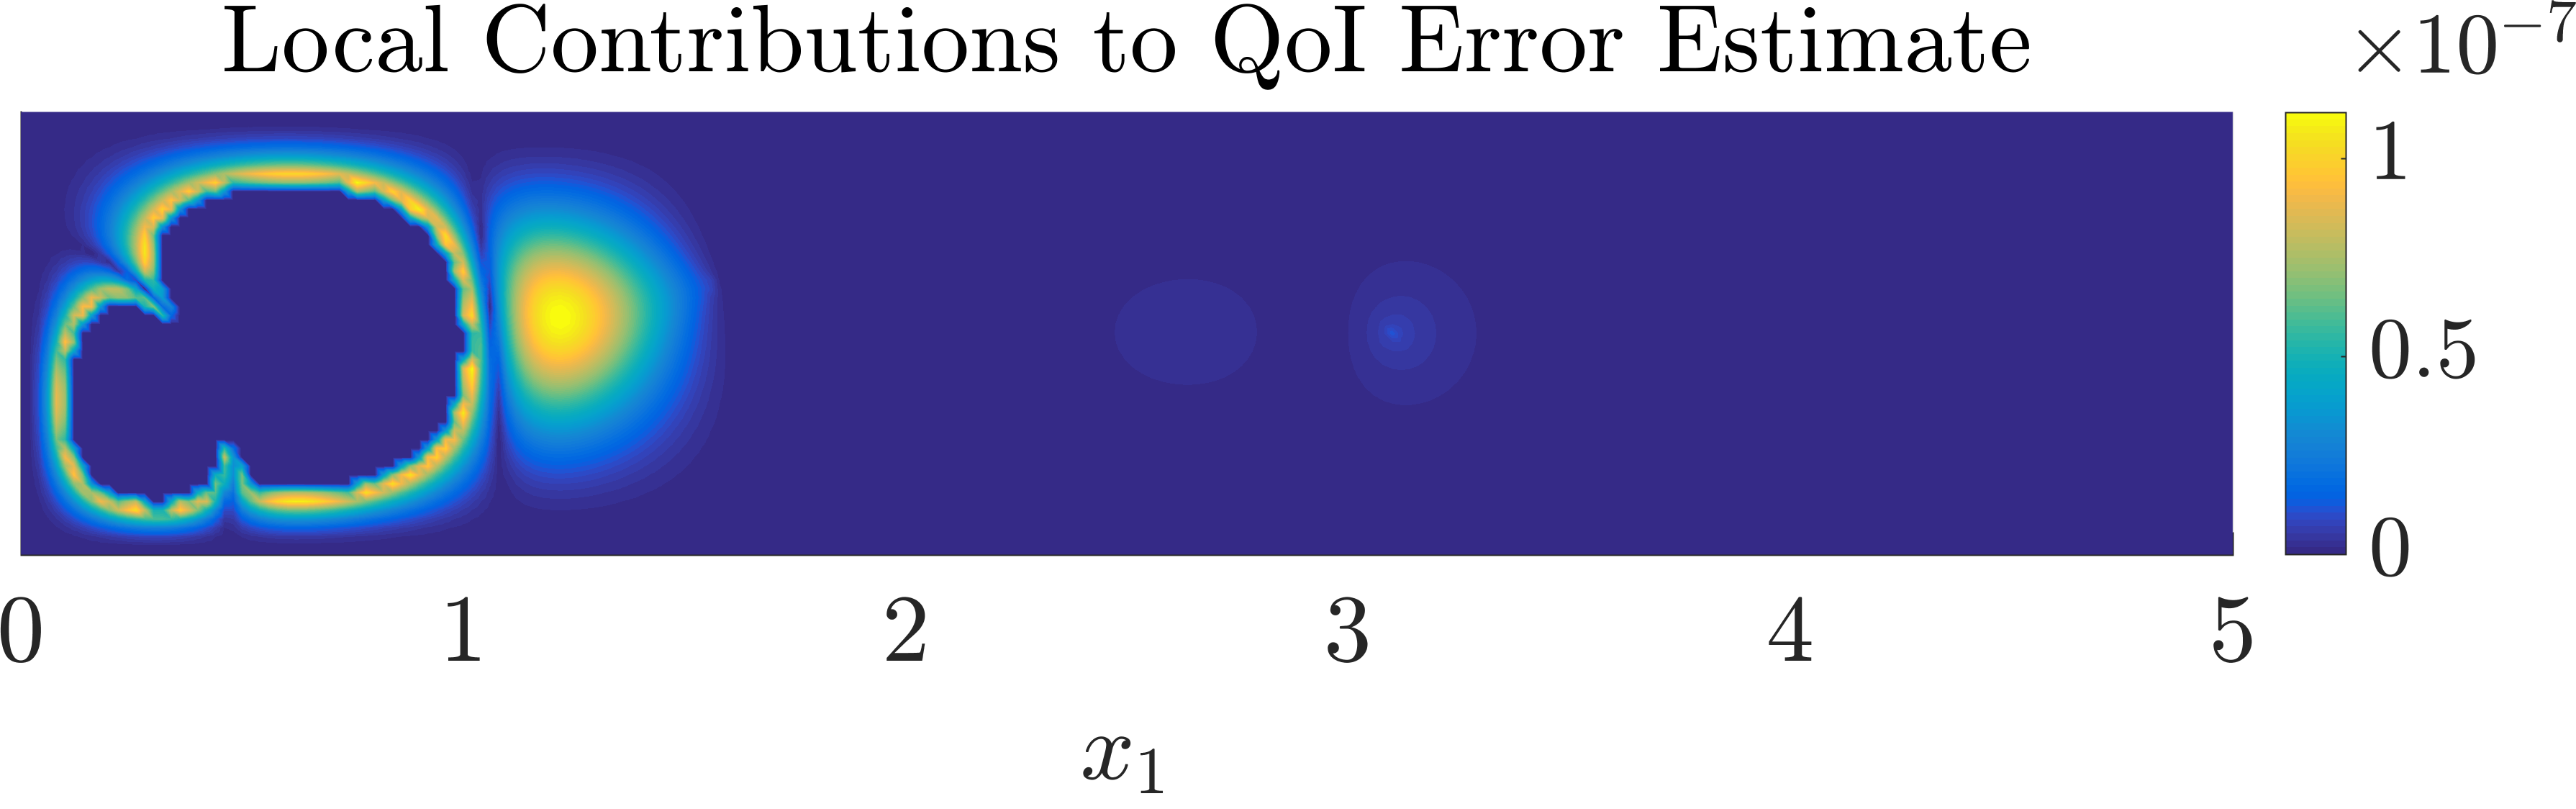
\includegraphics[width=0.49\textwidth]{baseSeries/err_breakdown_MF02.png}
} \\
\caption{Left: Multi-fidelity refinement over the domain (low-fidelity convection-diffusion model used in red portion, high-fidelity convection-diffusion-reaction model used in blue portion). Right: local error contributions. }
\label{fig:baseRef}
\end{figure}
%
Note that the error contribution of each basis function whose support is entirely within the high-fidelity regions is zero.

We see that the largest local error \DIFdelbegin \DIFdel{contribution is }\DIFdelend \DIFaddbegin \DIFadd{contributions are }\DIFaddend concentrated in the QoI region \DIFdelbegin \DIFdel{, and the data point }\DIFdelend \DIFaddbegin \DIFadd{and around the observation location }\DIFaddend closest to the QoI. %DIF <  KW: I am not sure how to read the second phrase in this first sentence. Is it '...contribution is concentrated in two places: in the QoI region and near the observation location closest to the QoI.'  ??
In the first decomposition of the error (\cref{fig:baseRef0}), the region where the elemental error is \DIFdelbegin \DIFdel{maximum is the leftmost data point. %DIF <  KW: again here, what is a 'data point' ? Do you mean 'observation location' ?
}\DIFdelend \DIFaddbegin \DIFadd{greatest is around the leftmost observation location. }\DIFaddend Since the constraining model is an elliptic PDE, with weak convection, information flow is localized, and is weakly convected from left to right. Therefore, for the calculation of the QoI, it is most important to refine the region near the leftmost \DIFdelbegin \DIFdel{data point, and }\DIFdelend \DIFaddbegin \DIFadd{observation location, and then around }\DIFaddend the QoI region. %DIF <  KW: same here. plus another confusing comma.
After that, the error decomposition suggests refinement in regions upstream and around the middle \DIFdelbegin \DIFdel{data point}\DIFdelend \DIFaddbegin \DIFadd{observation location}\DIFaddend , and then the rightmost \DIFdelbegin \DIFdel{data point.
%DIF <  KW: and here
}\DIFdelend \DIFaddbegin \DIFadd{observation location.
}\DIFaddend 

\Cref{fig:baseErr} shows the true and estimated absolute relative errors in the QoI for the various mixed-fidelity models generated by \cref{alg:refSeries}; the true and estimated relative errors are calculated relative to the true and estimated high-fidelity QoI, respectively. In this case, we see that QoI error of $1\%$ is attained with a mixed-fidelity model where the high-fidelity model is used in only about $10\%$ of the domain. We note that while here the error is seen to decrease with increasing refinement, in general there is no guarantee that either the error in the QoI or the relative error in the error estimate will decrease monotonically as more of the domain is refined.
%
\begin{figure}[htbp]
\centering
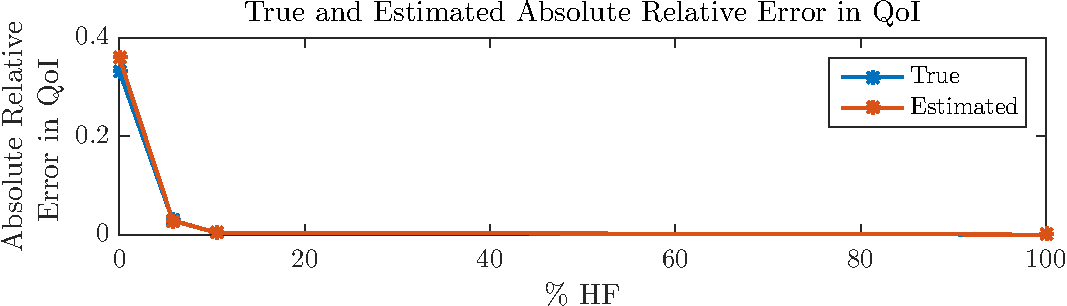
\includegraphics[width=0.8\textwidth]{baseSeries/err_est.pdf}
\caption{True and estimated absolute relative error in QoI, plotted as a function of the percentage area of the domain in which the high-fidelity convection-diffusion-reaction model is used.}
\label{fig:baseErr}
\end{figure}
%

%------------------------------------------------------------%
\subsubsection{Interaction of Observations and QoI} \label{sec:qoivdata}
%------------------------------------------------------------%
%
The error estimate decomposition suggests the use of the high-fidelity model in areas of the domain that are important to the interaction between the observations and QoI; the interaction between these two can be complex, and the areas suggested for refinement may be nonintuitive. To see this, we compare the error estimate decomposition for three sizes of the QoI region $\Omega_I$ given the same set of \DIFdelbegin \DIFdel{data points}\DIFdelend \DIFaddbegin \DIFadd{observation locations}\DIFaddend , and for three nested sets of \DIFdelbegin \DIFdel{data points }\DIFdelend \DIFaddbegin \DIFadd{observation locations }\DIFaddend given the same QoI region. For the sake of illustration, we make two refinement iterations for each combination of observations and QoI region, regardless of the magnitude of the relative error estimate. However, in conducting the numerical experiments, it was observed that the number of iterations needed to achieve a given tolerance tended to increase as the QoI region increased.

\cref{fig:qoiStudy} shows the domain for three cases considered, with the same set of observations but increasingly large, nested QoI regions $\Omega_I$.
The error decompositions for each case are also shown in \cref{fig:qoiStudy}. The bottom row gives the baseline case presented in \cref{sec:cdvcdrBaseRef}, although here we choose the basis functions $i$ whose error $\varepsilon_i$ are among the largest $5\%$, \DIFaddbegin \DIFadd{rather than only enough basis functions to cover 5\% of the domain in their support, }\DIFaddend so the proportion of \DIFdelbegin \DIFdel{additional refined elements }\DIFdelend \DIFaddbegin \DIFadd{elements marked for refinement }\DIFaddend in each iteration \DIFdelbegin \DIFdel{is slightly larger }\DIFdelend \DIFaddbegin \DIFadd{will be slightly larger than in }\cref{sec:cdvcdrBaseRef}\DIFaddend .
% KW: I don't understand this last sentence. What's the difference with Section 4.1.2?
Although refinement is still most important around the \DIFdelbegin \DIFdel{data point }\DIFdelend \DIFaddbegin \DIFadd{observation location }\DIFaddend closest to $x_1=0$, as the QoI region expands the other two \DIFdelbegin \DIFdel{data points }\DIFdelend \DIFaddbegin \DIFadd{observation locations }\DIFaddend become more important in that the error decomposition suggests refinement around them earlier. As the QoI region expands, it is also more clearly noticeable that refinement is not equally important in all parts of the QoI region.
%DIF <  KW: fix references to 'data point' throughout.

\begin{figure}[htbp]
\centering
\DIFdelbeginFL %DIFDELCMD < \subfloat[Locations of observations and QoI region $\Omega_I$][Locations of \\observations and \\QoI region $\Omega_I$]{
%DIFDELCMD <   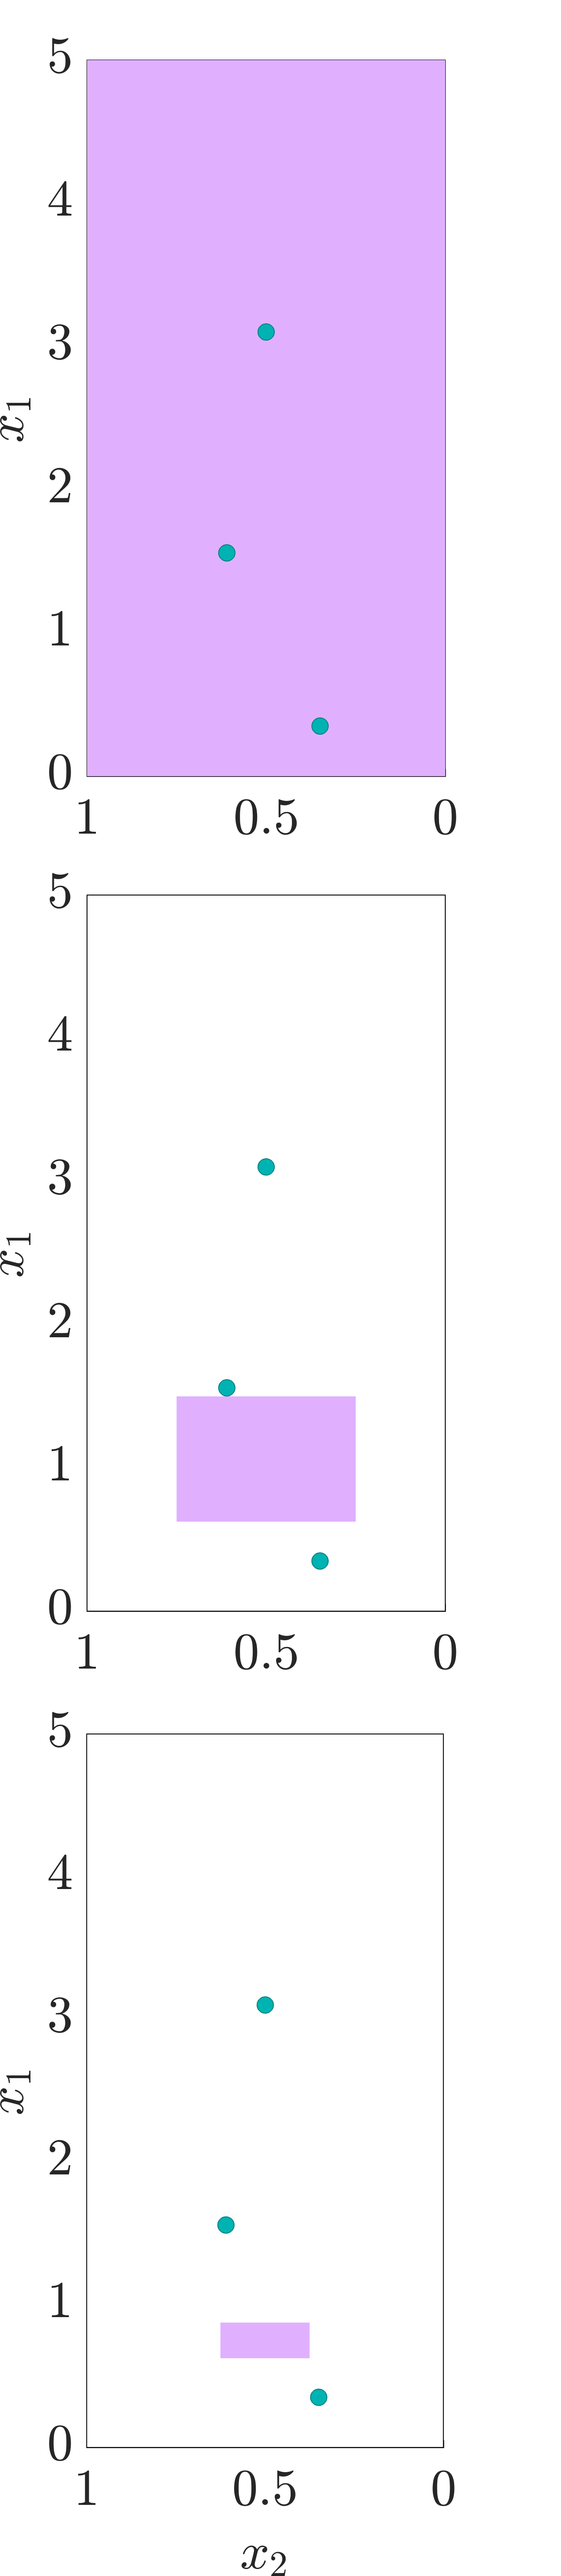
\includegraphics[width=0.23\textwidth]{vs_qoi/vs_qoi_setup.png}
%DIFDELCMD <   %DIFDELCMD < \label{subfig:obsSetup}%%%
%DIFDELCMD < }
%DIFDELCMD < \subfloat[MF$_0$ ($0\%$ HF)][MF$_0$ \\($0\%$ HF)]{
%DIFDELCMD <   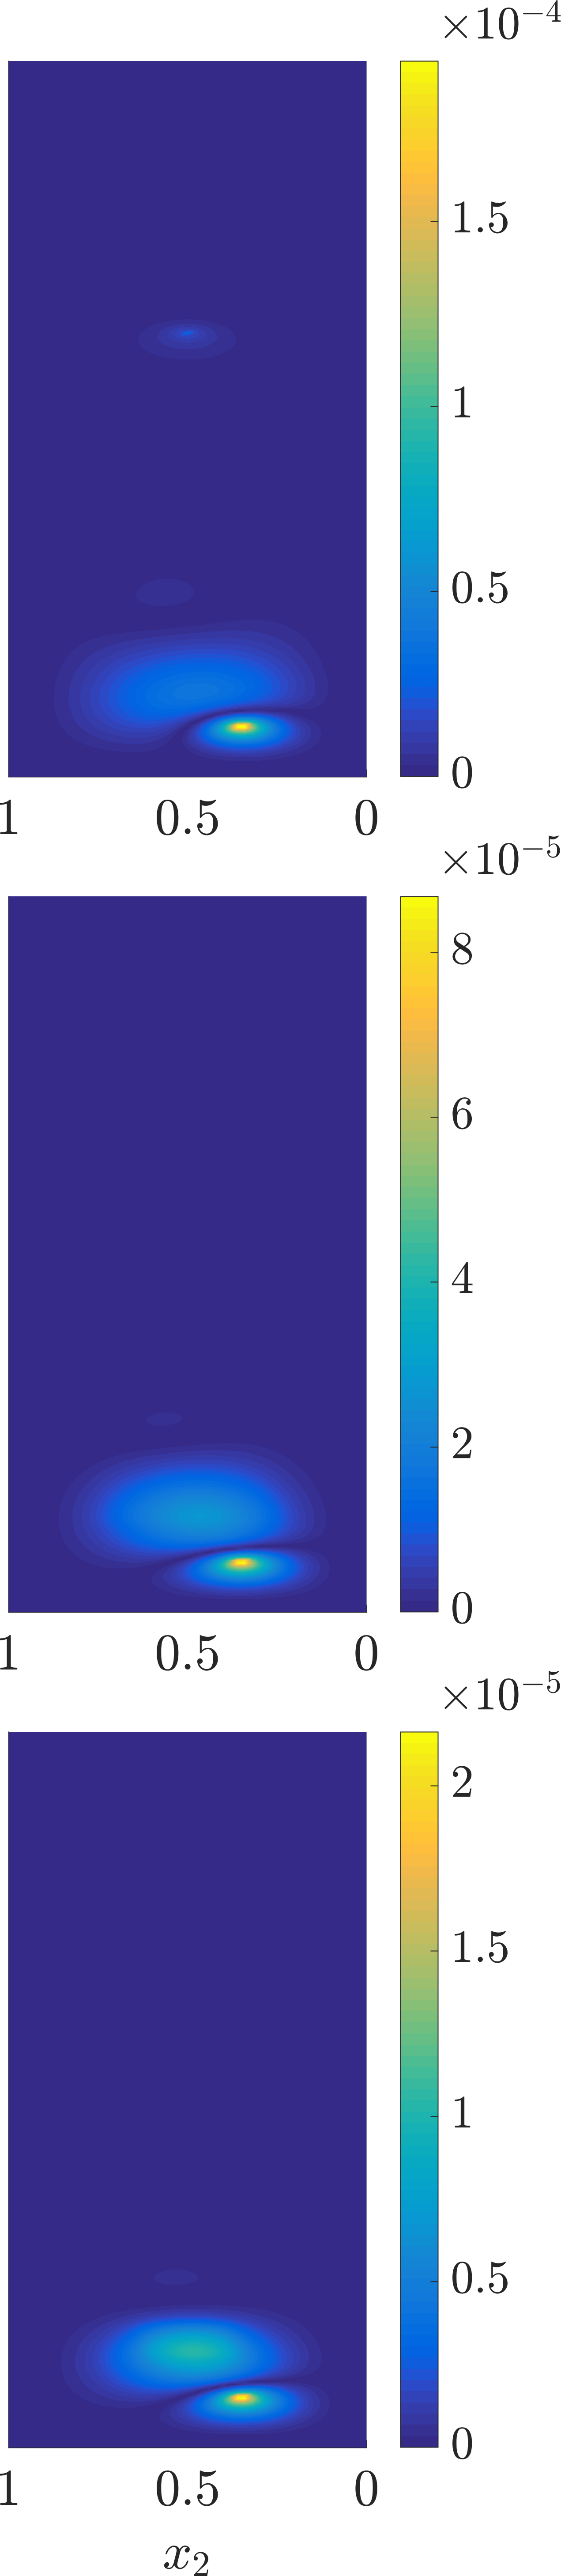
\includegraphics[width=0.23\textwidth]{vs_qoi/vs_qoi_err0.png}
%DIFDELCMD <   %DIFDELCMD < \label{subfig:obsLF}%%%
%DIFDELCMD < }
%DIFDELCMD < \subfloat[MF$_1$ ($\sim5\%$ HF)][MF$_1$ \\($\sim5\%$ HF)]{
%DIFDELCMD <   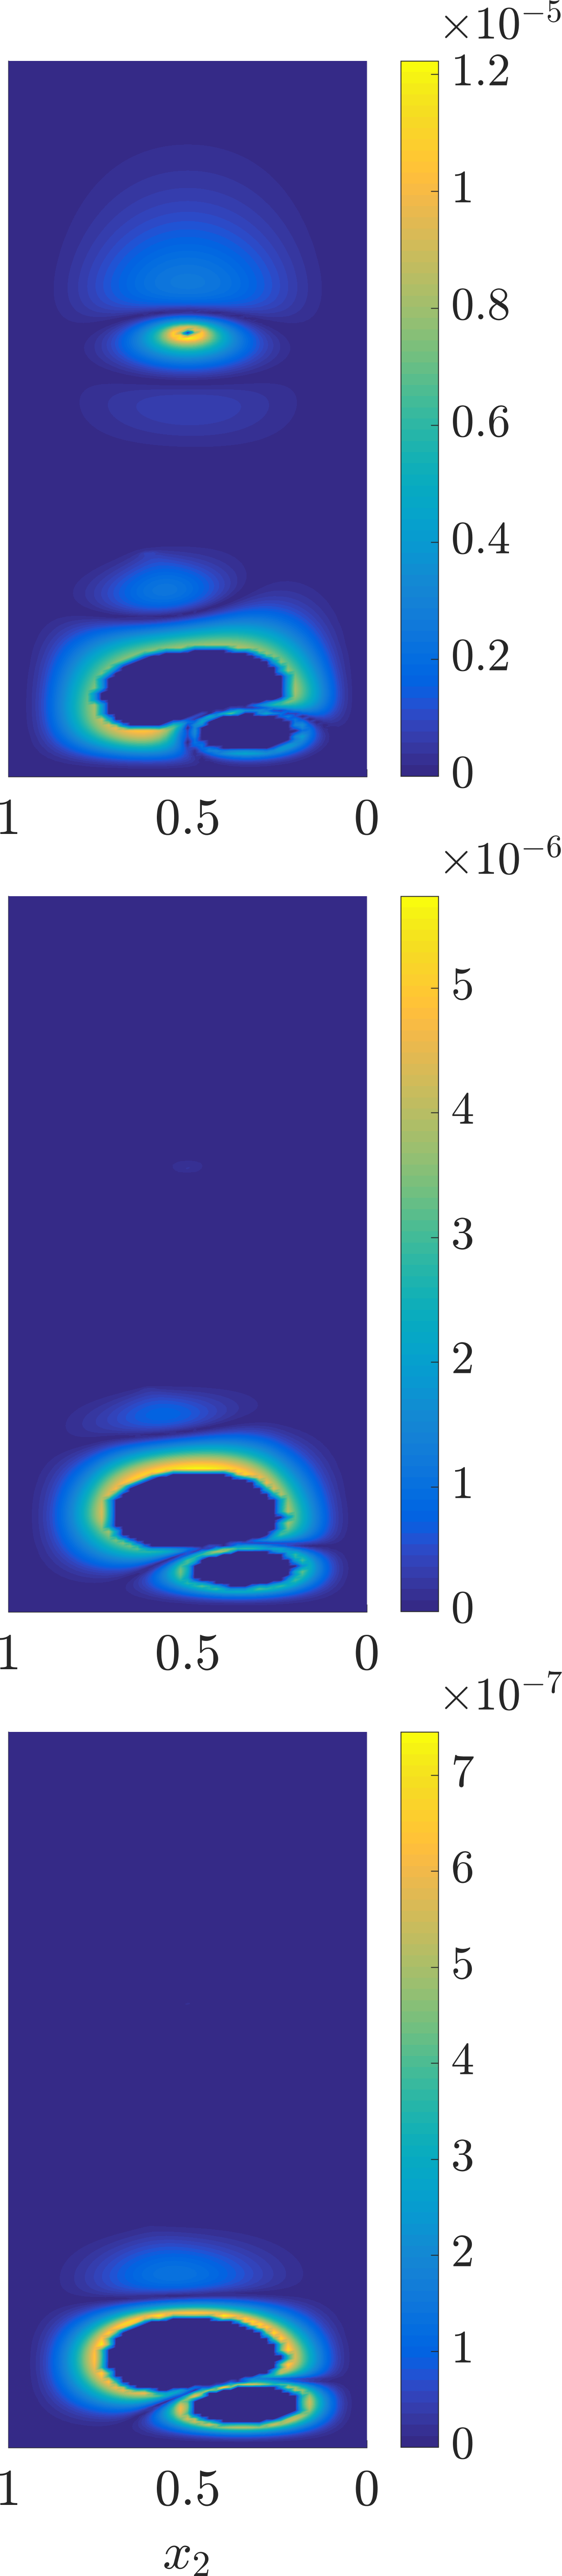
\includegraphics[width=0.23\textwidth]{vs_qoi/vs_qoi_err1.png}
%DIFDELCMD < }
%DIFDELCMD < \subfloat[MF$_2$ ($\sim10\%$ HF)][MF$_2$ \\($\sim10\%$ HF)]{
%DIFDELCMD <   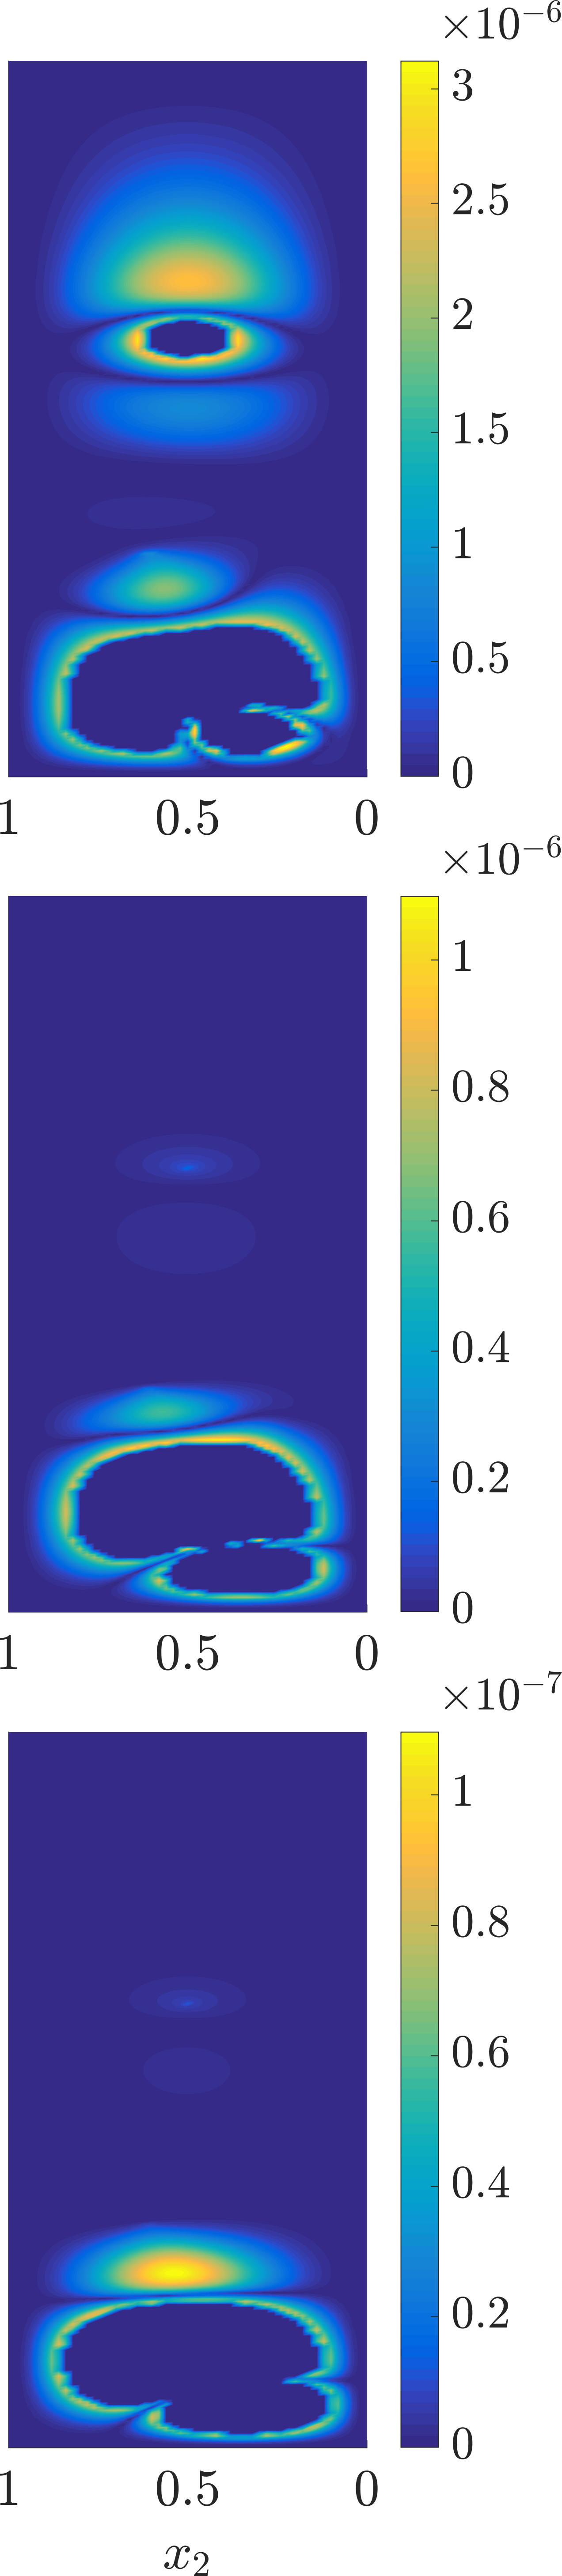
\includegraphics[width=0.23\textwidth]{vs_qoi/vs_qoi_err2.png}
%DIFDELCMD <   %DIFDELCMD < \label{subfig:obsMFlast}%%%
%DIFDELCMD < }
%DIFDELCMD <   %%%
\DIFdelendFL \DIFaddbeginFL \captionsetup{justification=centering}
\subfloat[Locations of observations and QoI region $\Omega_I$][Locations of \\observations and \\QoI region $\Omega_I$]{
  %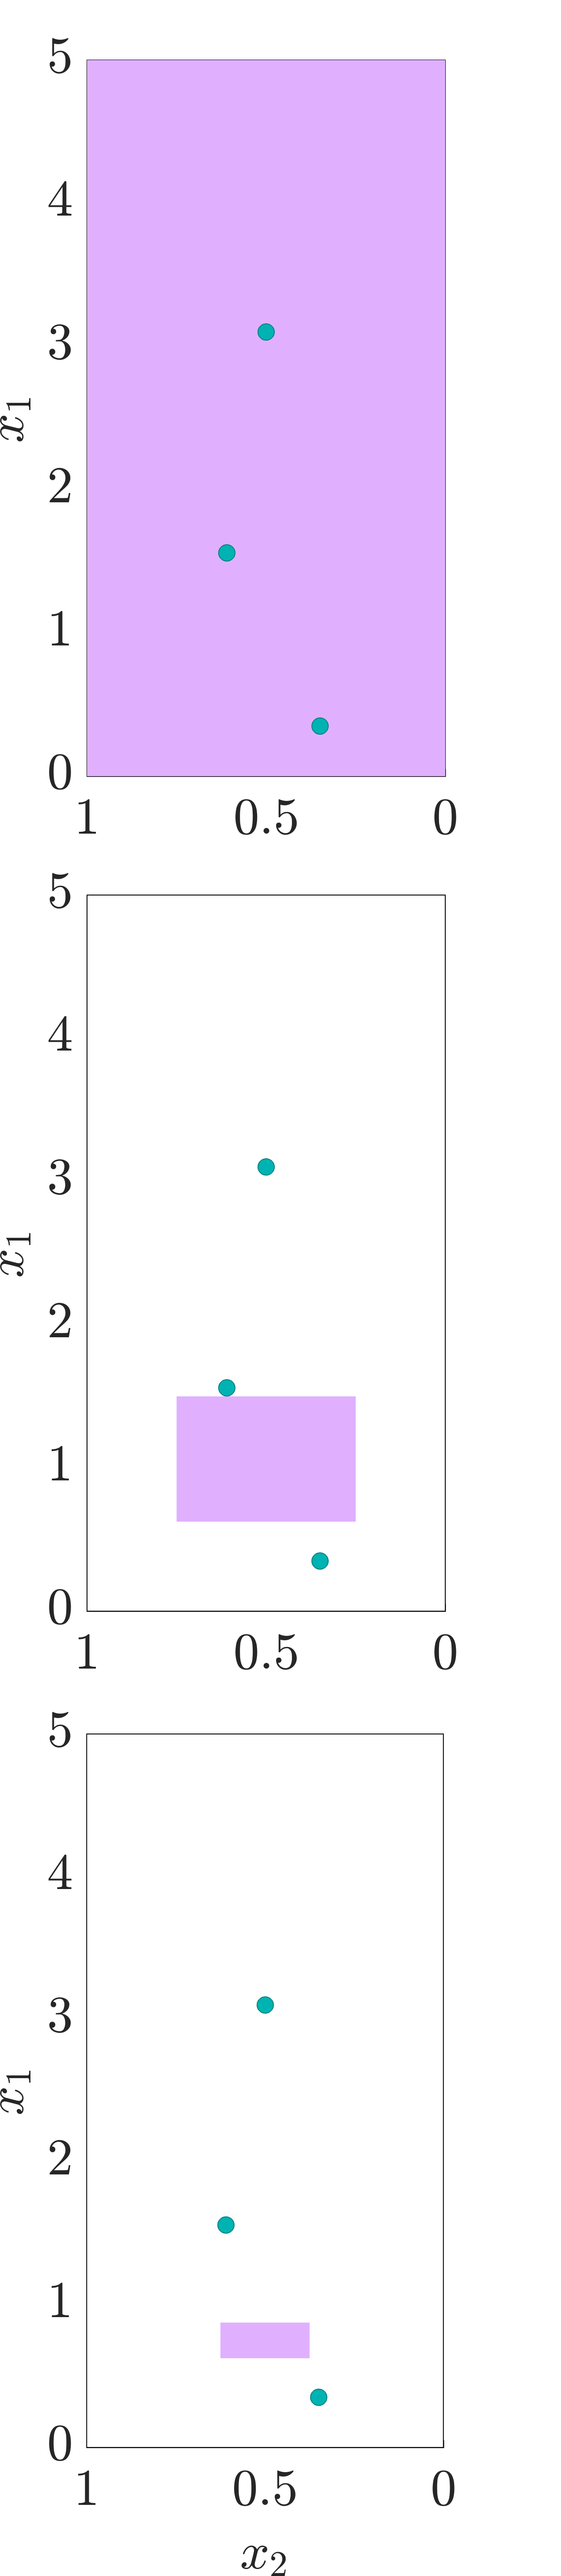
\includegraphics[width=0.23\textwidth]{vs_qoi/vs_qoi_setup.png}
  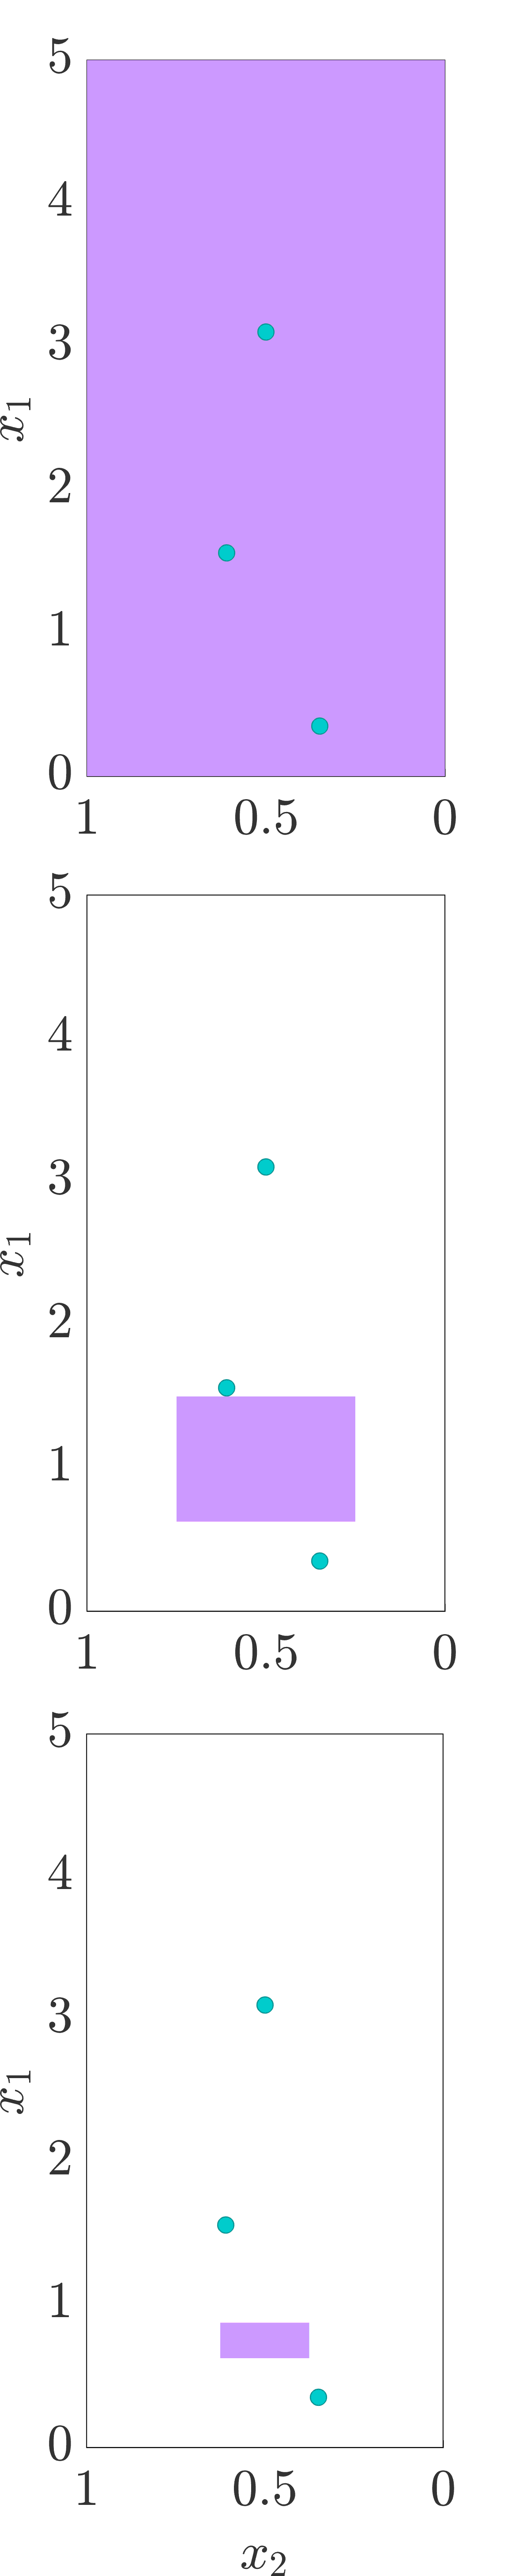
\includegraphics[width=0.21\textwidth]{vs_qoi/vs_qoi_setup_sidetrim.png}
  \label{subfig:obsSetup}
}
\captionsetup{justification=centering}
\subfloat[MF$_0$ ($0\%$ HF)][MF$_0$ \\($0\%$ HF)]{
  %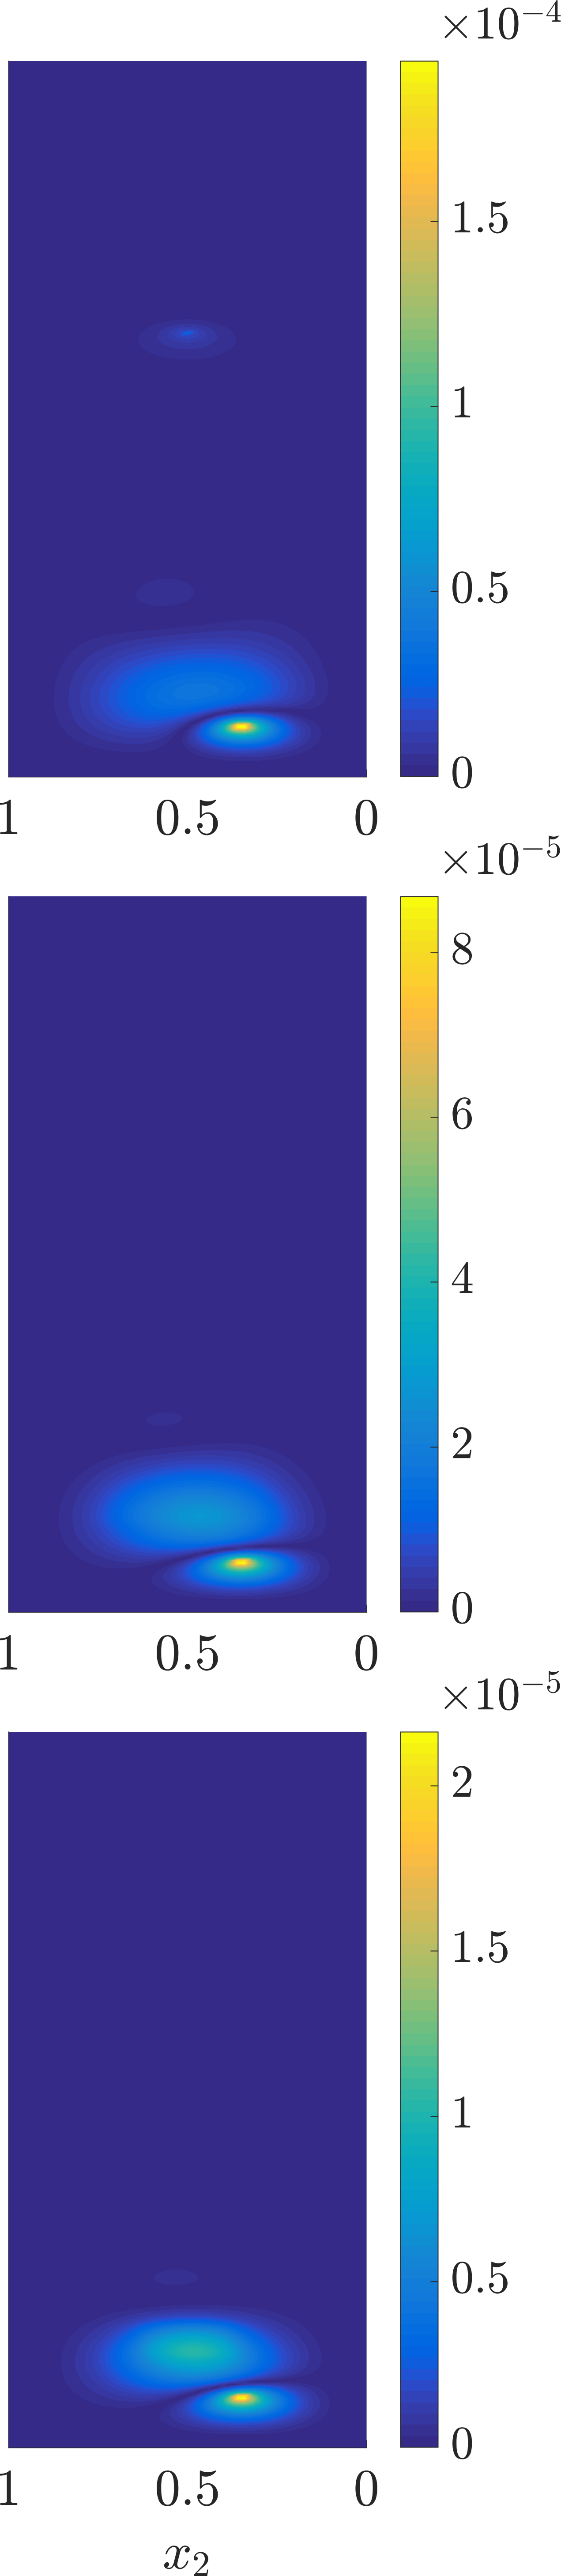
\includegraphics[width=0.23\textwidth]{vs_qoi/vs_qoi_err0.png}
  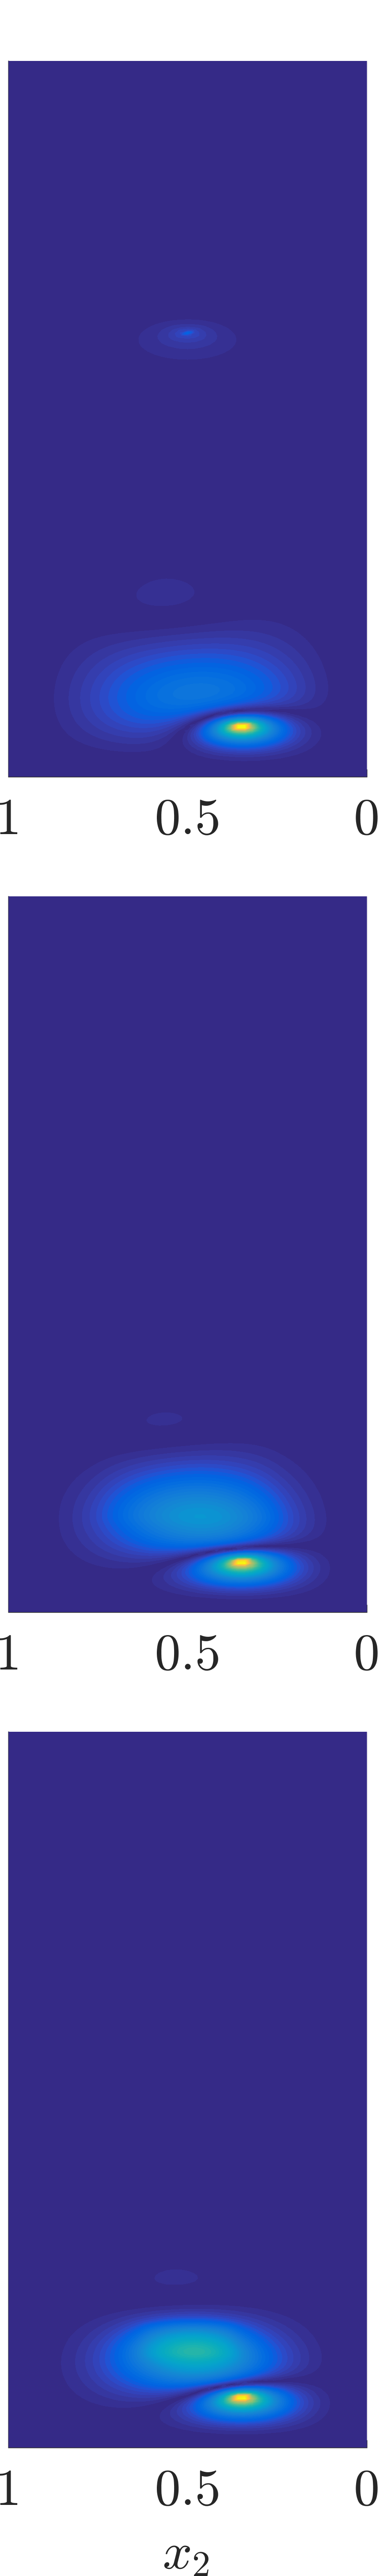
\includegraphics[width=0.16\textwidth]{vs_qoi/vs_qoi_err0_nobar.png}
  \label{subfig:obsLF}
}
\captionsetup{justification=centering}
\subfloat[MF$_1$ ($\sim5\%$ HF)][MF$_1$ \\($\sim5\%$ HF)]{
  %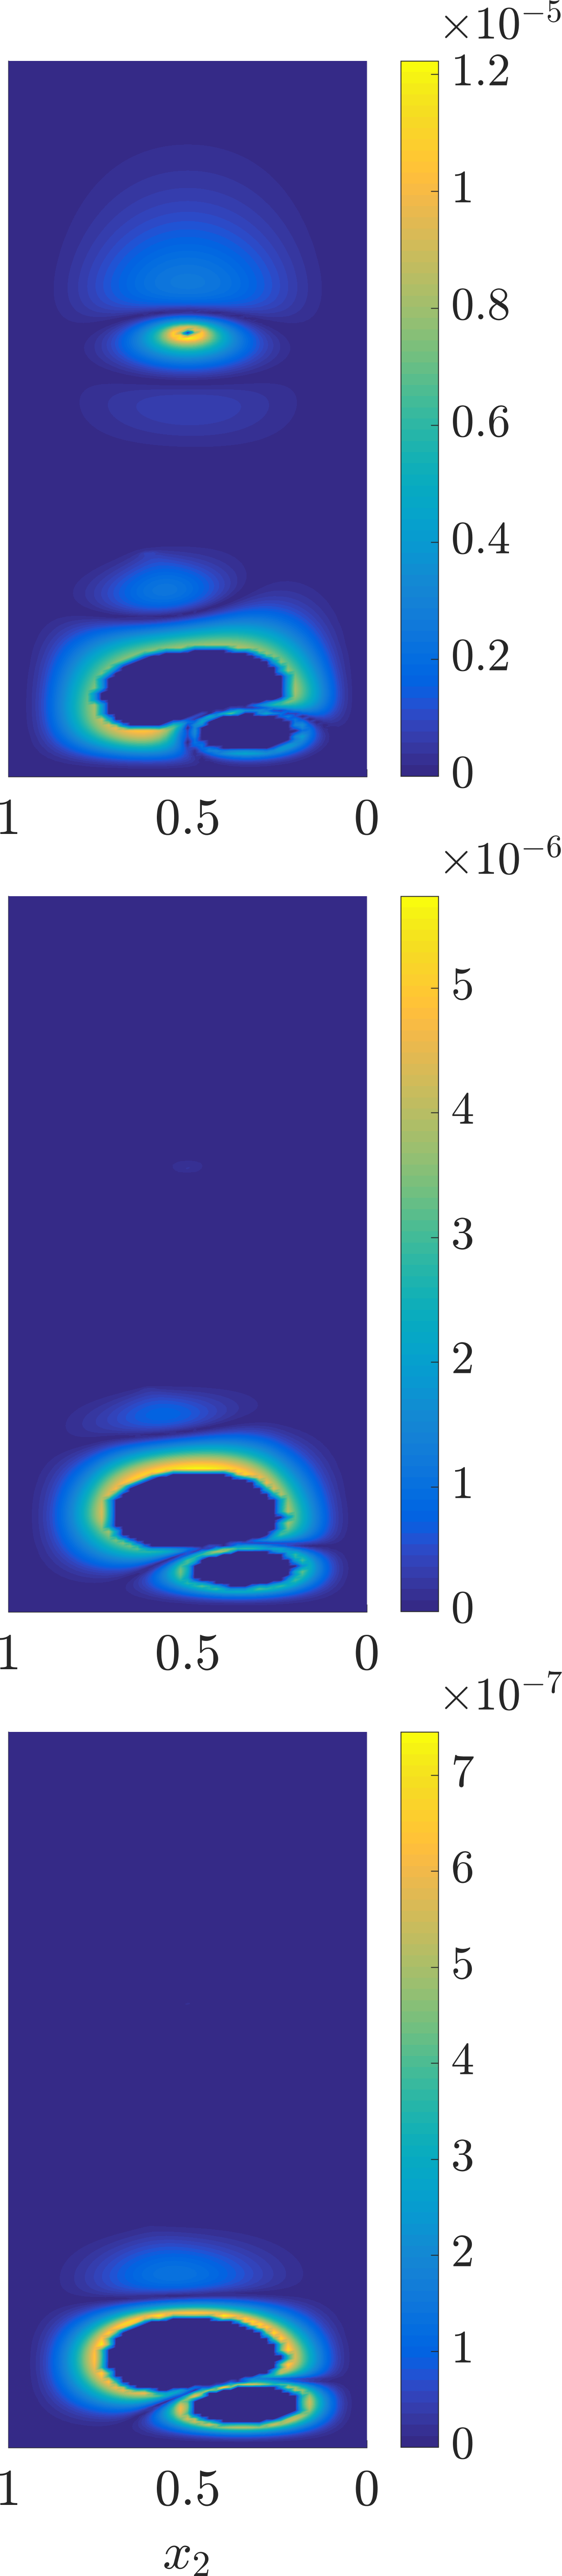
\includegraphics[width=0.23\textwidth]{vs_qoi/vs_qoi_err1.png}
  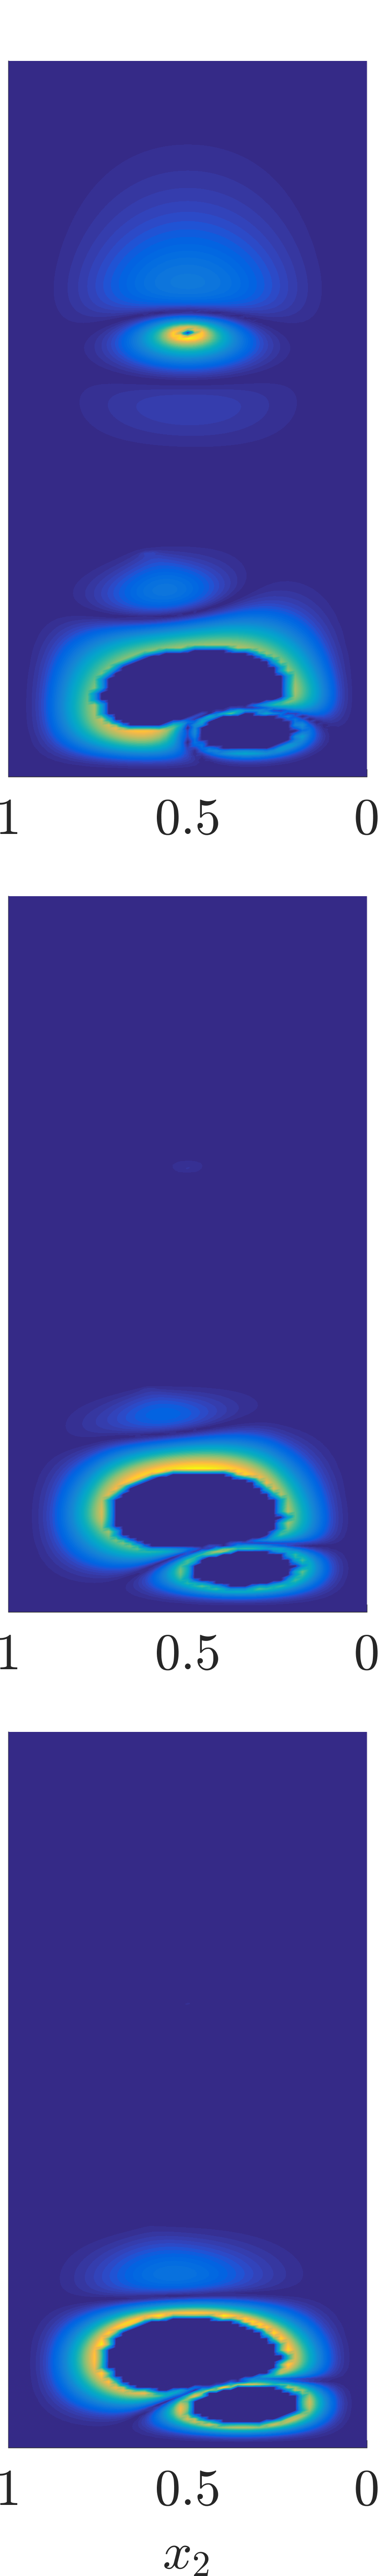
\includegraphics[width=0.16\textwidth]{vs_qoi/vs_qoi_err1_nobar.png}
}
\captionsetup{justification=centering}
\subfloat[MF$_2$ ($\sim10\%$ HF)][MF$_2$ \\($\sim10\%$ HF)]{
  %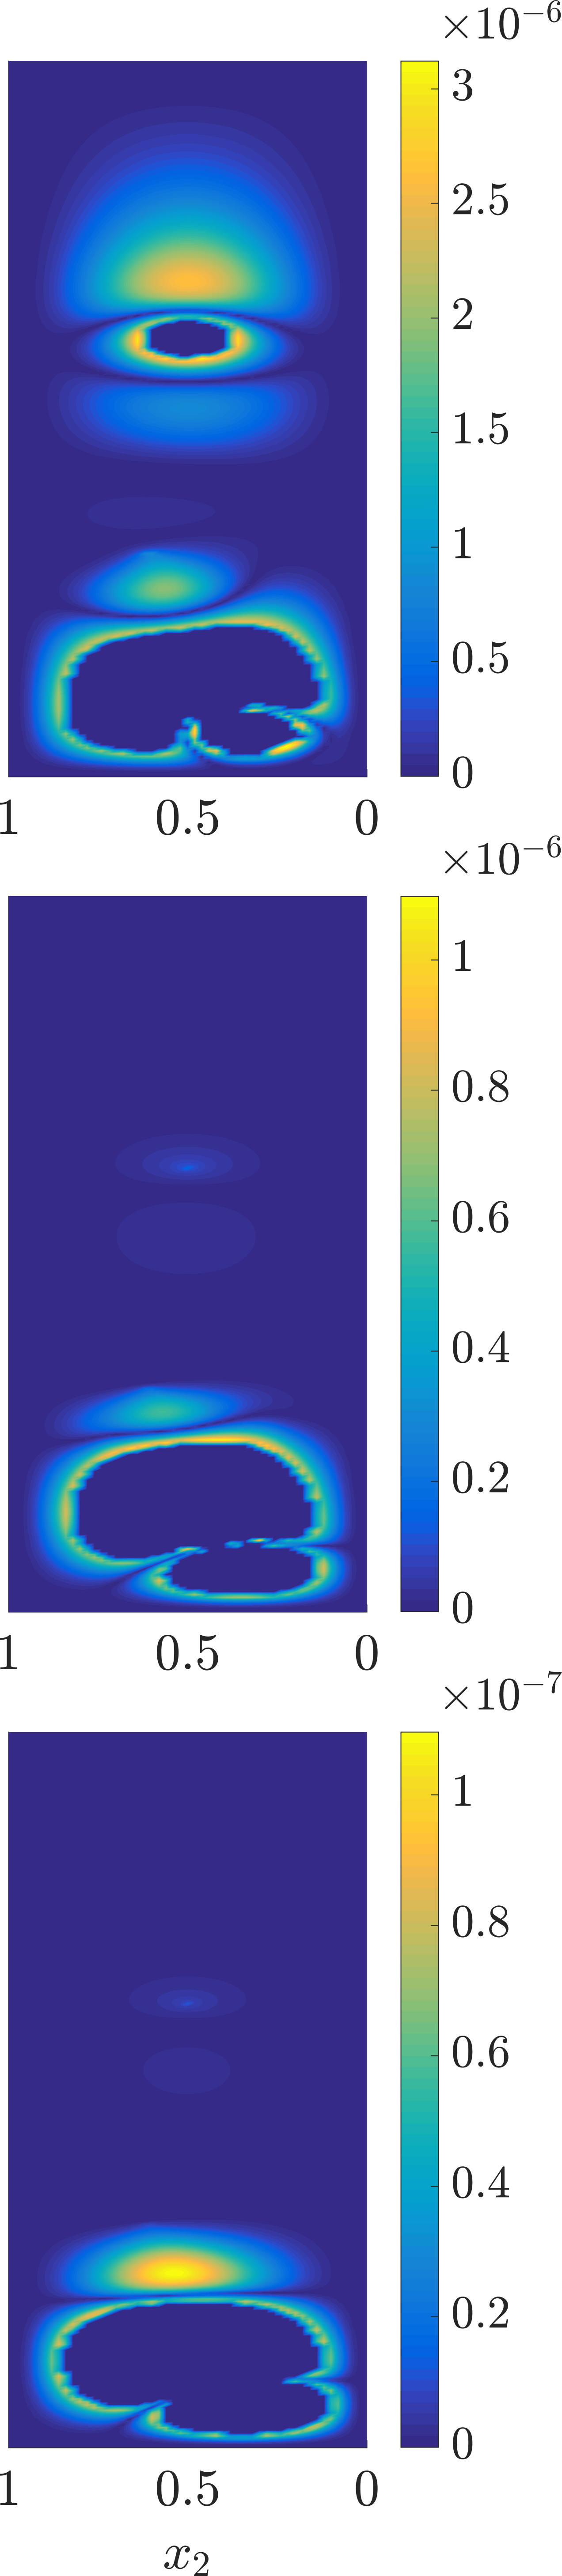
\includegraphics[width=0.23\textwidth]{vs_qoi/vs_qoi_err2.png}
  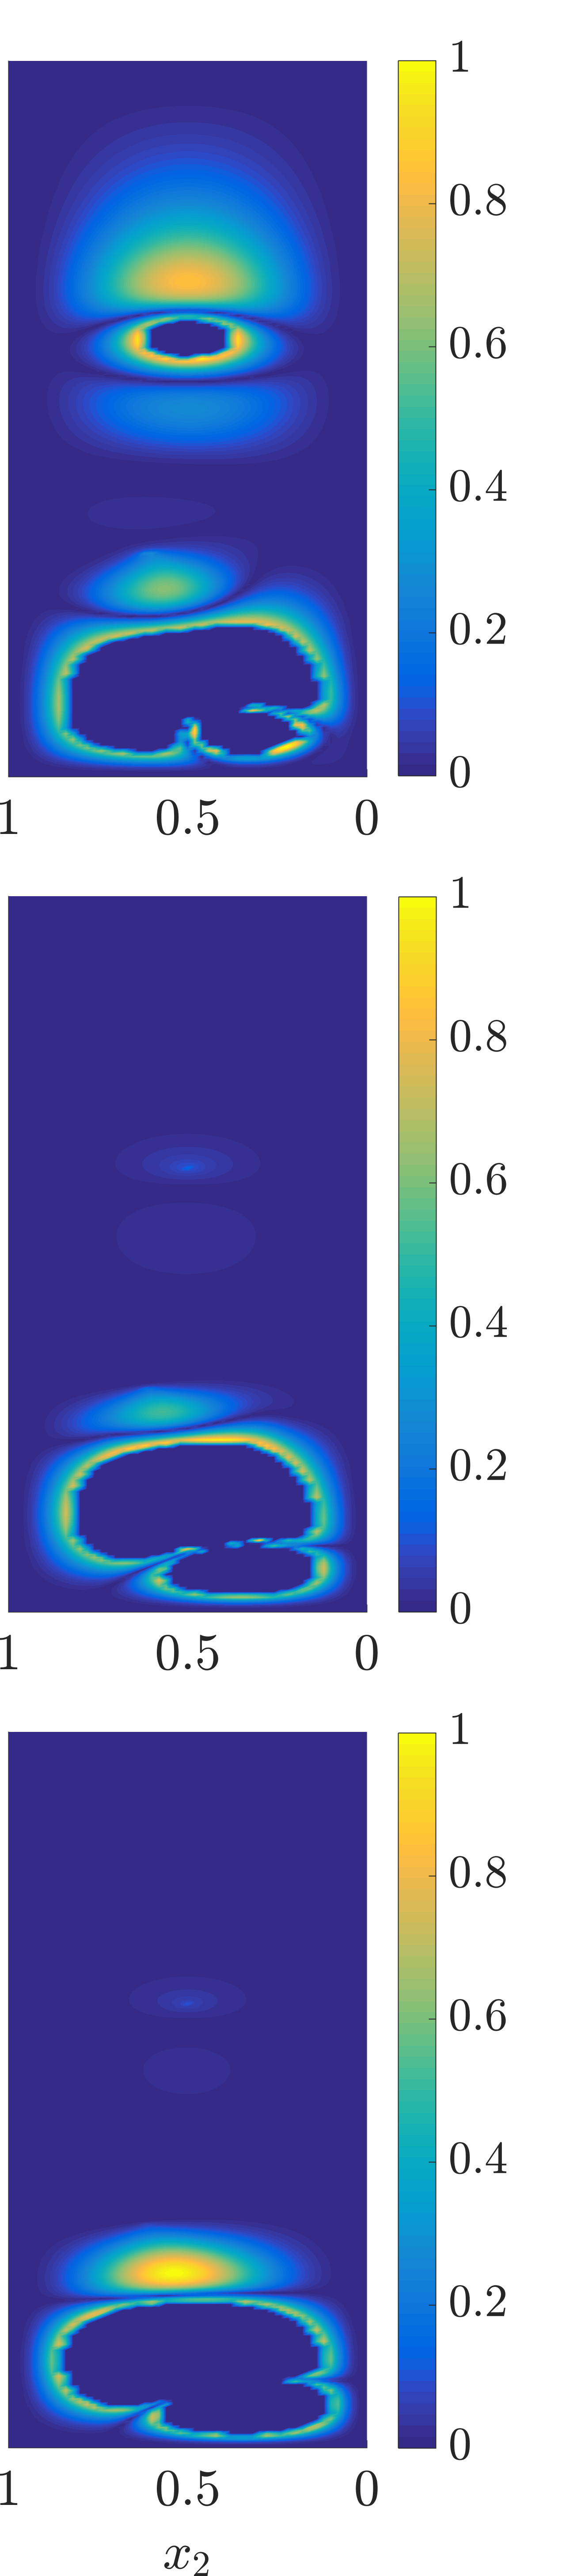
\includegraphics[width=0.23\textwidth]{vs_qoi/vs_qoi_err2_barnorm.png}
  \label{subfig:obsMFlast}
}
  \DIFaddendFL \caption{Effects of increasing the QoI region. Column \protect\DIFdelbeginFL %DIFDELCMD < \subref{subfig:obsSetup2}%%%
\DIFdelendFL \DIFaddbeginFL \protect\subref{subfig:obsSetup}\DIFaddendFL : configuration of observations (teal points) and QoI region (purple box). Columns \protect\DIFdelbeginFL %DIFDELCMD < \subref{subfig:obsLF2}%%%
\DIFdelendFL \DIFaddbeginFL \protect\subref{subfig:obsLF}\DIFaddendFL --\protect\DIFdelbeginFL %DIFDELCMD < \subref{subfig:obsMFlast2}%%%
\DIFdelendFL \DIFaddbeginFL \protect\subref{subfig:obsMFlast}\DIFaddendFL ): the \DIFaddbeginFL \DIFaddFL{relative }\DIFaddendFL error estimate decompositions for different mixed-fidelity models\DIFaddbeginFL \DIFaddFL{, relative to the largest localized error contribution; note the locations of regions of relatively large error compared to the observation locations and QoI region}\DIFaddendFL .}
  \label{fig:qoiStudy}
\end{figure}

\cref{fig:dataStudy} shows another set of cases considered, now with the same QoI region $\Omega_I$ but with increasing, nested sets of observations.
The error decomposition for the three cases is shown in \cref{fig:dataStudy}. \DIFdelbegin \DIFdel{Again, the bottom row gives the baseline case presented in }%DIFDELCMD < \cref{sec:cdvcdrBaseRef}%%%
\DIFdel{, although here the basis functions with the largest $5\%$ of the error are chosen, so the proportion of additional refined elements in each iteration is slightly larger}\DIFdelend \DIFaddbegin \DIFadd{The bottom row is the same as that in }\cref{fig:qoiStudy}\DIFaddend . Refinement appears to be consistently most important around the \DIFdelbegin \DIFdel{data point }\DIFdelend \DIFaddbegin \DIFadd{observation location }\DIFaddend closest to $x_1=0$ and the QoI region. However, as more \DIFdelbegin \DIFdel{data points }\DIFdelend \DIFaddbegin \DIFadd{observation locations }\DIFaddend are added, it becomes no longer necessarily true that refinement becomes less important around \DIFdelbegin \DIFdel{data points }\DIFdelend \DIFaddbegin \DIFadd{observation locations }\DIFaddend as their distance from the QoI region increases. \DIFdelbegin \DIFdel{The data points also interact with each other in that placing data points in regions of previously relatively uniform error contribution tends to result in a new error decomposition that is positive or negative around the data points, with valleys of zero magnitude in between }\DIFdelend \DIFaddbegin \DIFadd{In the second and third rows, one can see that after the areas around the QoI region and the two closest observation locations have been refined, the next area to be refined is not around the third closest observation location, but rather around one near the middle of the domain. This suggests that interactions between observation locations and the QoI may be non-intuitive, and in these cases a rigorous method for forming a mixed-fidelity model would be most helpful}\DIFaddend . % KW: I don't understand a lot of this discussion. You need to explain to me what you mean.

\begin{figure}[htbp]
\centering
\DIFdelbeginFL %DIFDELCMD < \subfloat[Locations of observations and QoI region $\Omega_I$][Locations of \\observations and \\QoI region $\Omega_I$]{
%DIFDELCMD <   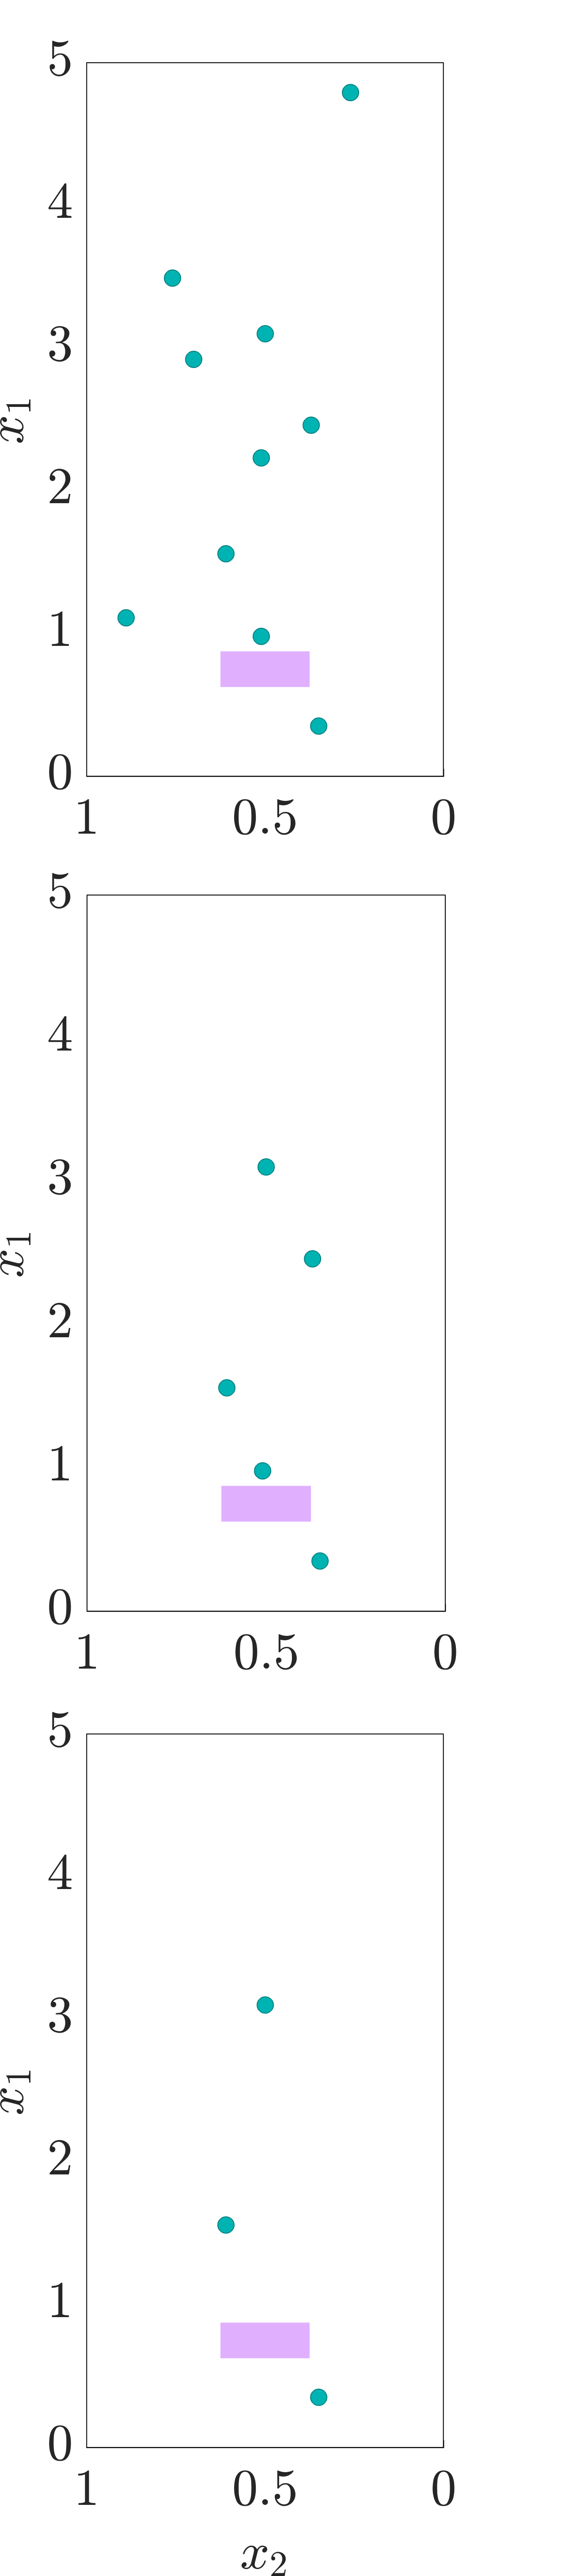
\includegraphics[width=0.23\textwidth]{vs_data/vs_data_setup.png}
%DIFDELCMD <   %DIFDELCMD < \label{subfig:obsSetup2}%%%
%DIFDELCMD < }
%DIFDELCMD < \subfloat[MF$_0$ ($0\%$ HF)][MF$_0$ \\($0\%$ HF)]{
%DIFDELCMD <   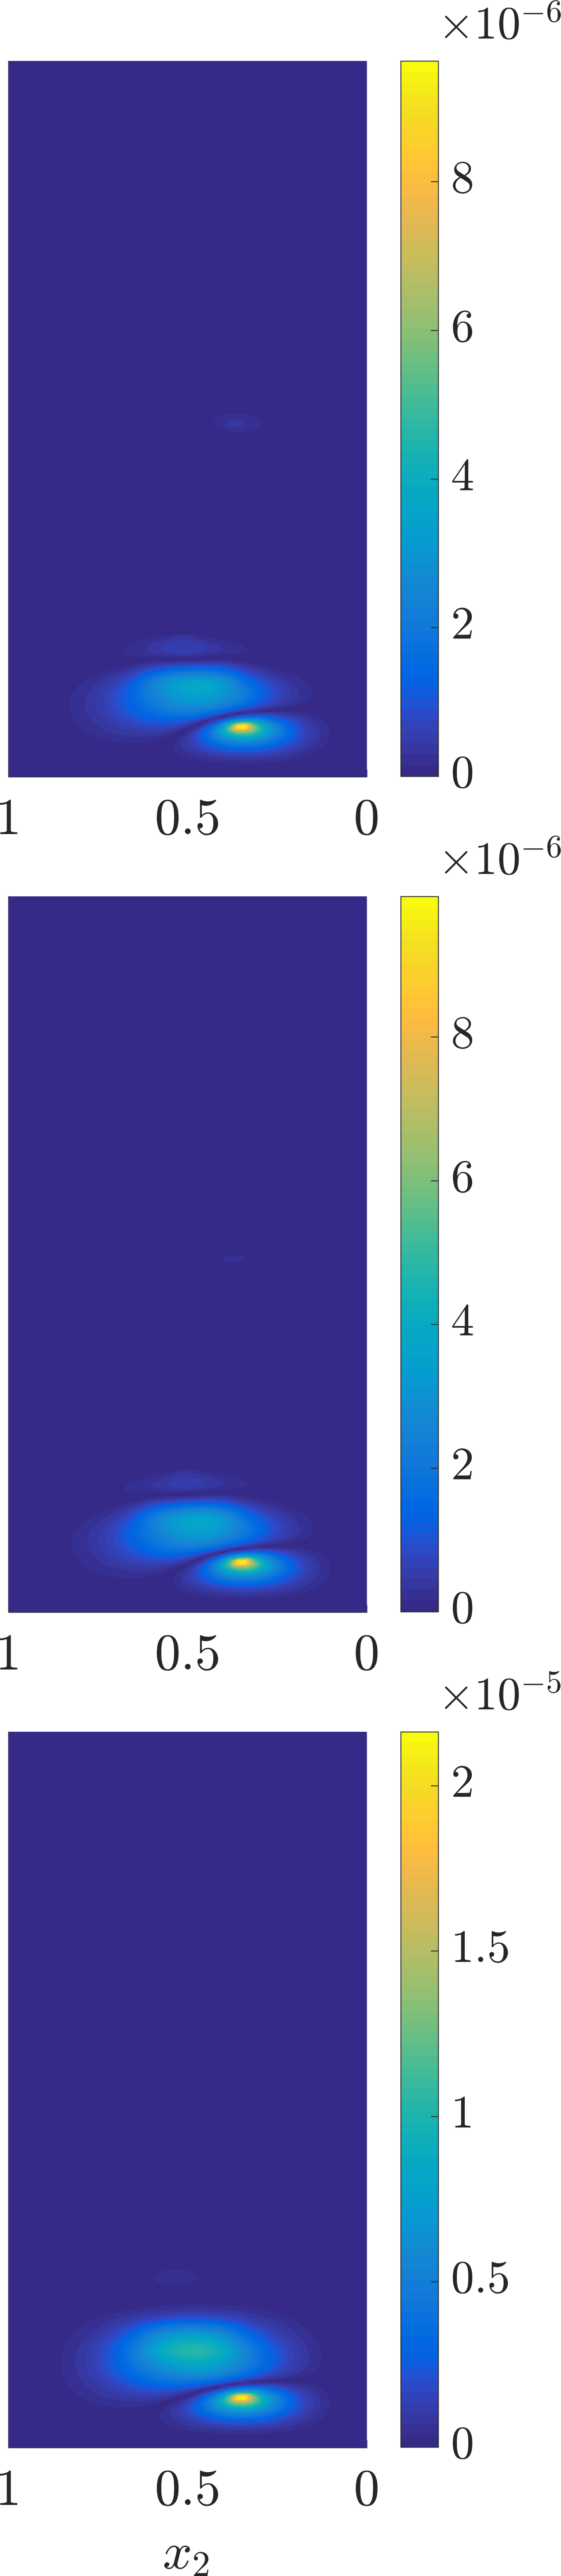
\includegraphics[width=0.23\textwidth]{vs_data/vs_data_err0.png}
%DIFDELCMD <   %DIFDELCMD < \label{subfig:obsLF2}%%%
%DIFDELCMD < }
%DIFDELCMD < \subfloat[MF$_1$ ($\sim5\%$ HF)][MF$_1$ \\($\sim5\%$ HF)]{
%DIFDELCMD <   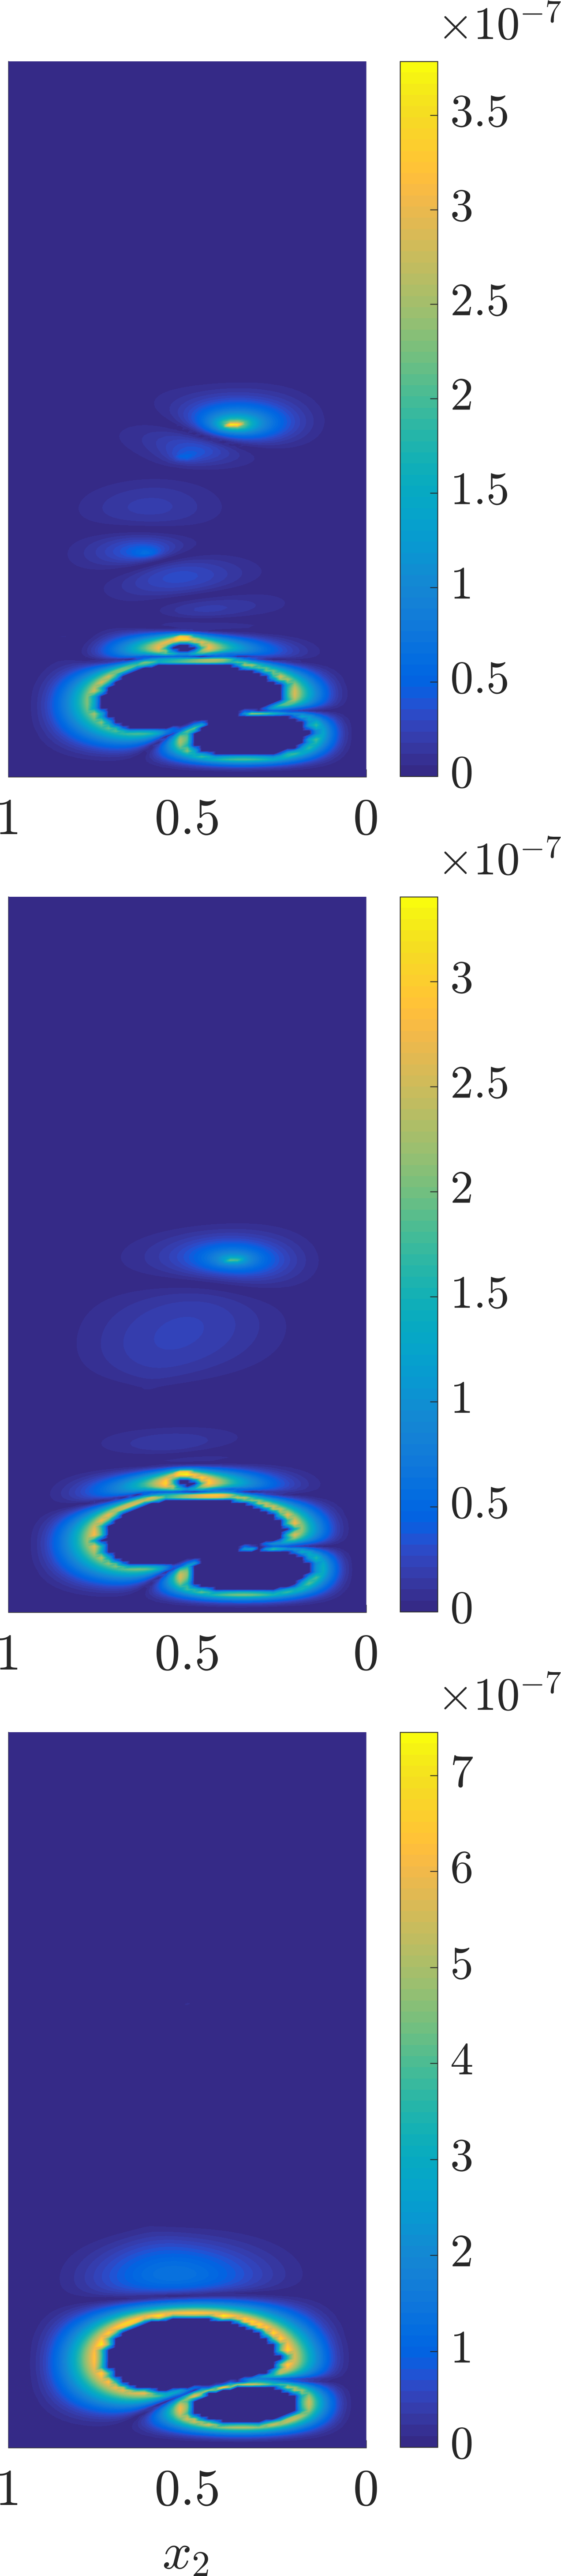
\includegraphics[width=0.23\textwidth]{vs_data/vs_data_err1.png}
%DIFDELCMD < }
%DIFDELCMD < \subfloat[MF$_2$ ($\sim10\%$ HF)][MF$_2$ \\($\sim10\%$ HF)]{
%DIFDELCMD <   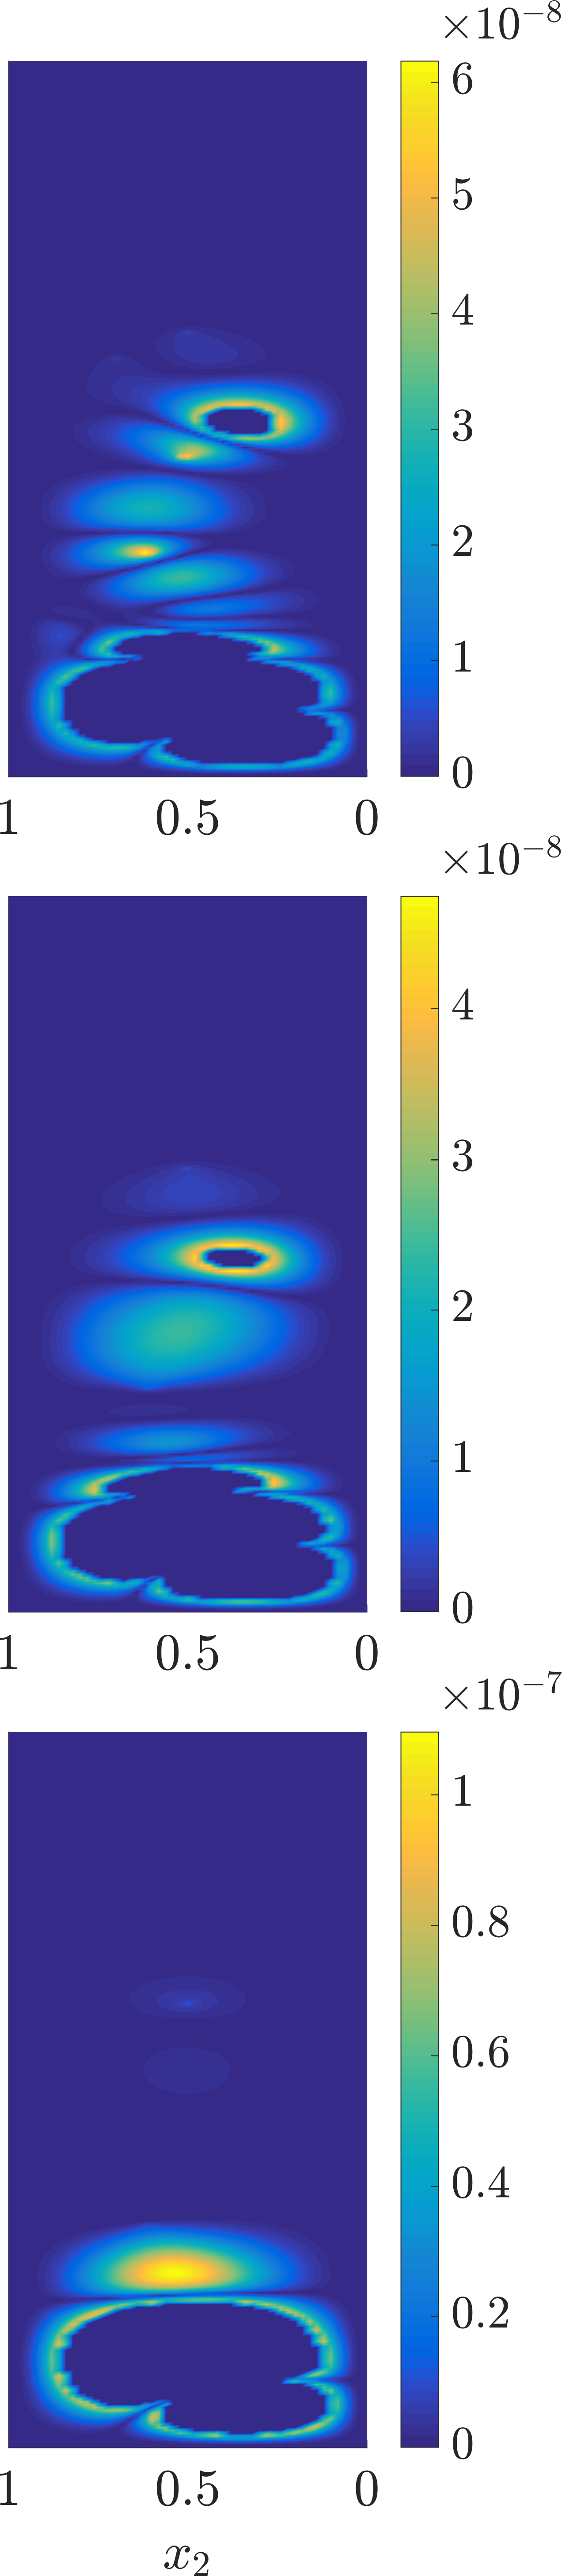
\includegraphics[width=0.23\textwidth]{vs_data/vs_data_err2.png}
%DIFDELCMD <   %DIFDELCMD < \label{subfig:obsMFlast2}%%%
%DIFDELCMD < }
%DIFDELCMD <   %%%
\DIFdelendFL \DIFaddbeginFL \captionsetup{justification=centering}
\subfloat[Locations of observations and QoI region $\Omega_I$][Locations of \\observations and \\QoI region $\Omega_I$]{
  %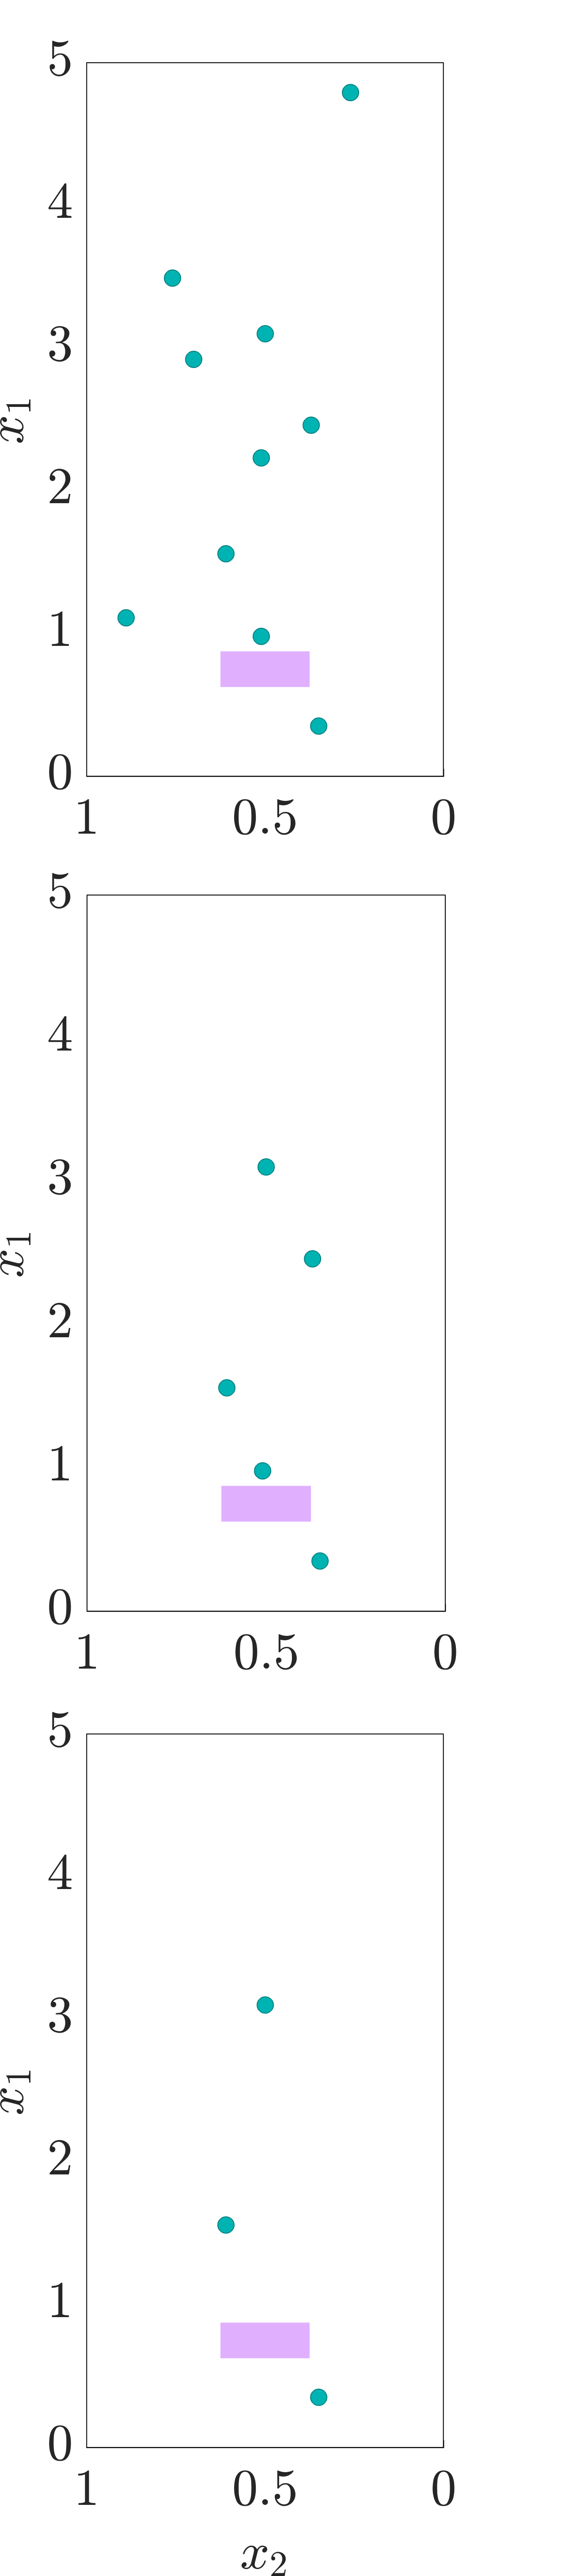
\includegraphics[width=0.23\textwidth]{vs_data/vs_data_setup.png}
  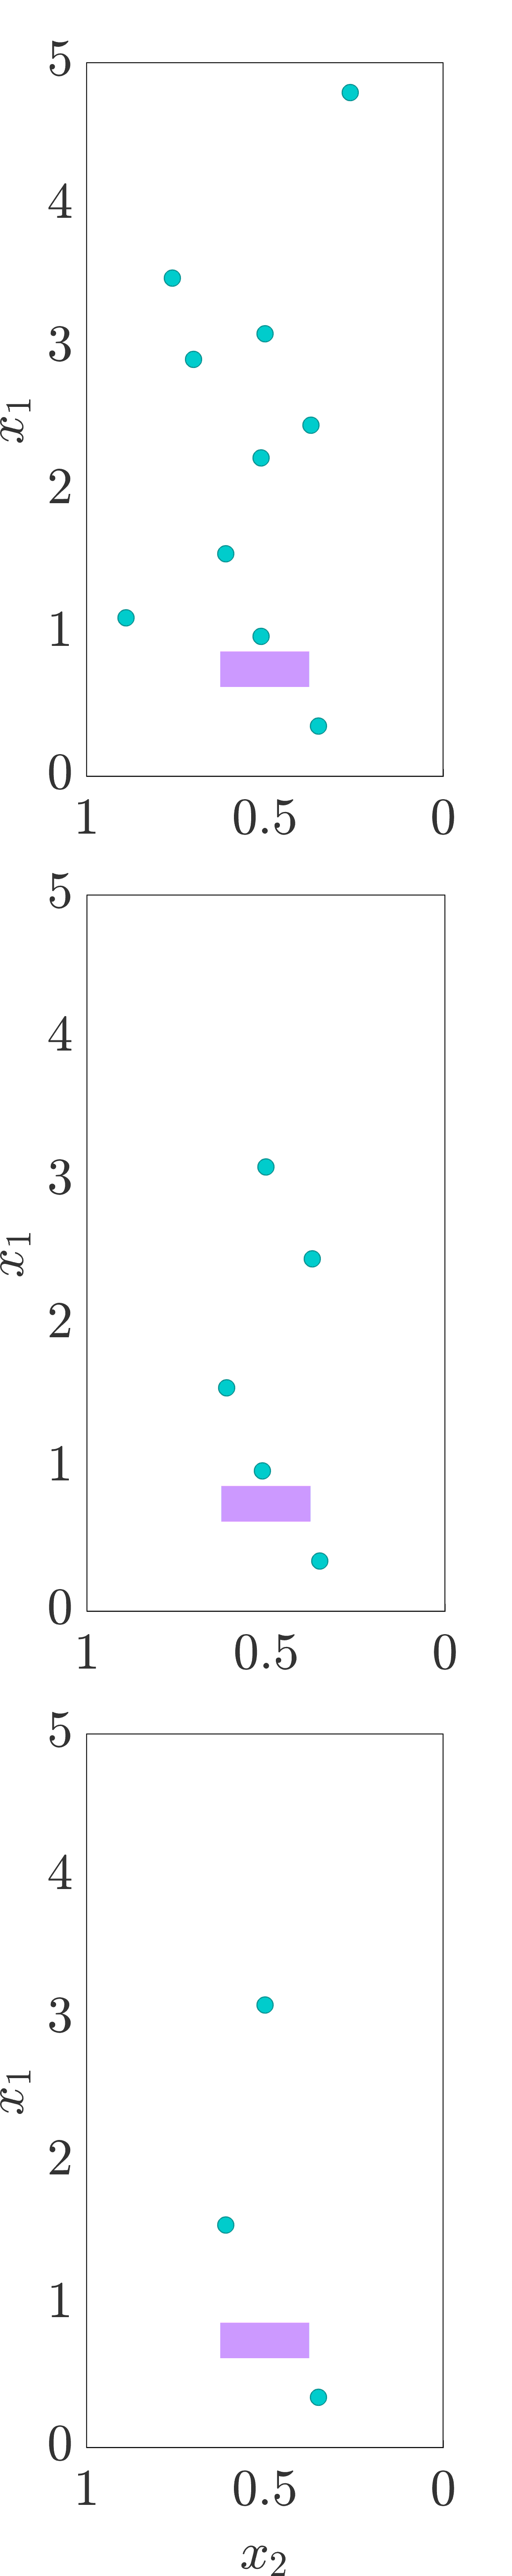
\includegraphics[width=0.21\textwidth]{vs_data/vs_data_setup_sidetrim.png}
  \label{subfig:obsSetup2}
}
\captionsetup{justification=centering}
\subfloat[MF$_0$ ($0\%$ HF)][MF$_0$ \\($0\%$ HF)]{
  %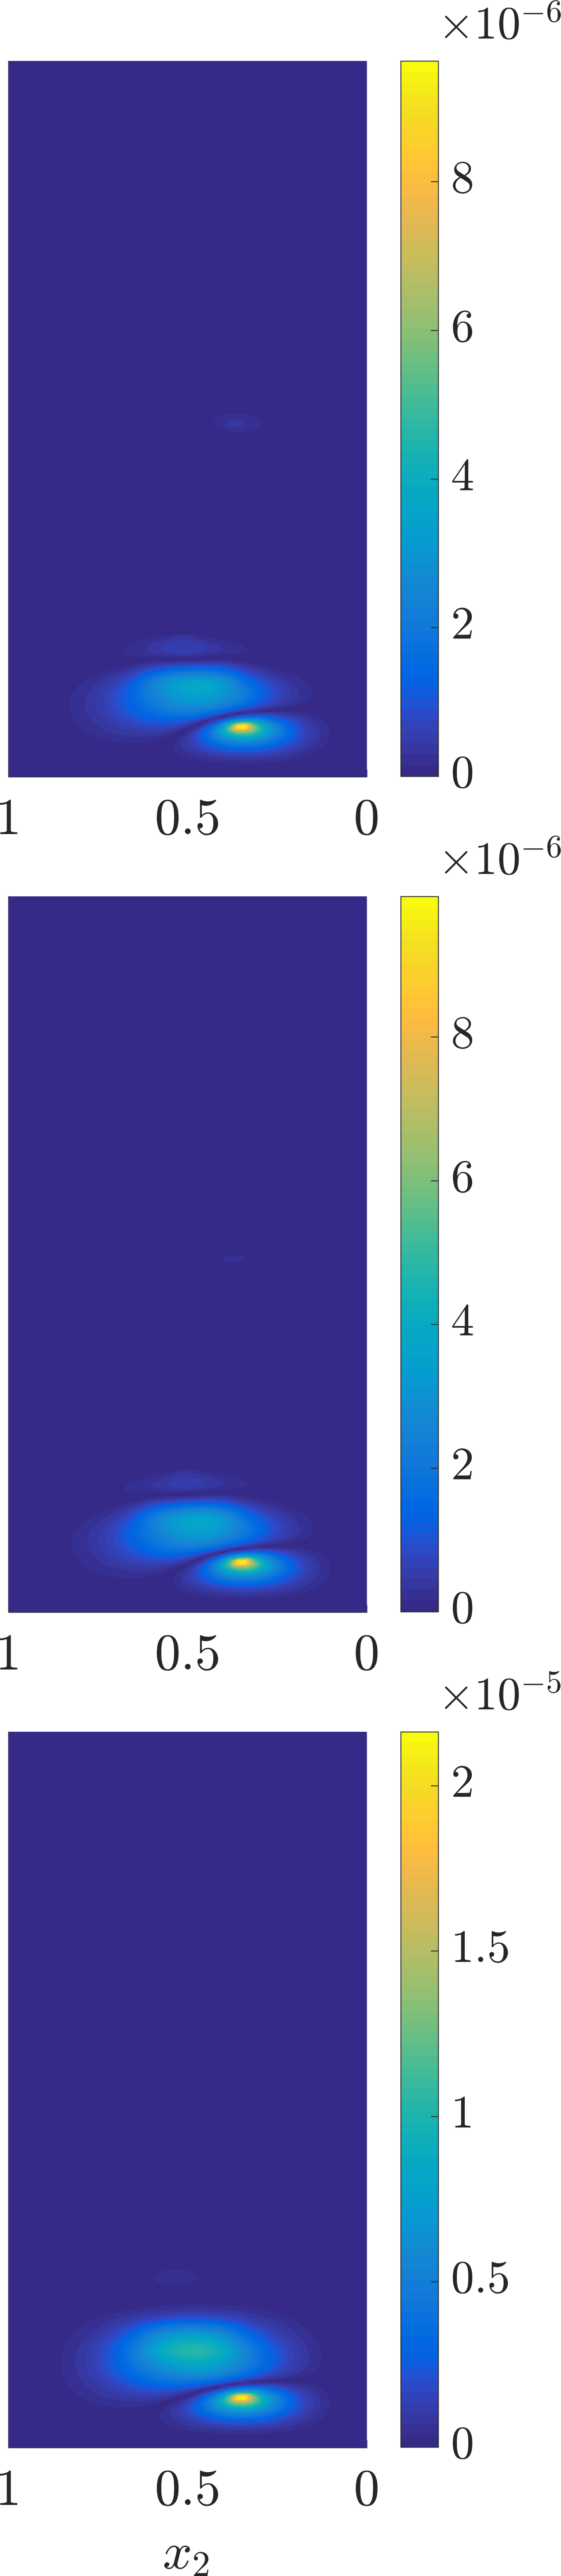
\includegraphics[width=0.23\textwidth]{vs_data/vs_data_err0.png}
  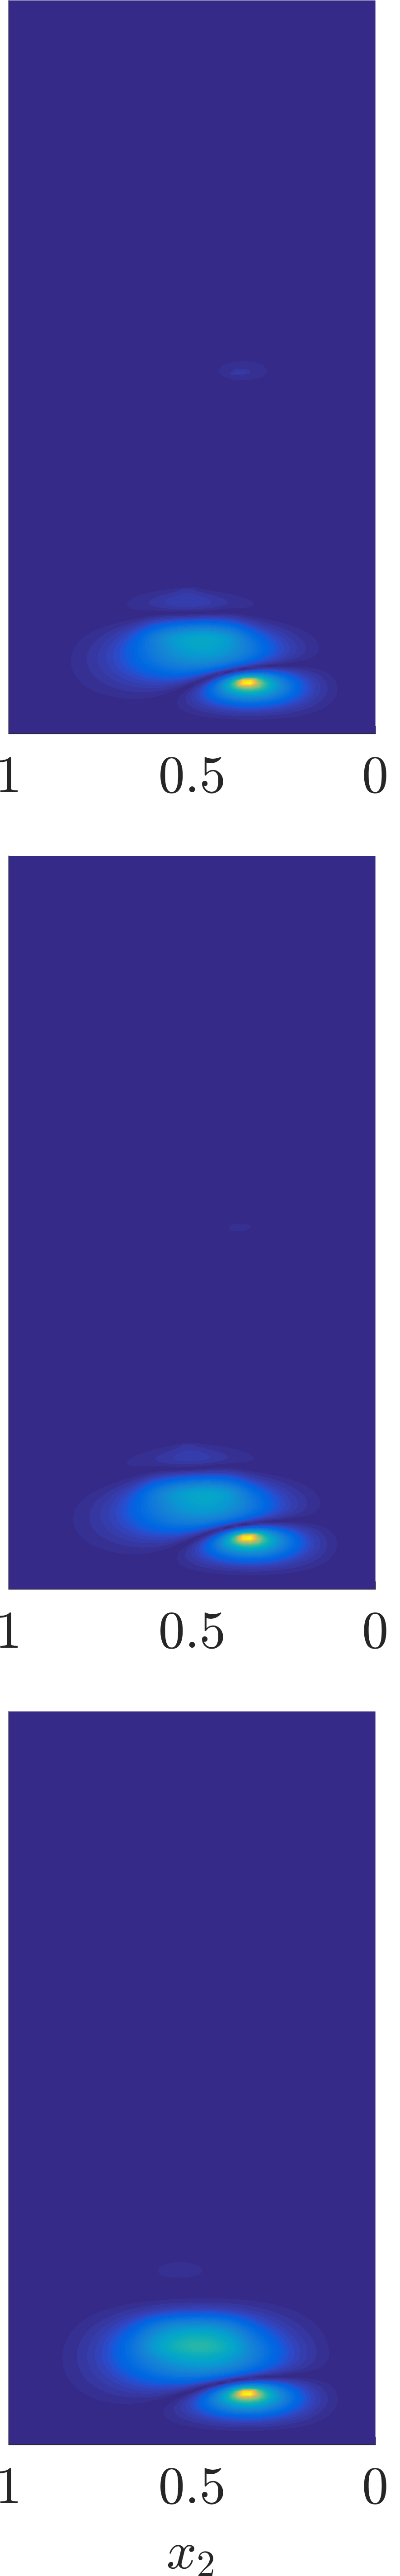
\includegraphics[width=0.16\textwidth]{vs_data/vs_data_err0_nobar.png}
  \label{subfig:obsLF2}
}
\captionsetup{justification=centering}
\subfloat[MF$_1$ ($\sim5\%$ HF)][MF$_1$ \\($\sim5\%$ HF)]{
  %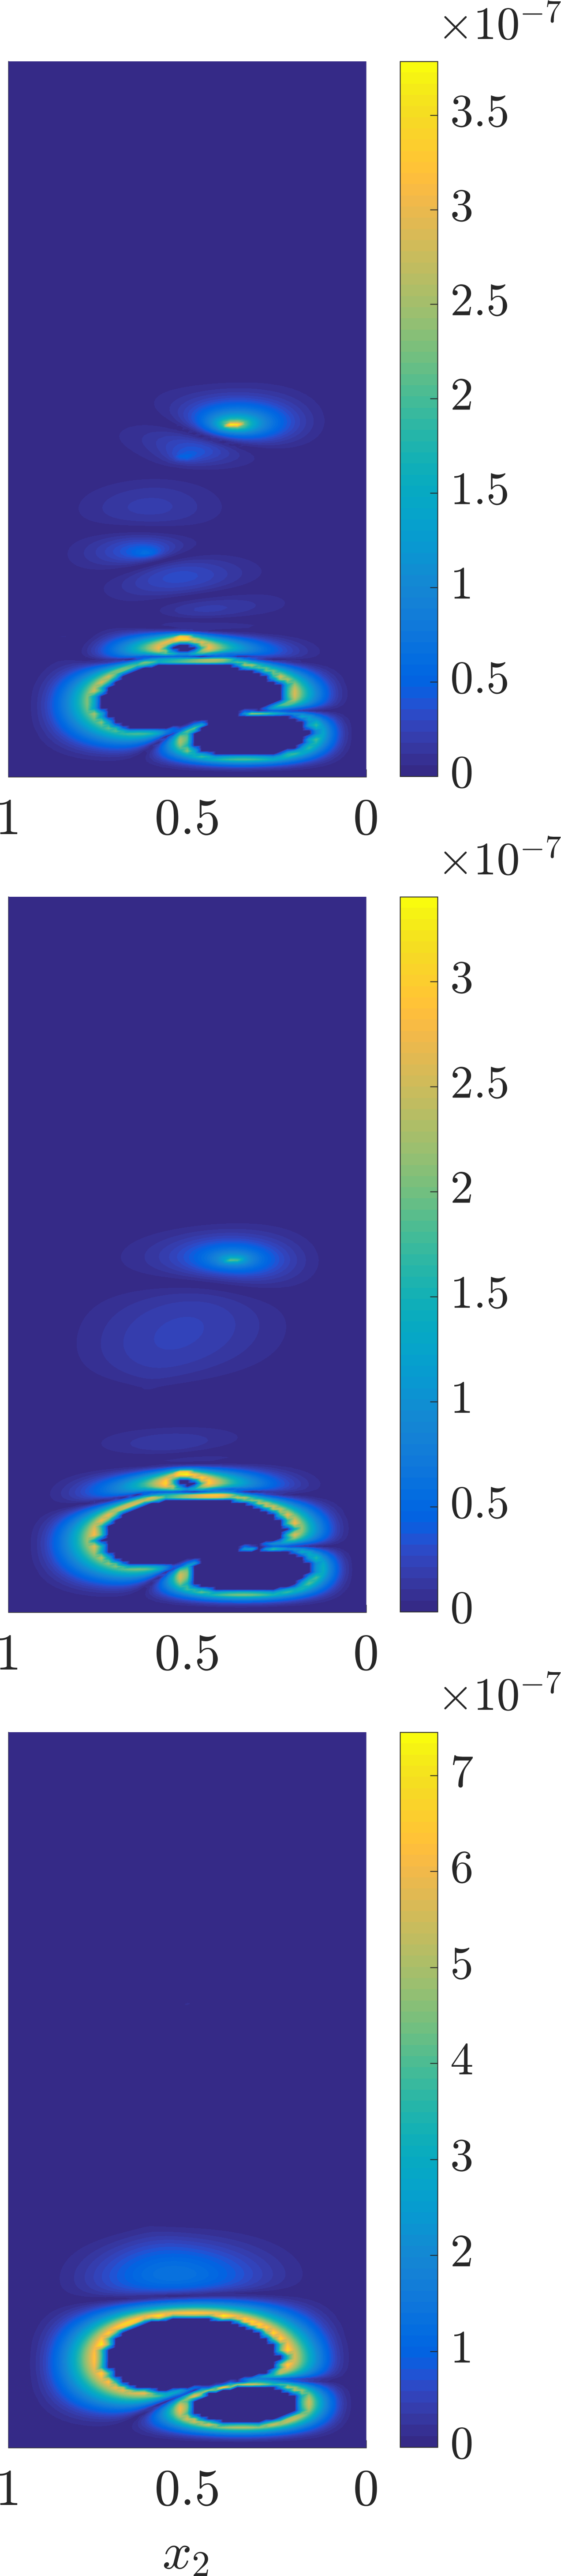
\includegraphics[width=0.23\textwidth]{vs_data/vs_data_err1.png}
  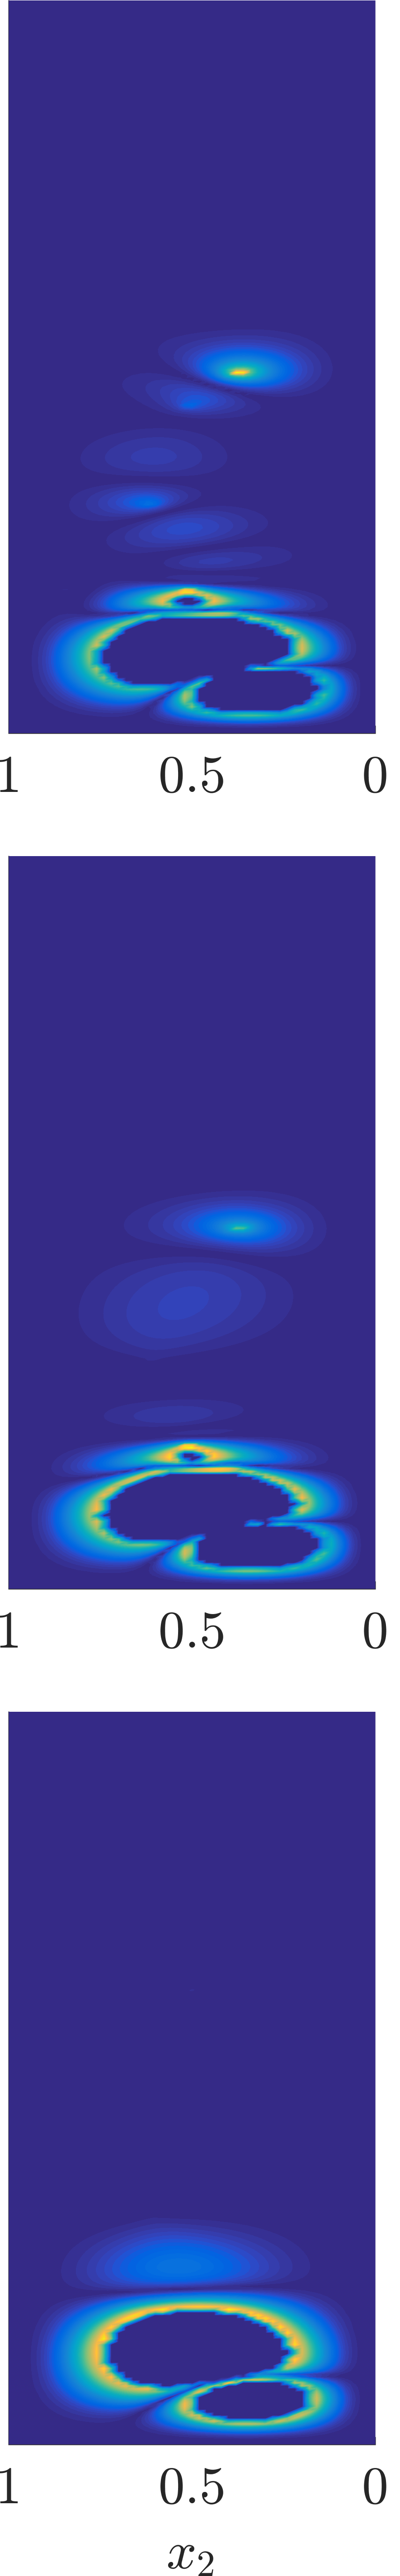
\includegraphics[width=0.16\textwidth]{vs_data/vs_data_err1_nobar.png}
}
\captionsetup{justification=centering}
\subfloat[MF$_2$ ($\sim10\%$ HF)][MF$_2$ \\($\sim10\%$ HF)]{
  %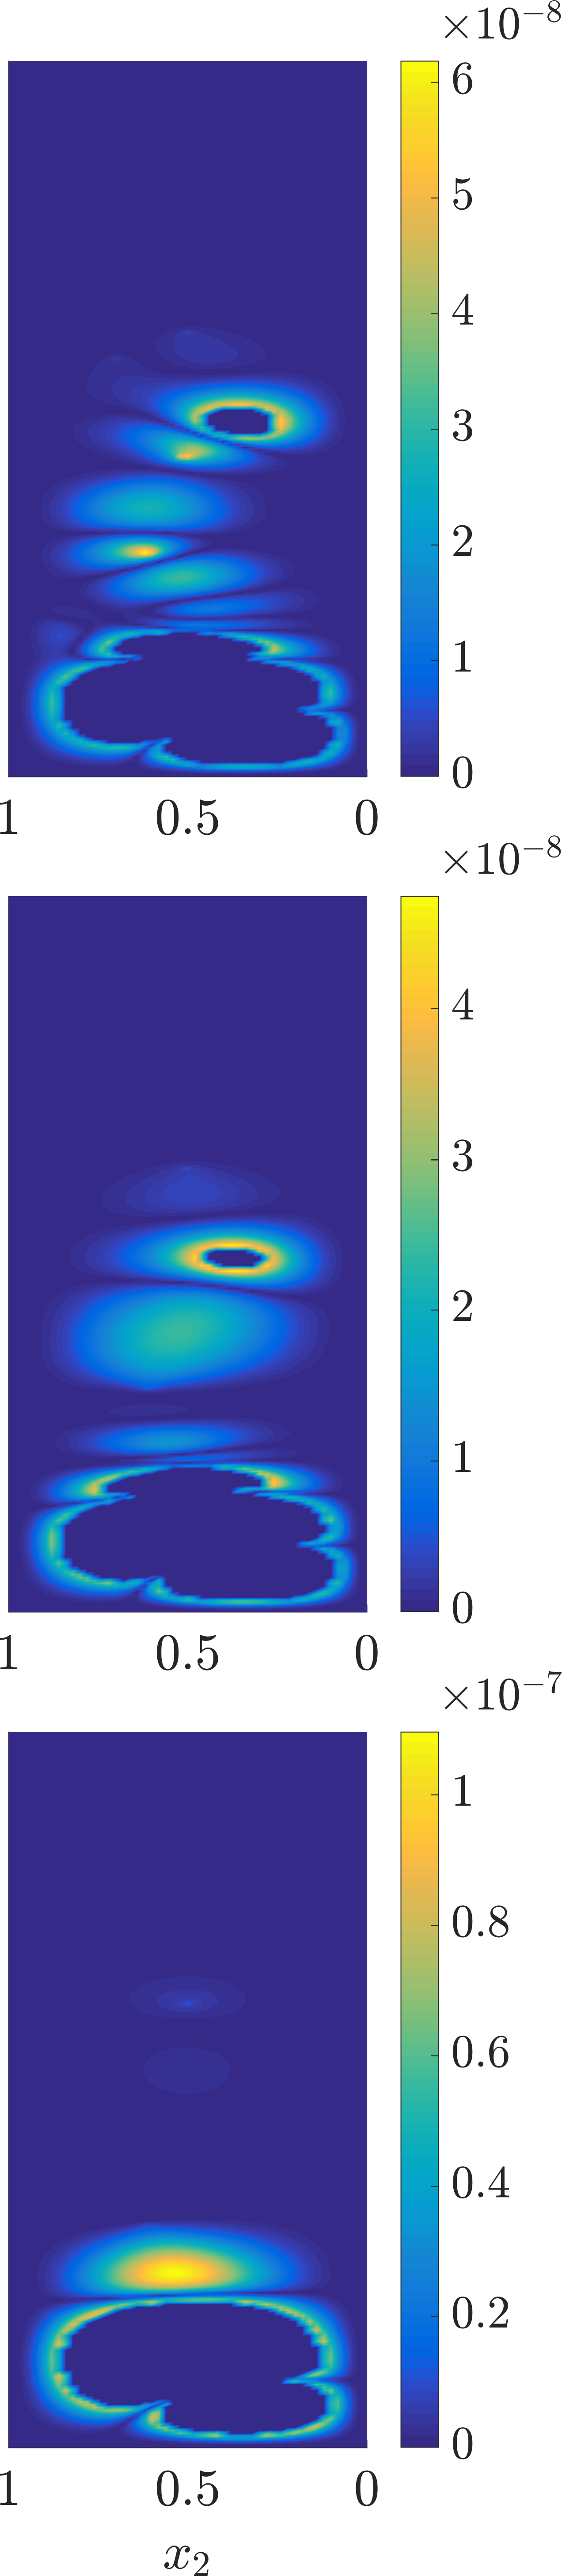
\includegraphics[width=0.23\textwidth]{vs_data/vs_data_err2.png}
  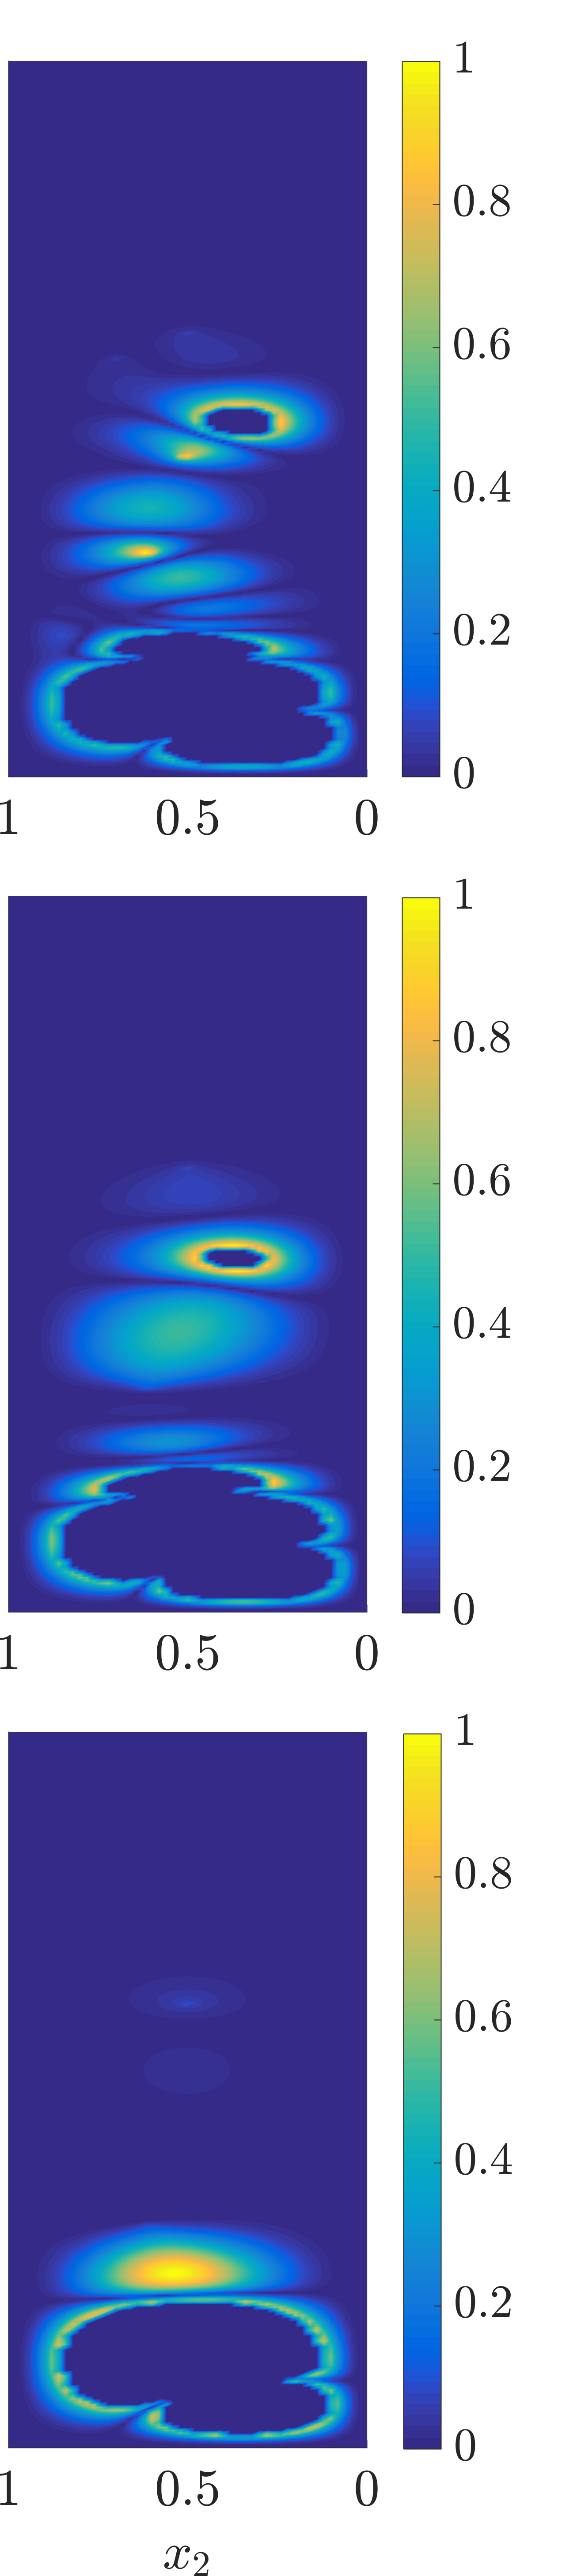
\includegraphics[width=0.23\textwidth]{vs_data/vs_data_err2_barnorm.png}
  \label{subfig:obsMFlast2}
}
  \DIFaddendFL \caption{Effects of increasing the number of observations. Column \protect\subref{subfig:obsSetup2}: configuration of observations (teal points) and QoI region (purple box). Columns \protect\subref{subfig:obsLF2}--\protect\subref{subfig:obsMFlast2}): the \DIFaddbeginFL \DIFaddFL{relative }\DIFaddendFL error estimate decompositions for different mixed-fidelity models\DIFaddbeginFL \DIFaddFL{, relative to the largest localized error contribution; note the locations of regions of relatively large error compared to the observation locations and QoI region}\DIFaddendFL .}
  \label{fig:dataStudy}
\end{figure}

%------------------------------------------------------------------------------------------------------------------------%
\subsection{Variable Parameterization: Constant vs.\ Field Parameters} \label{sec:constvfield}
%------------------------------------------------------------------------------------------------------------------------%

In this subsection, we consider two models which differ in the space to which the parameter belongs, with the low-fidelity model having fewer degrees of freedom. 

%------------------------------------------------------------%
\subsubsection{Problem Setup}
%------------------------------------------------------------%

We consider the same high-fidelity model as in \cref{sec:cdvcdr}:
\begin{equation}
k_d\nabla^2 u - \vec{V}\cdot\nabla u + k_ru^2= f(q),\quad q\in U,
\end{equation}
with the same diffusion coefficient $k_d = 0.1$  and reaction coefficient $k_r = -42$. The low-fidelity model
\begin{equation}
k_d\nabla^2 u - \vec{V}\cdot\nabla u + k_ru^2= f(q),\quad q\in\R
\end{equation}
differs from the high-fidelity model only in that the parameter $q$ is a constant instead of a field. The intermediate mixed-fidelity models thus have parameter fields that are constant over the subregions of the domain where the low-fidelity model is used. For ease of implementation, we require that the resulting parameter field remain continuous at the interface between the low-fidelity and high-fidelity subdomains, although this constraint is not necessary for the theory to hold. The domain, mesh, boundary conditions, and velocity field, as well as the observations, unknown parameters to be inferred, and QoI, remain the same as described in \cref{sec:cdvcdr}. As the inverse problem is ill-posed, except \DIFdelbegin \DIFdel{for perhaps %DIF <  KW: is it or not?
in the case where the }\DIFdelend \DIFaddbegin \DIFadd{when the }\DIFaddend low-fidelity model is used throughout the domain, regularization is \DIFdelbegin \DIFdel{added; %DIF <  KW: added to what?
 }\DIFdelend \DIFaddbegin \DIFadd{used; }\DIFaddend the Tikhonov regularization term \DIFdelbegin \DIFdel{is $\frac{\beta}{2}\int_\Omega \|\nabla f(q)\|_2^2+f(q)^2\:\textrm{d}A$}\DIFdelend \DIFaddbegin \DIFadd{in }\cref{eq:invOpt_obj} \DIFadd{is $R(q)=\frac{\beta}{2}\int_\Omega \|\nabla f(q)\|_2^2+f(q)^2\:\textrm{d}A$}\DIFaddend , where $\beta=10^{-3}$ is a regularization coefficient. 
%DIF <  KW: refer to the actual equation you are adding regularization to, or re-state the objective.

%DIF <  KW: I'm commenting out this next statement, unless you strongly disagree.
%DIF < Although using such a pair of models has similarities to the problem of adaptive mesh refinement, we note that in this example only the parameter field changes in its level of refinement, not the state. Should the two models differ in the resolution of the state variables instead of the parameters, it is more efficient to use the approach discussed in \cite{BecVex05}.
\DIFdelbegin %DIFDELCMD < 

%DIFDELCMD < %%%
\DIFdelend %------------------------------------------------------------%
\subsubsection{Adaptive Model Refinement Results}
%------------------------------------------------------------%

As with the previous examples in \cref{sec:cdvcdr}, the decomposition of the error estimate is used to select additional regions of the domain in which to use the high-fidelity model. The number of degrees of freedom in the inverse problem increases with the proportion of the domain in which the high-fidelity model is used. With each iteration, an additional $10\%$ of the elements are marked for refinement. This is repeated until the estimated absolute relative error in the QoI is less than $1\%$.

\Cref{fig:svfRef} shows the local error contributions, as well as the subdomains where the low- and high-fidelity models are used, for the first two and last mixed-fidelity model thus generated. 
\DIFdelbegin \DIFdel{Each linear Lagrange basis function's contribution is plotted at its nonzero node. %DIF <  KW: what does this sentence mean and is it really necessary?
}\DIFdelend %
\begin{figure}[htbp]
\centering
\subfloat[MF$_0$ ($0\%$ HF)]{
	\includegraphics[width=0.46\textwidth]{svf/cd_cdr_LF_divvy.png}
  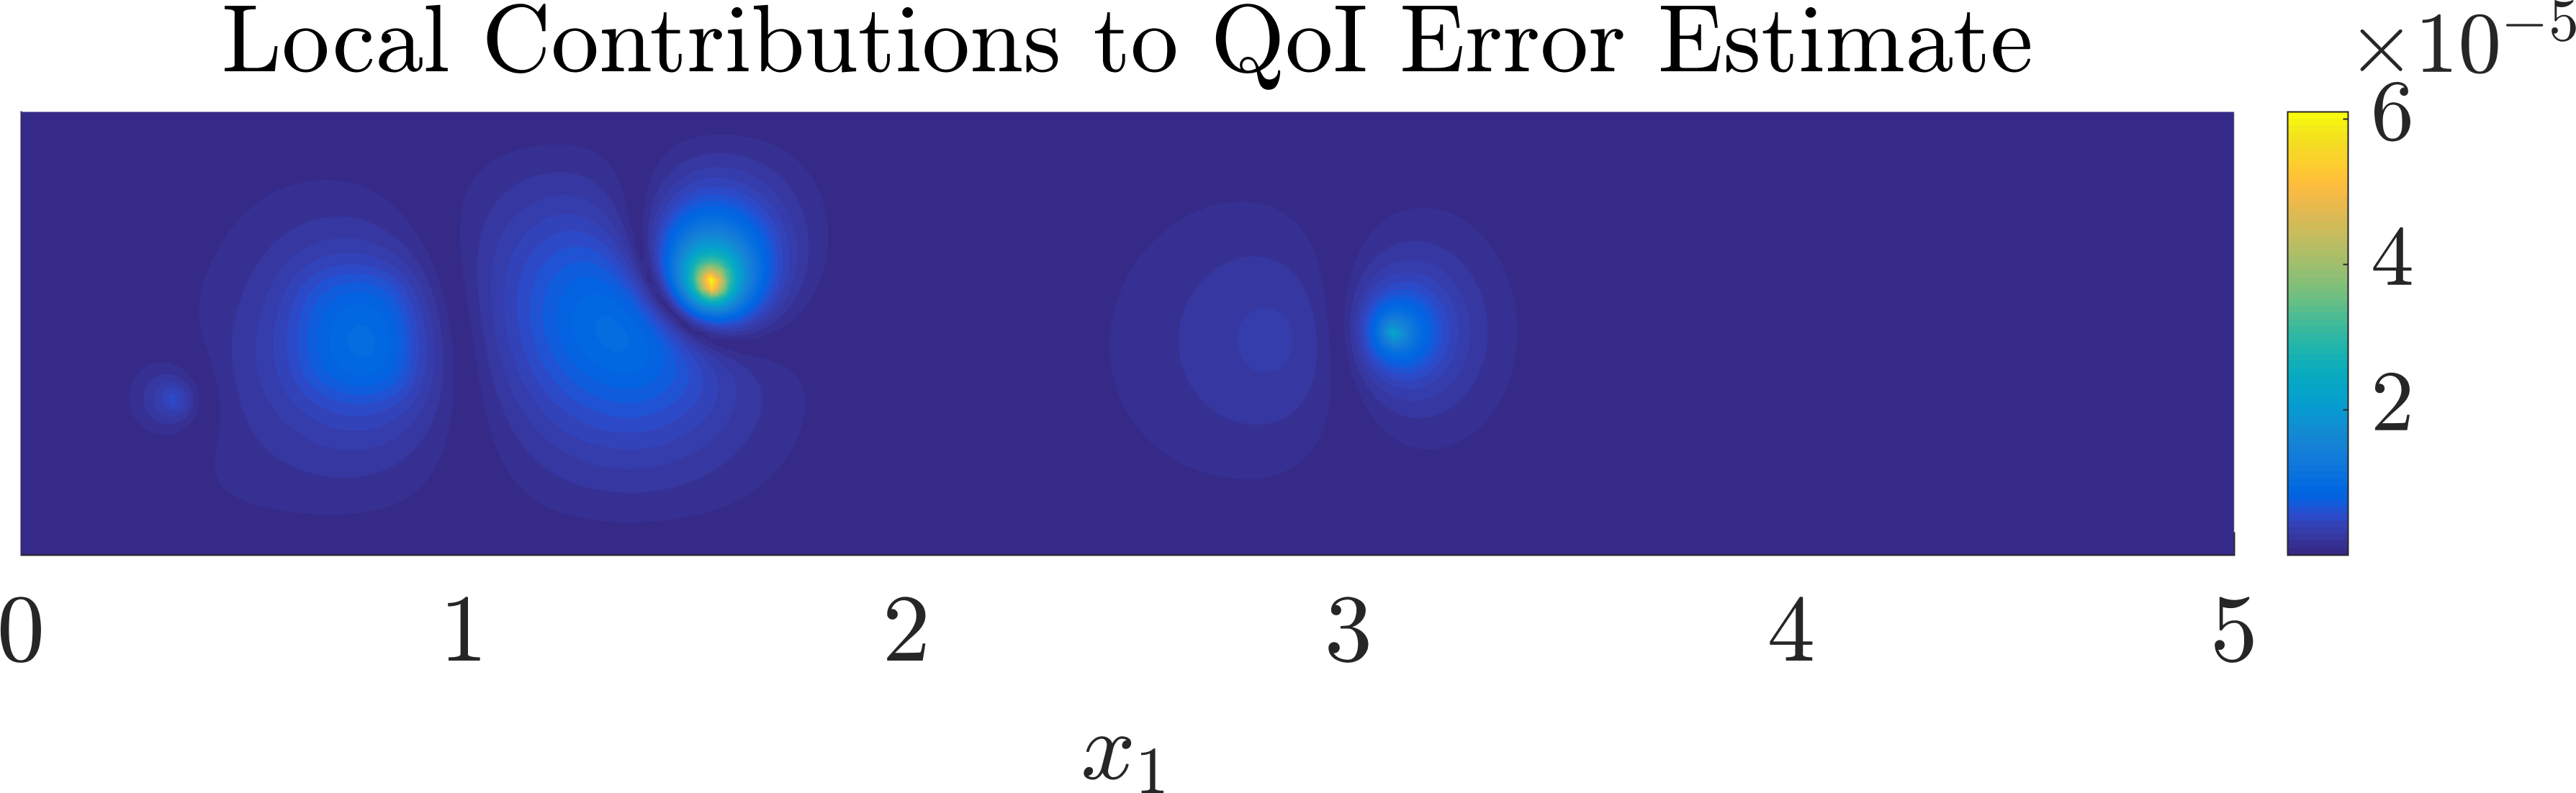
\includegraphics[width=0.49\textwidth]{svf/err_breakdown_LF.png}
} \\
\subfloat[MF$_1$ ($10\%$ HF)]{
	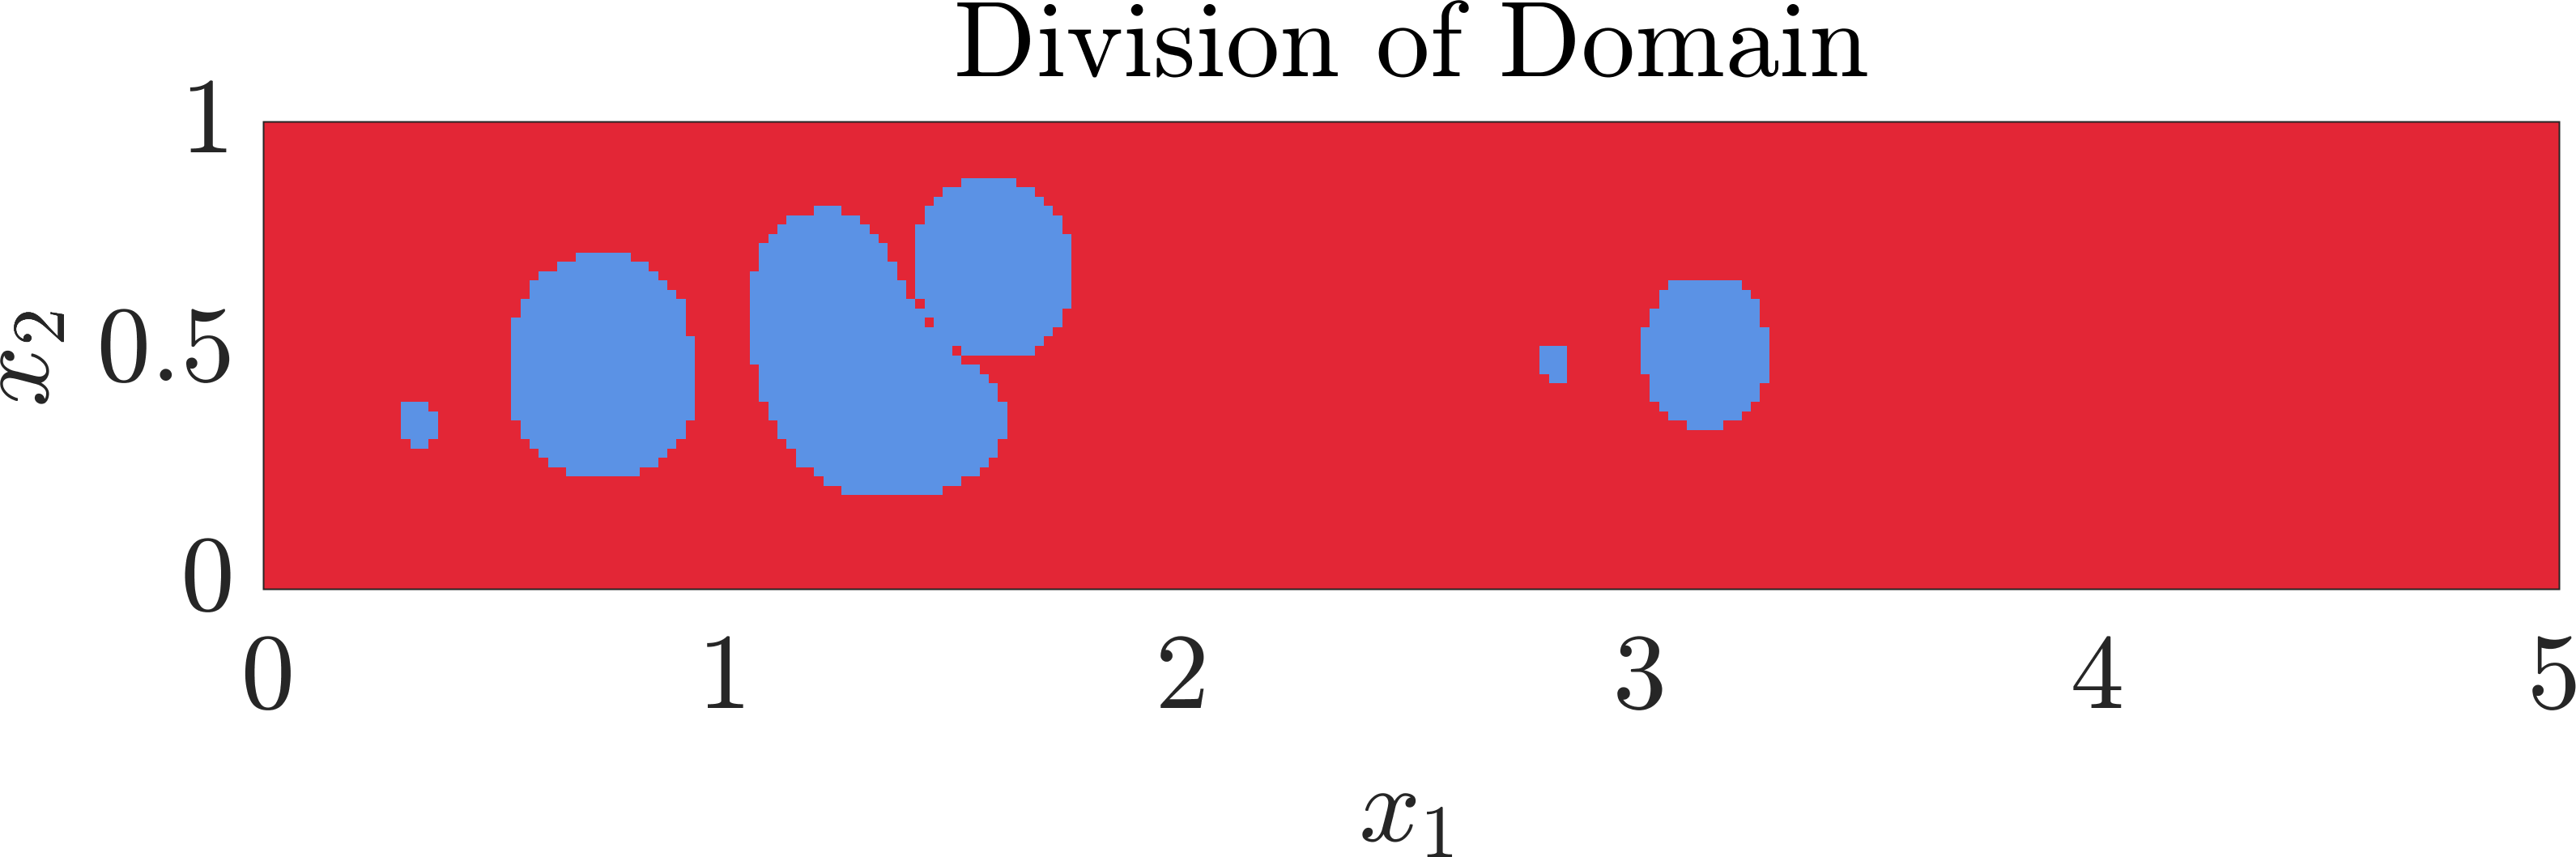
\includegraphics[width=0.46\textwidth]{svf/cd_cdr_MF01_divvy.png}
  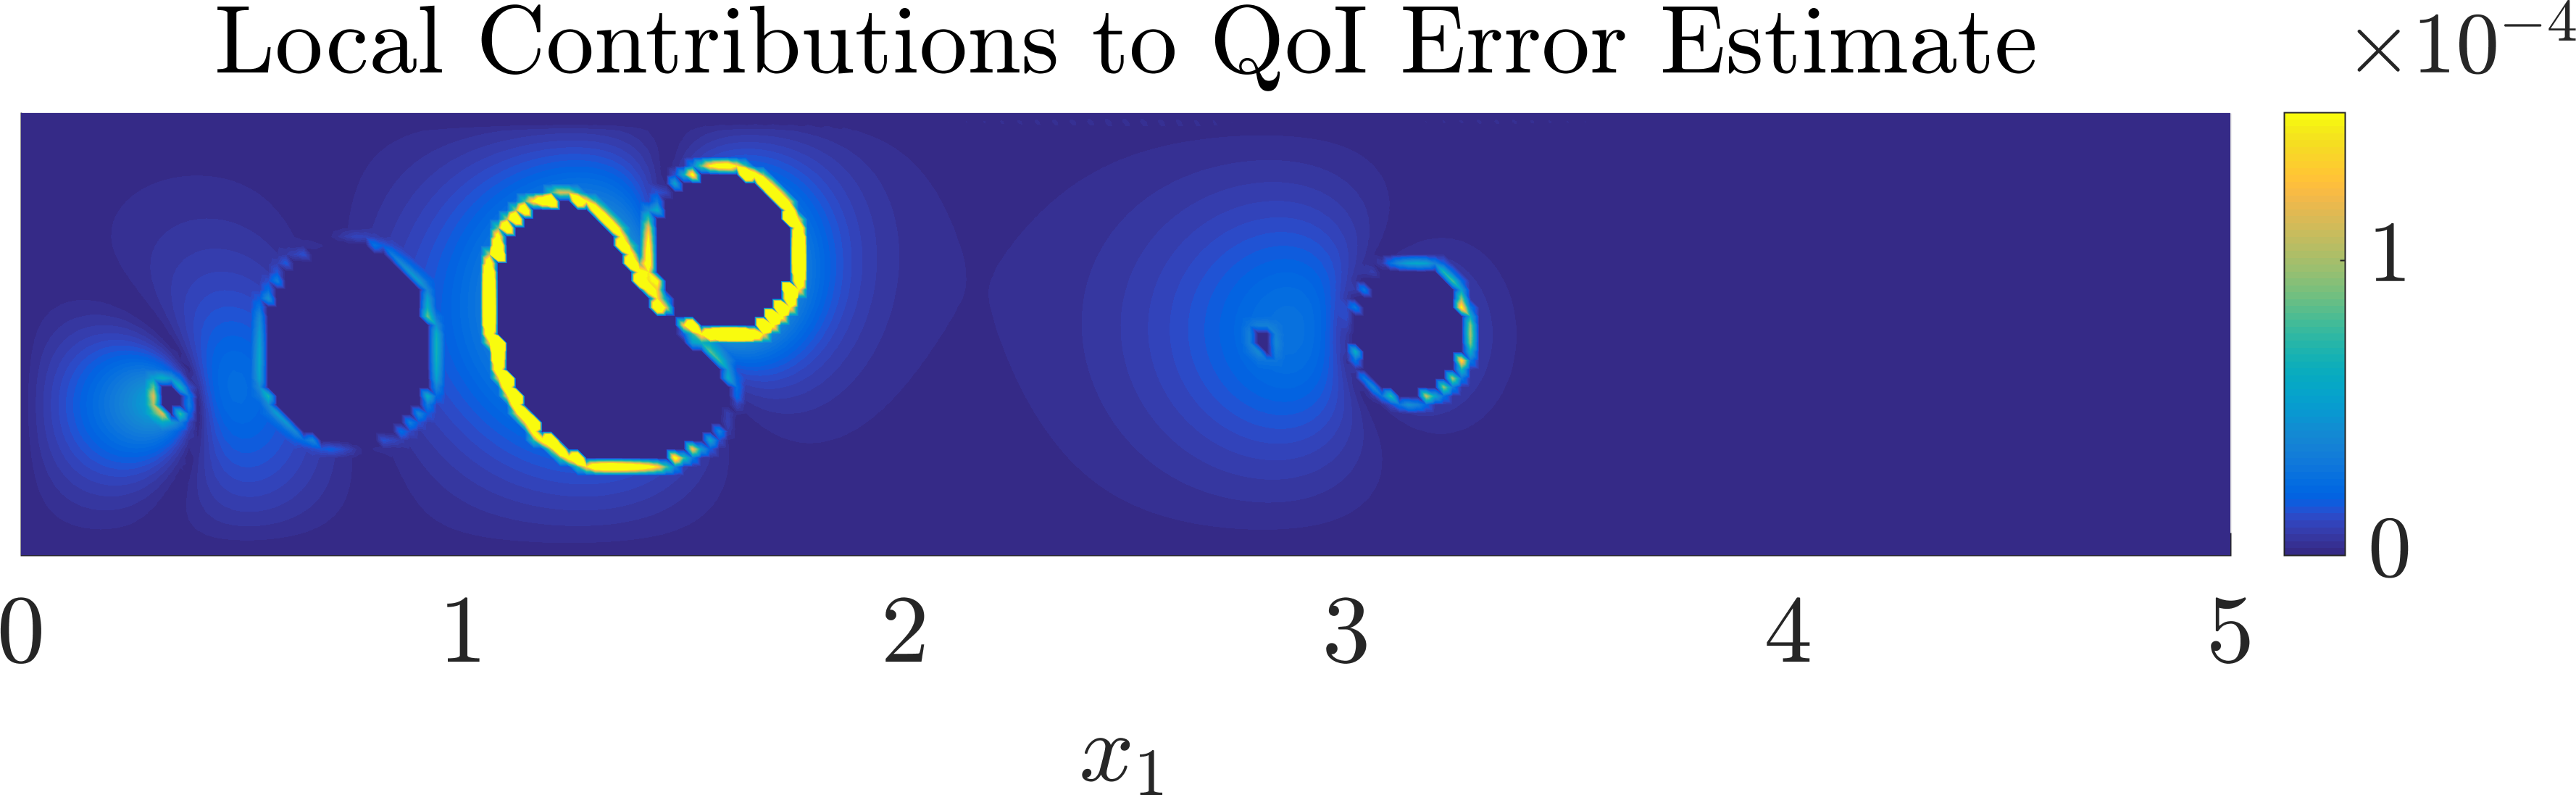
\includegraphics[width=0.49\textwidth]{svf/err_breakdown_MF01.png}
} \\
\subfloat[MF$_2$ ($20\%$ HF)]{
  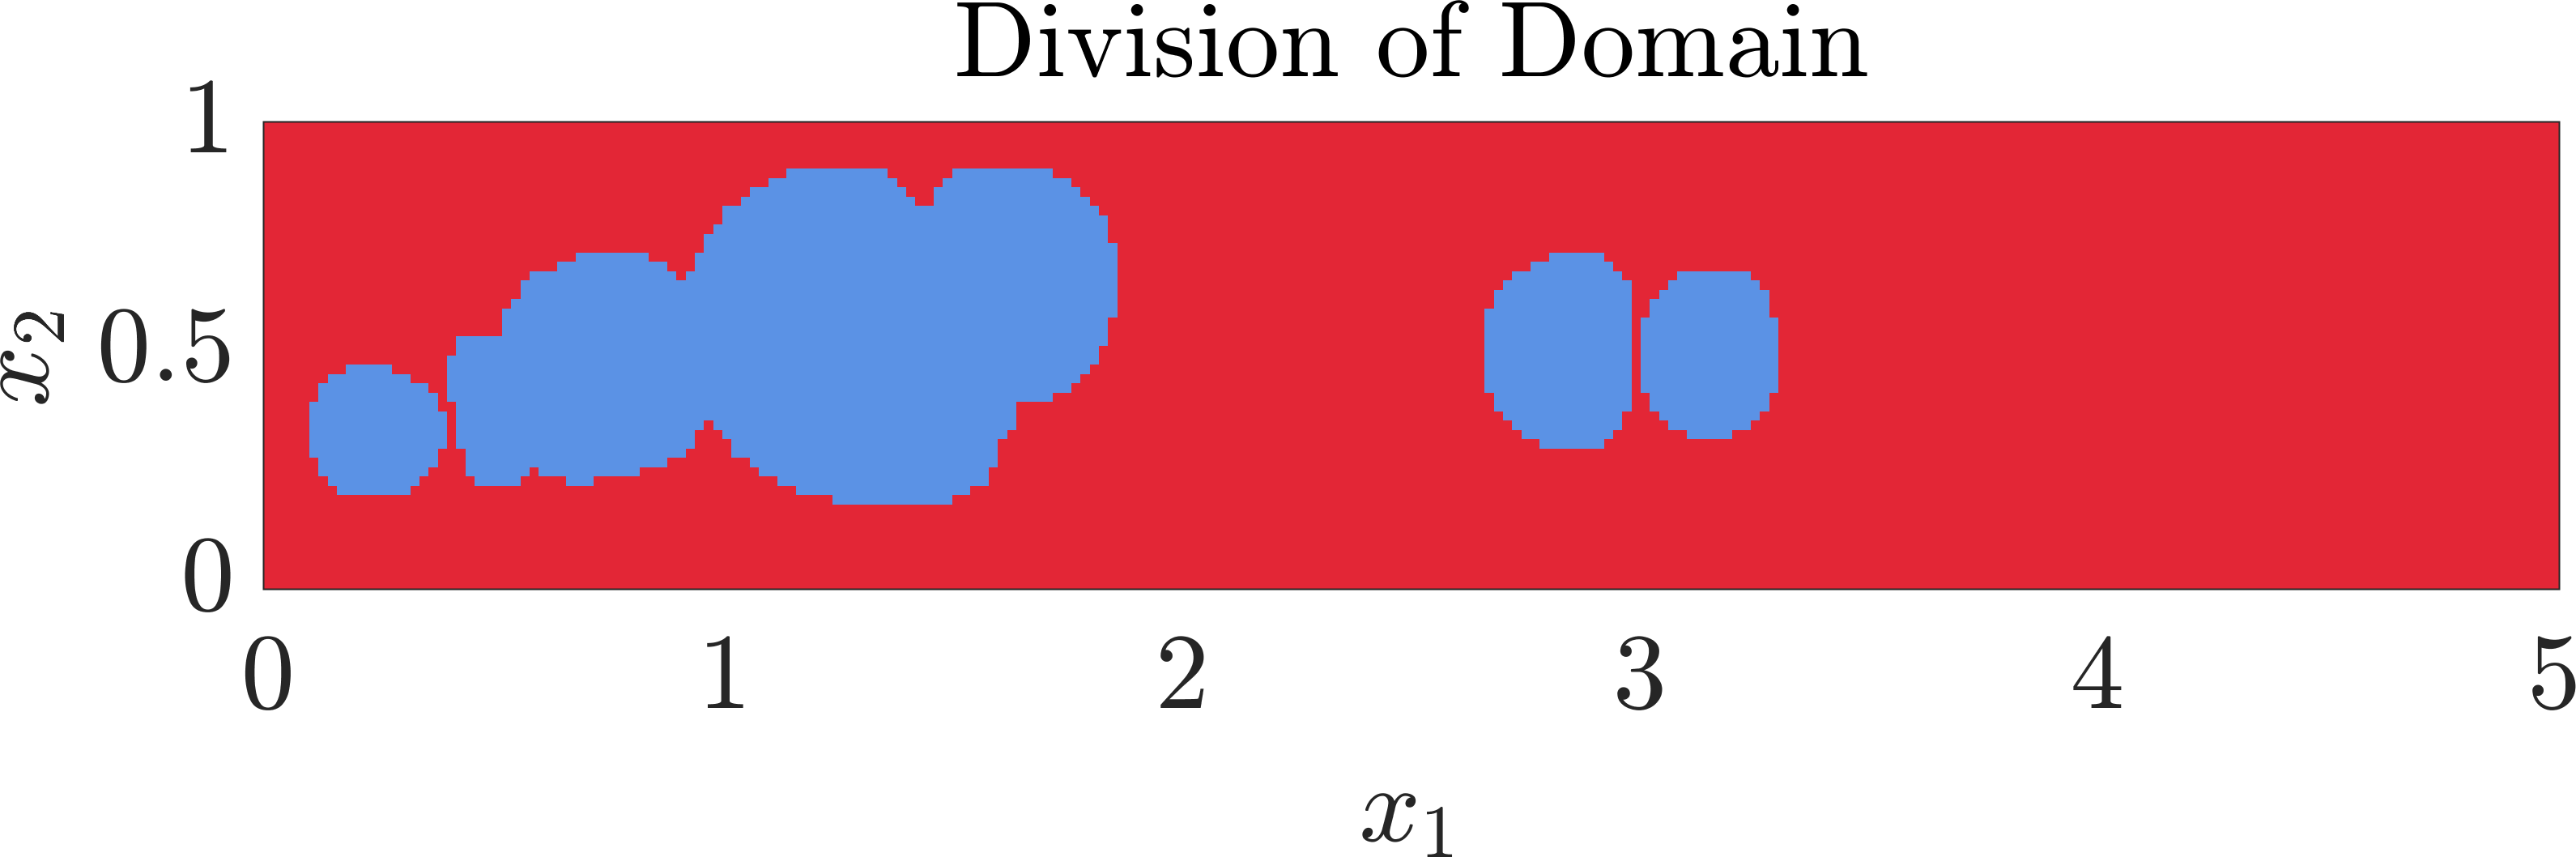
\includegraphics[width=0.46\textwidth]{svf/cd_cdr_MF02_divvy.png}
  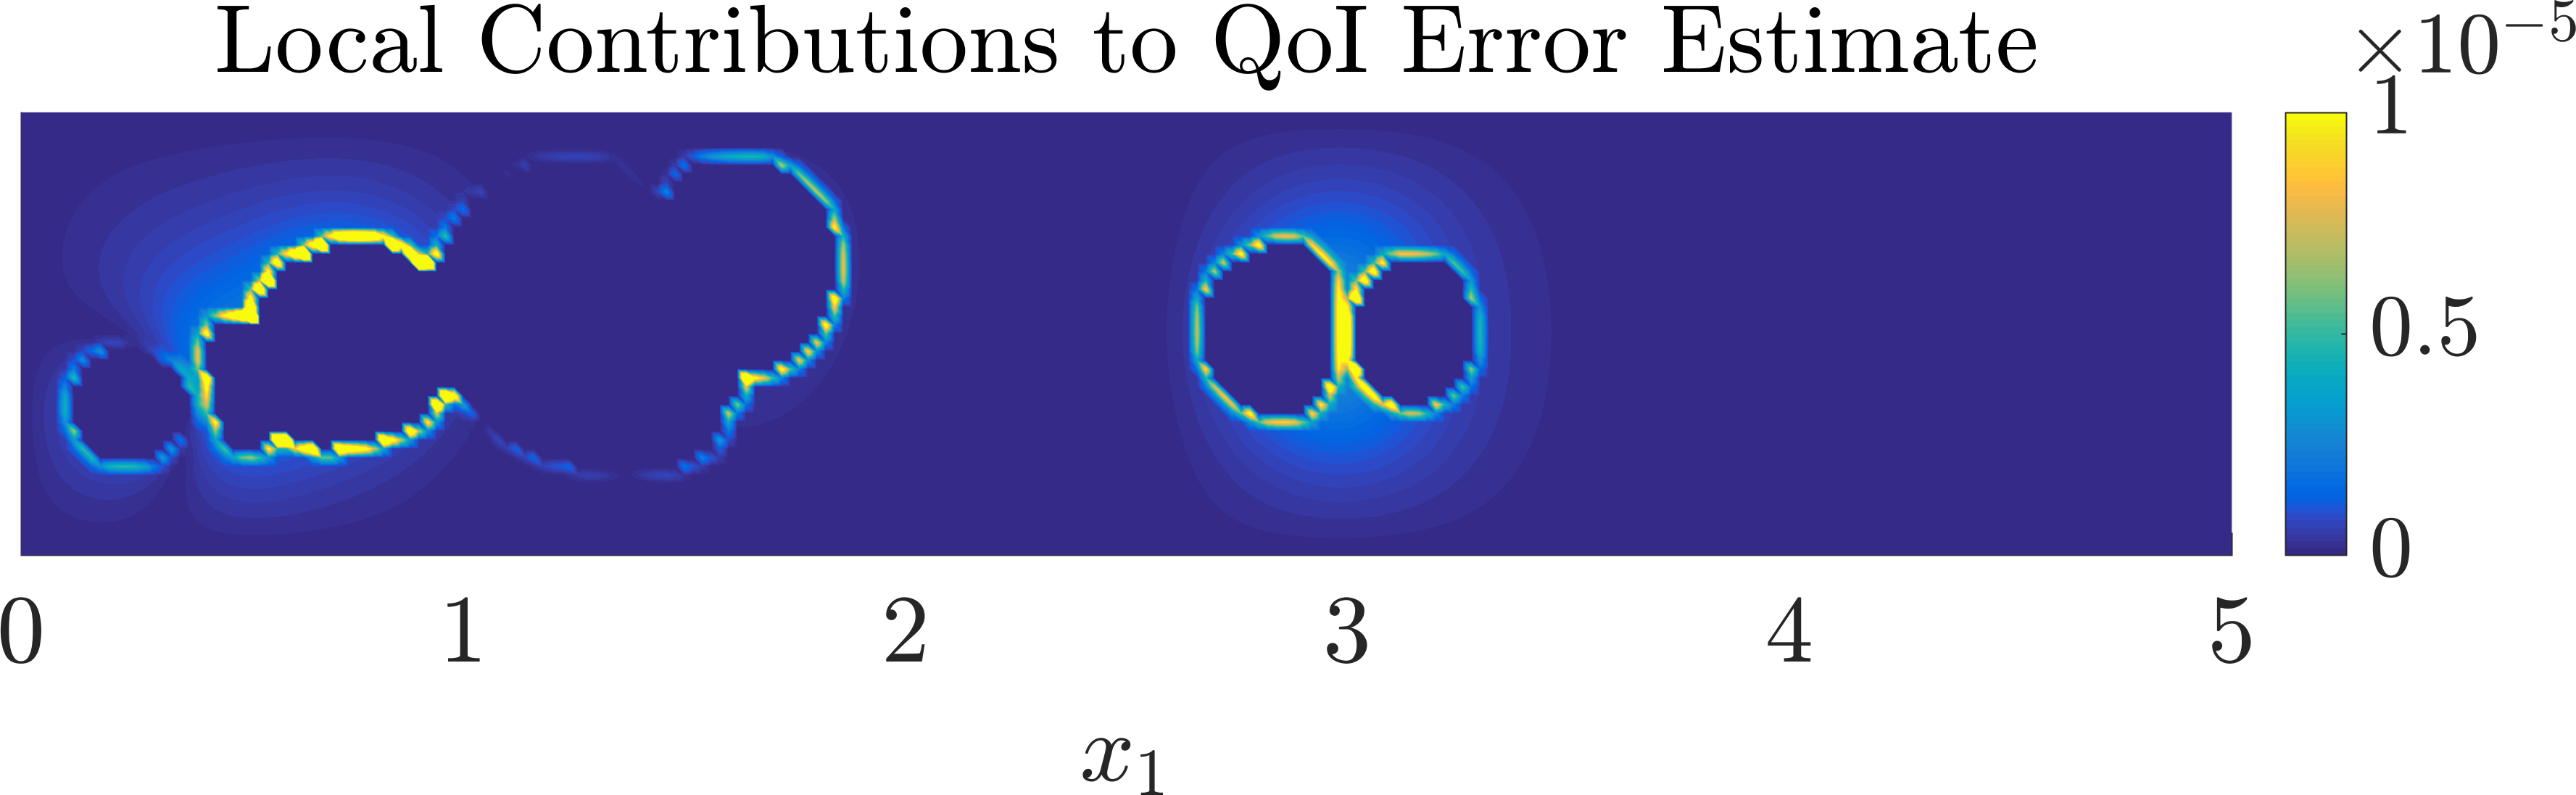
\includegraphics[width=0.49\textwidth]{svf/err_breakdown_MF02.png}
} \\
%\begin{subfigure}[b]{\textwidth}
%	\centering
%	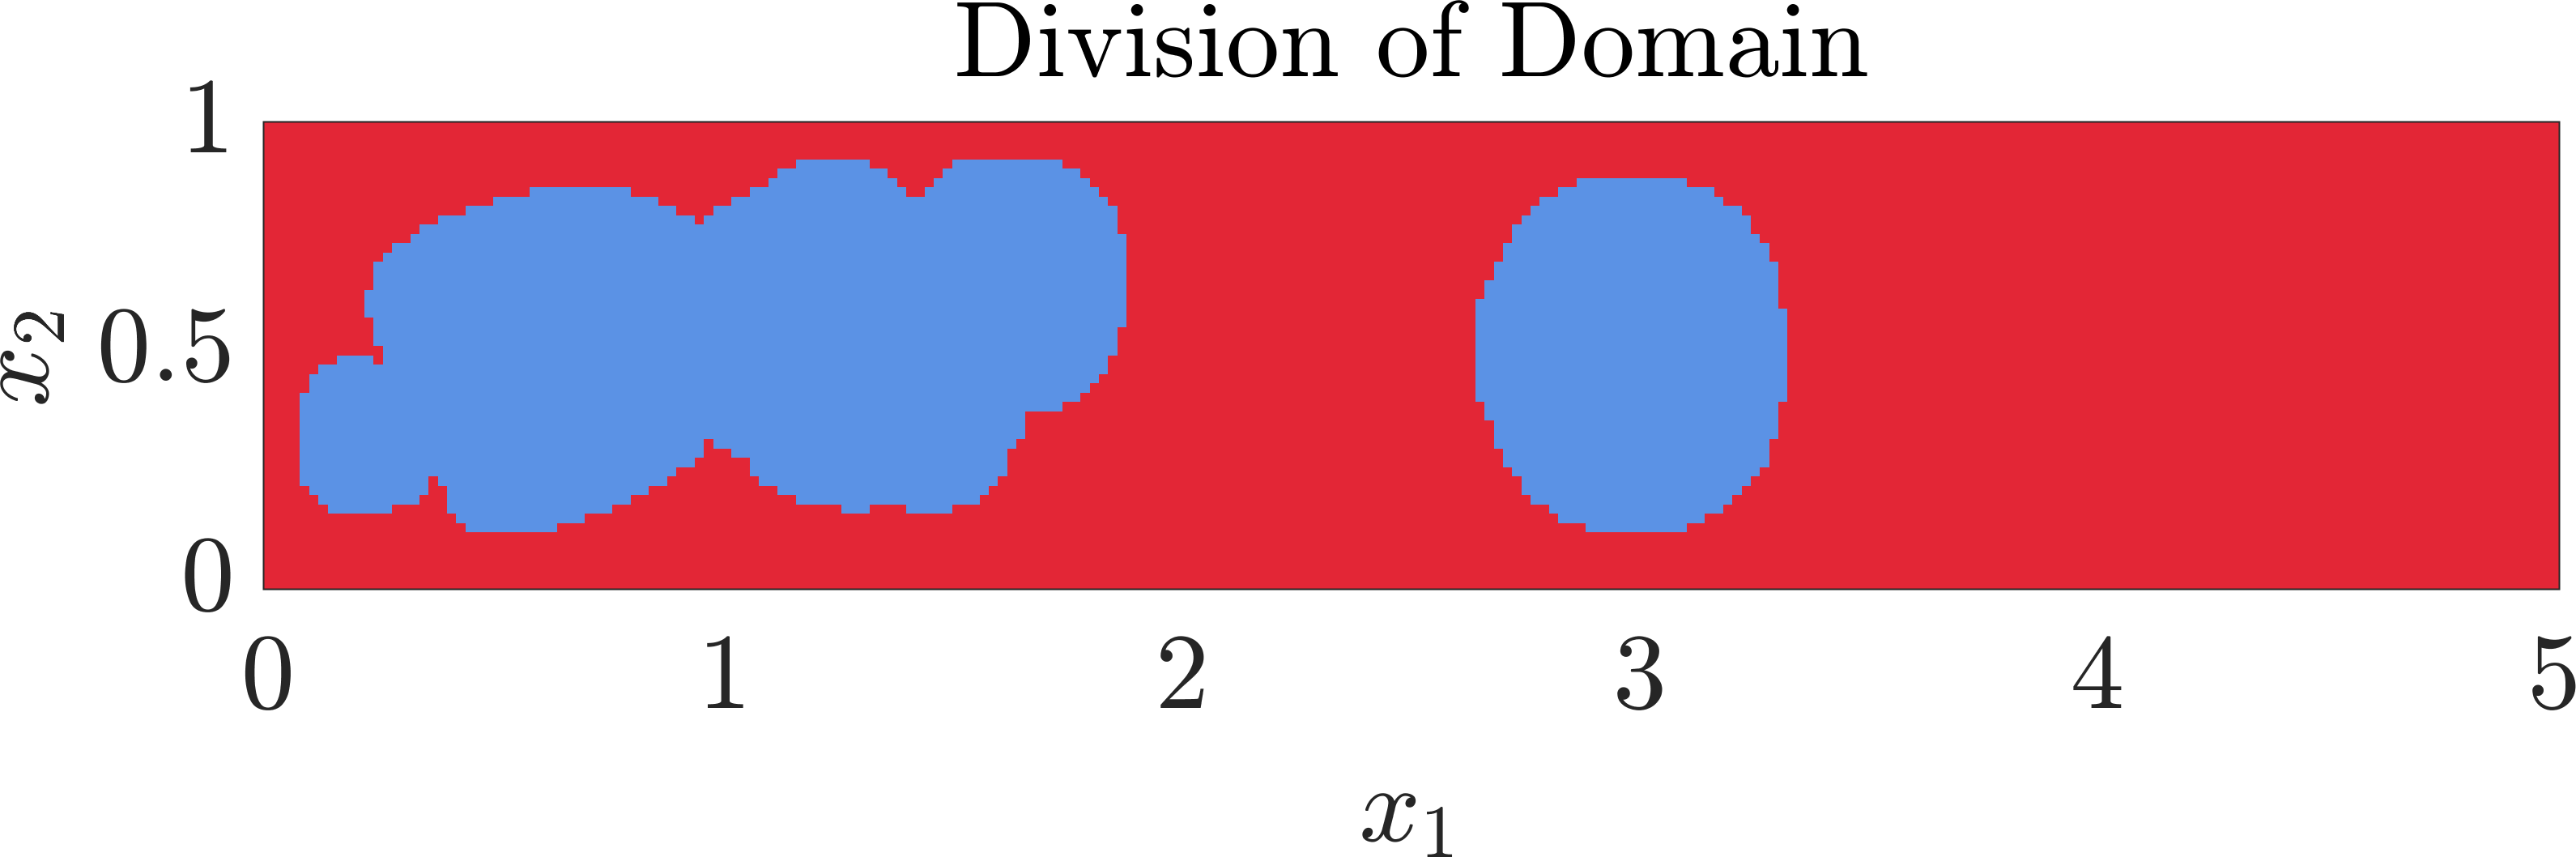
\includegraphics[width=0.48\textwidth]{svf/cd_cdr_MF03_divvy.png}
%  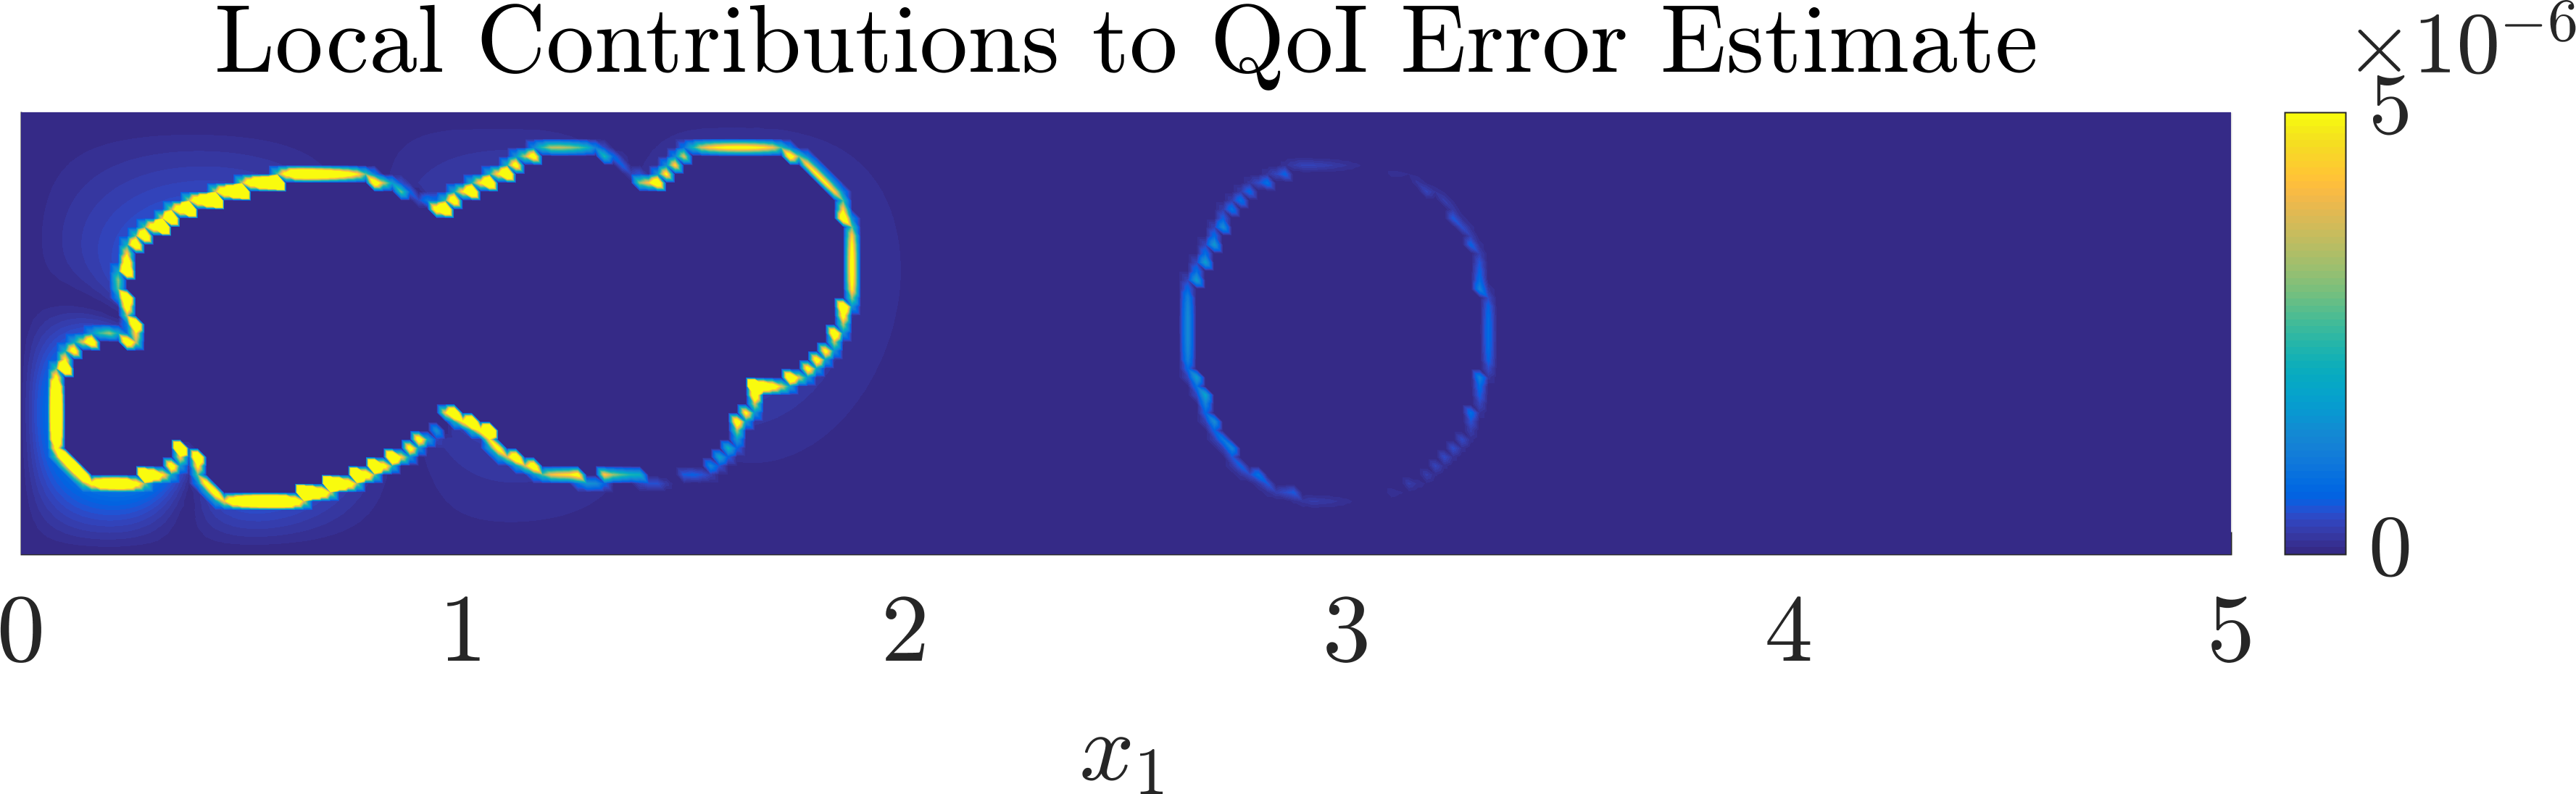
\includegraphics[width=0.51\textwidth]{svf/err_breakdown_MF03.png}
%  \vspace{-0.7\baselineskip}
%  \caption{MF$_3$ ($30\%$ HF)}
%  \vspace{0.8\baselineskip}
%\end{subfigure}
%\begin{subfigure}[b]{\textwidth}
%	\centering
%	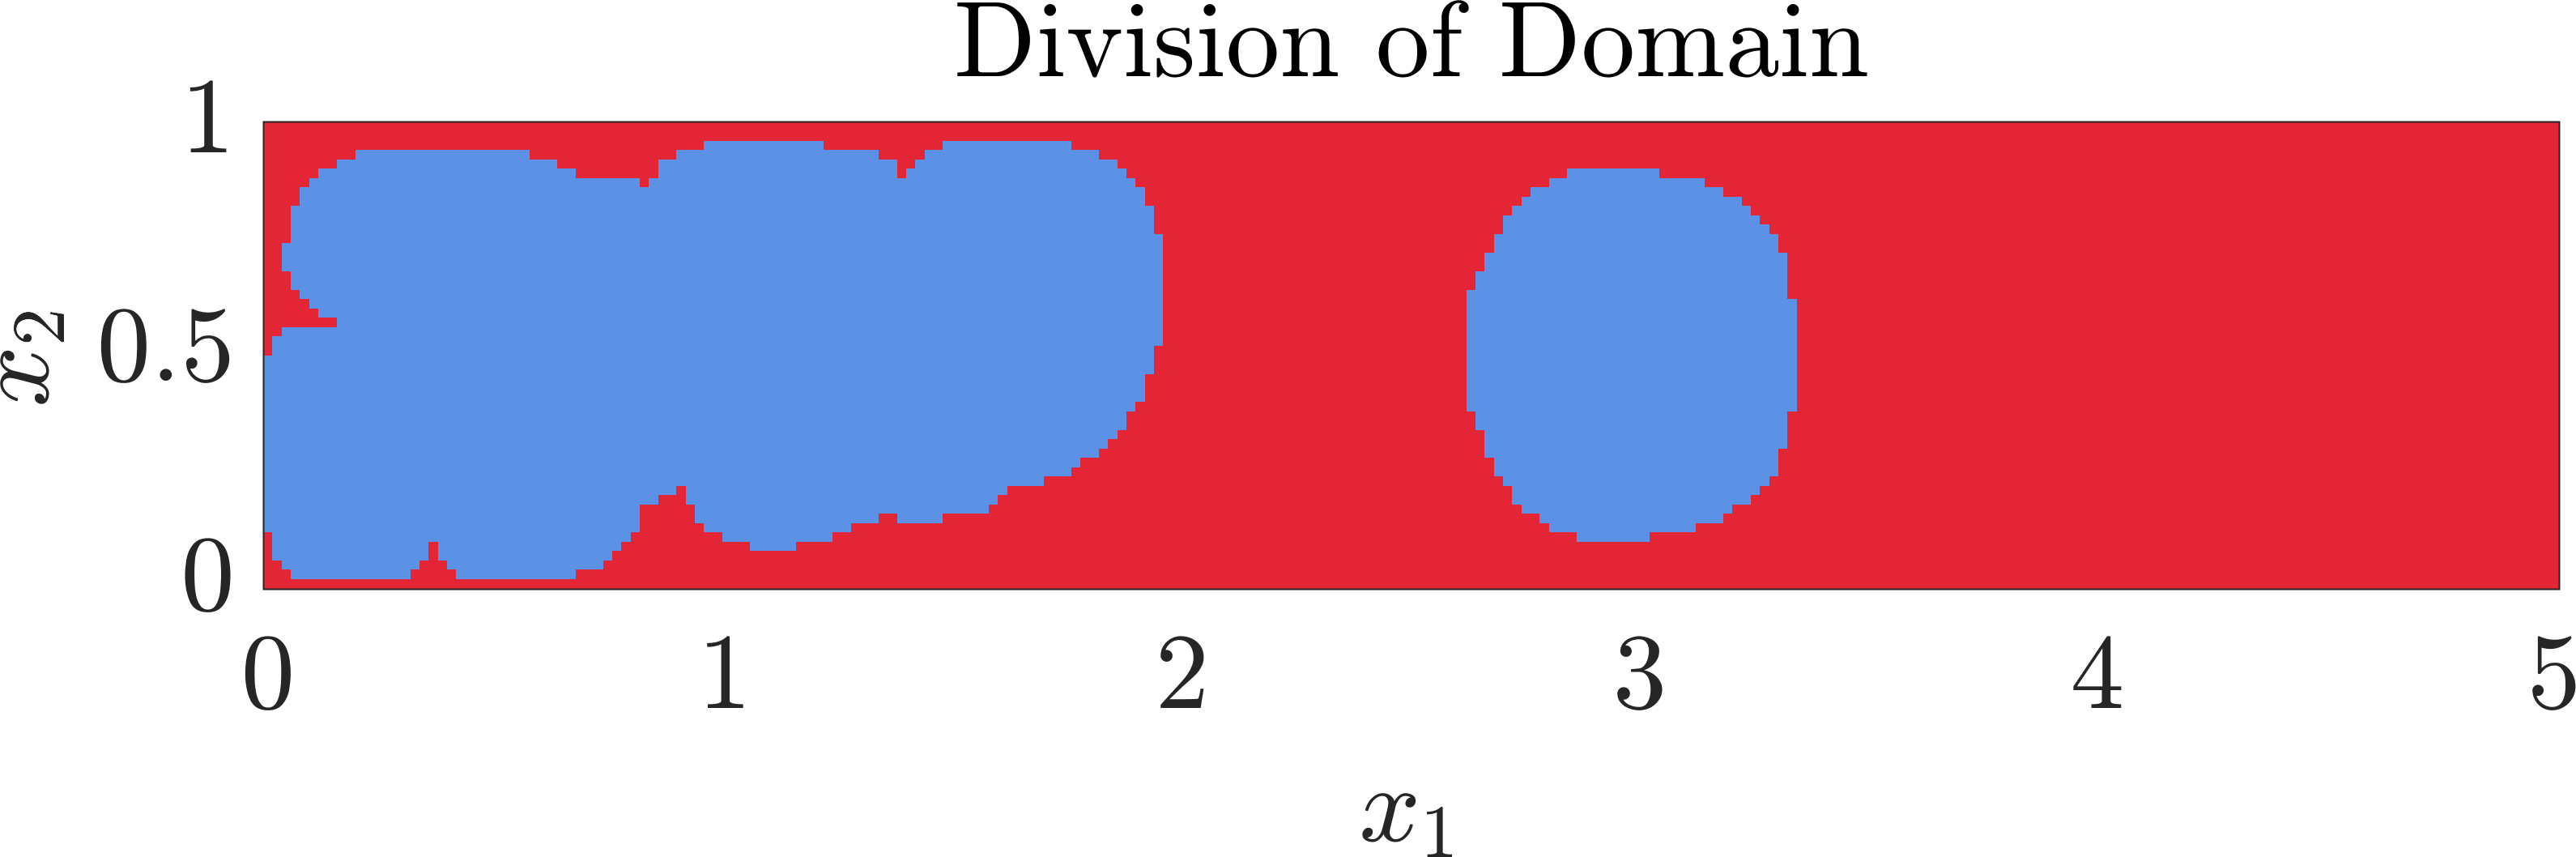
\includegraphics[width=0.48\textwidth]{svf/cd_cdr_MF04_divvy.png}
%  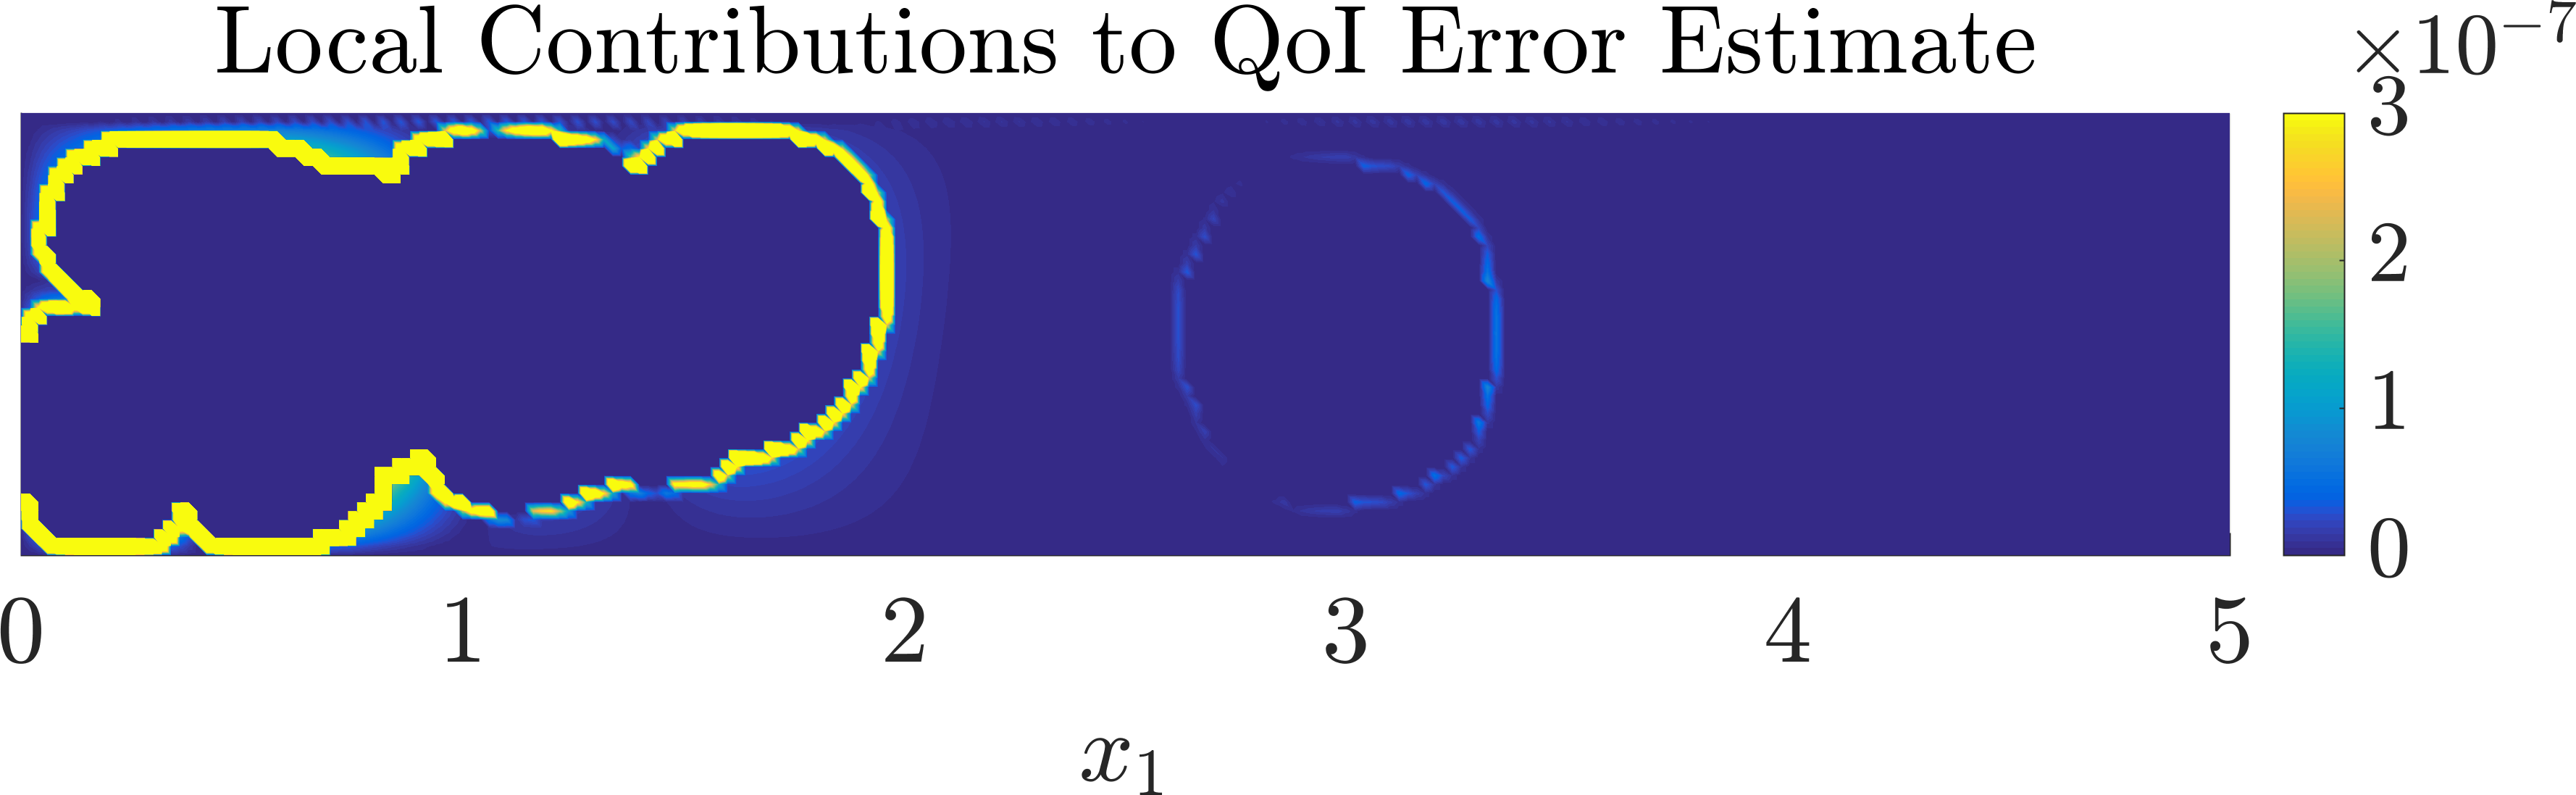
\includegraphics[width=0.51\textwidth]{svf/err_breakdown_MF04.png}
%  \vspace{-0.7\baselineskip}
%  \caption{MF$_4$ ($40\%$ HF)}
%  \vspace{0.8\baselineskip}
%\end{subfigure}
%\begin{subfigure}[b]{\textwidth}
%	\centering
%	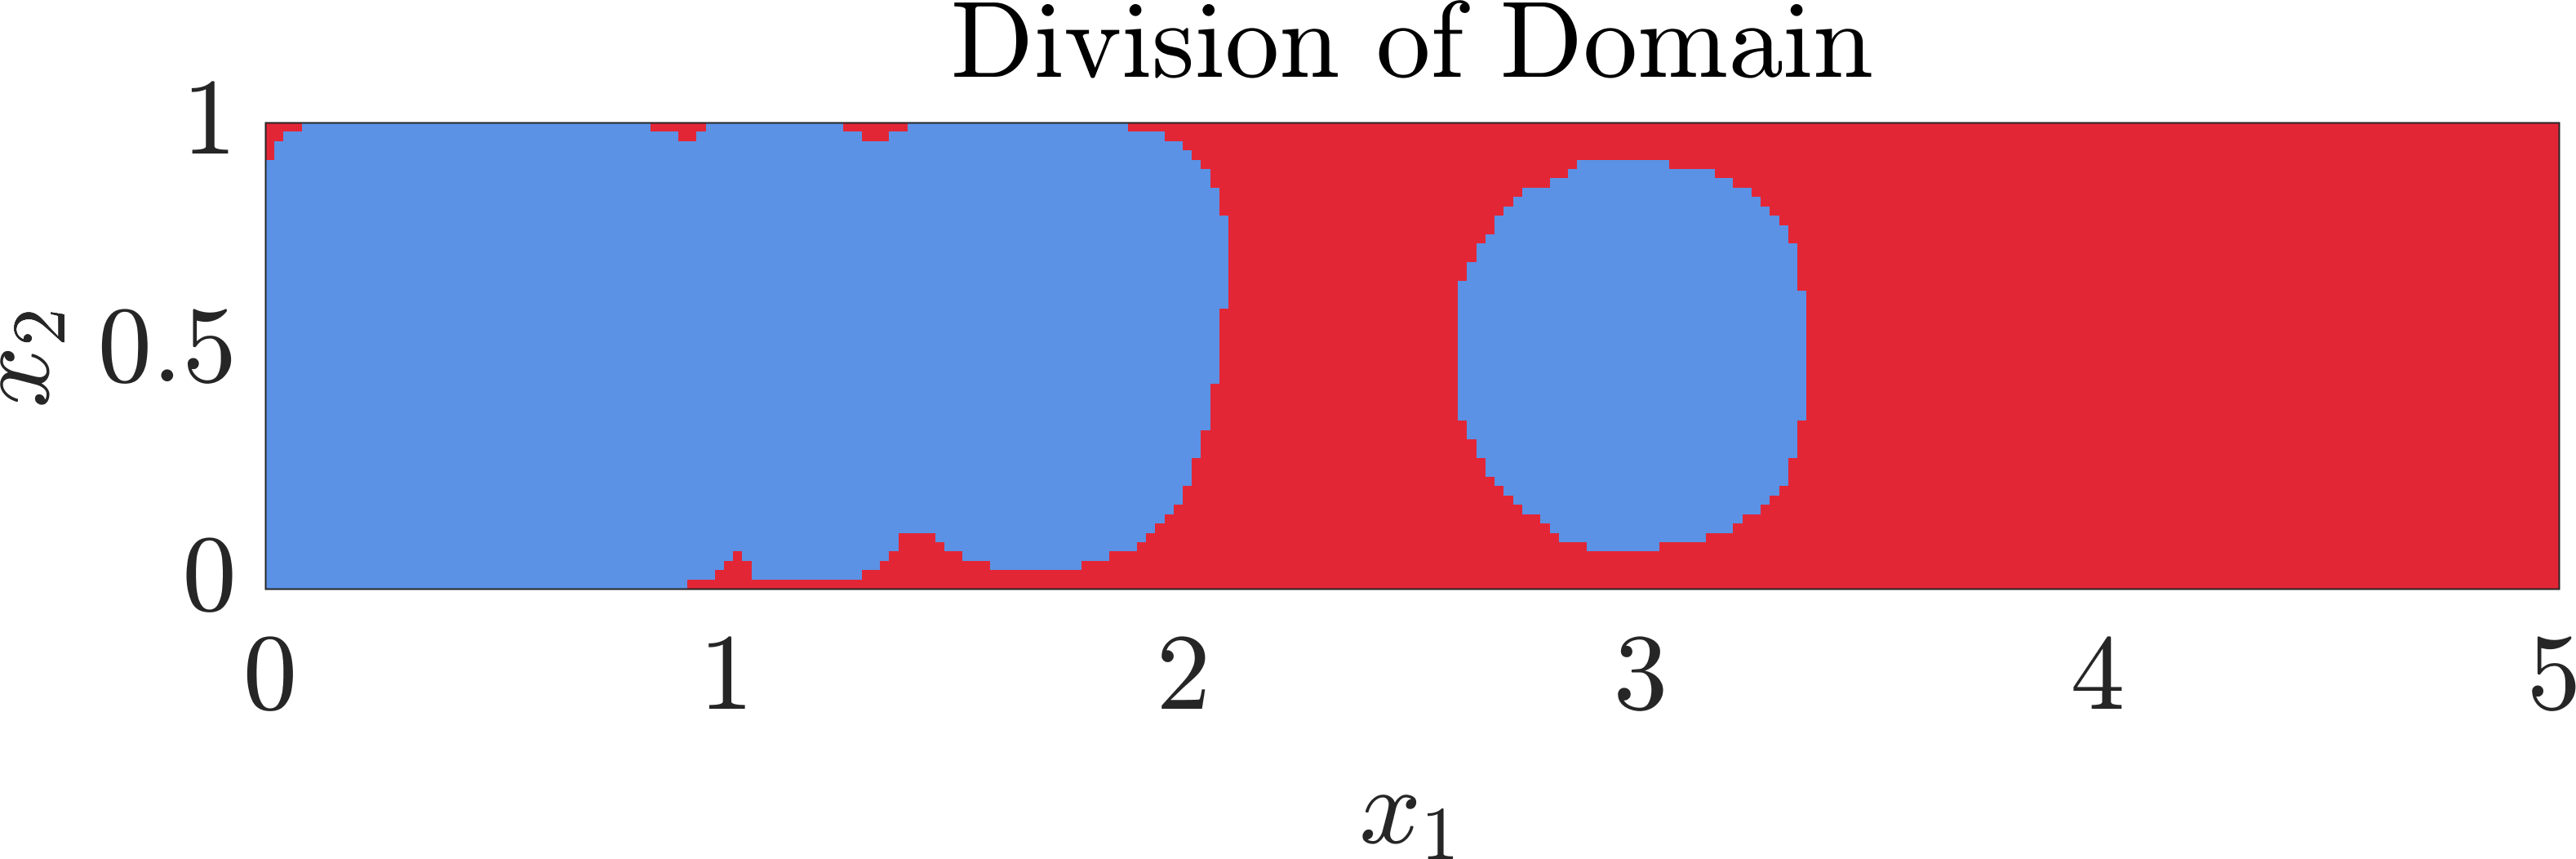
\includegraphics[width=0.48\textwidth]{svf/cd_cdr_MF05_divvy.png}
%  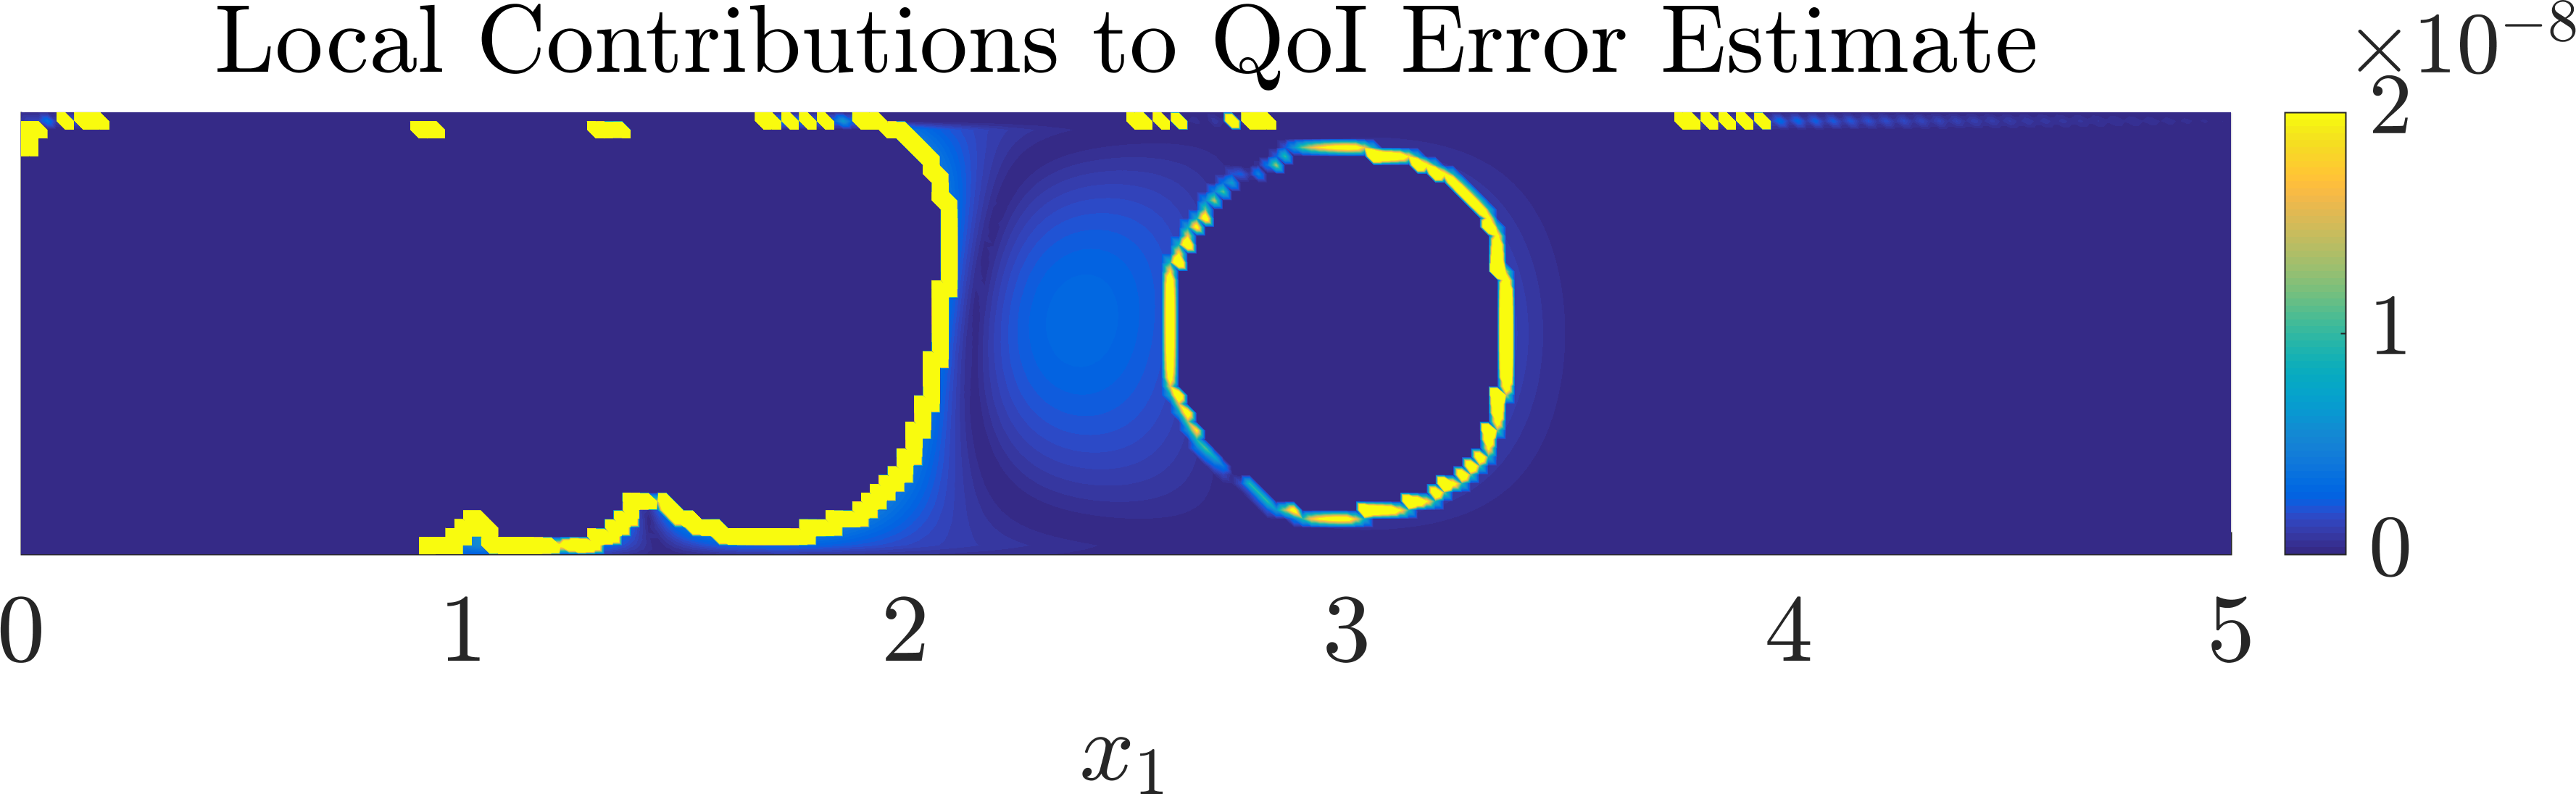
\includegraphics[width=0.51\textwidth]{svf/err_breakdown_MF05.png}
%  \vspace{-0.7\baselineskip}
%  \caption{MF$_5$ ($50\%$ HF)}
%  \vspace{0.8\baselineskip}
%\end{subfigure}
\subfloat[MF$_6$ ($60\%$ HF)]{
	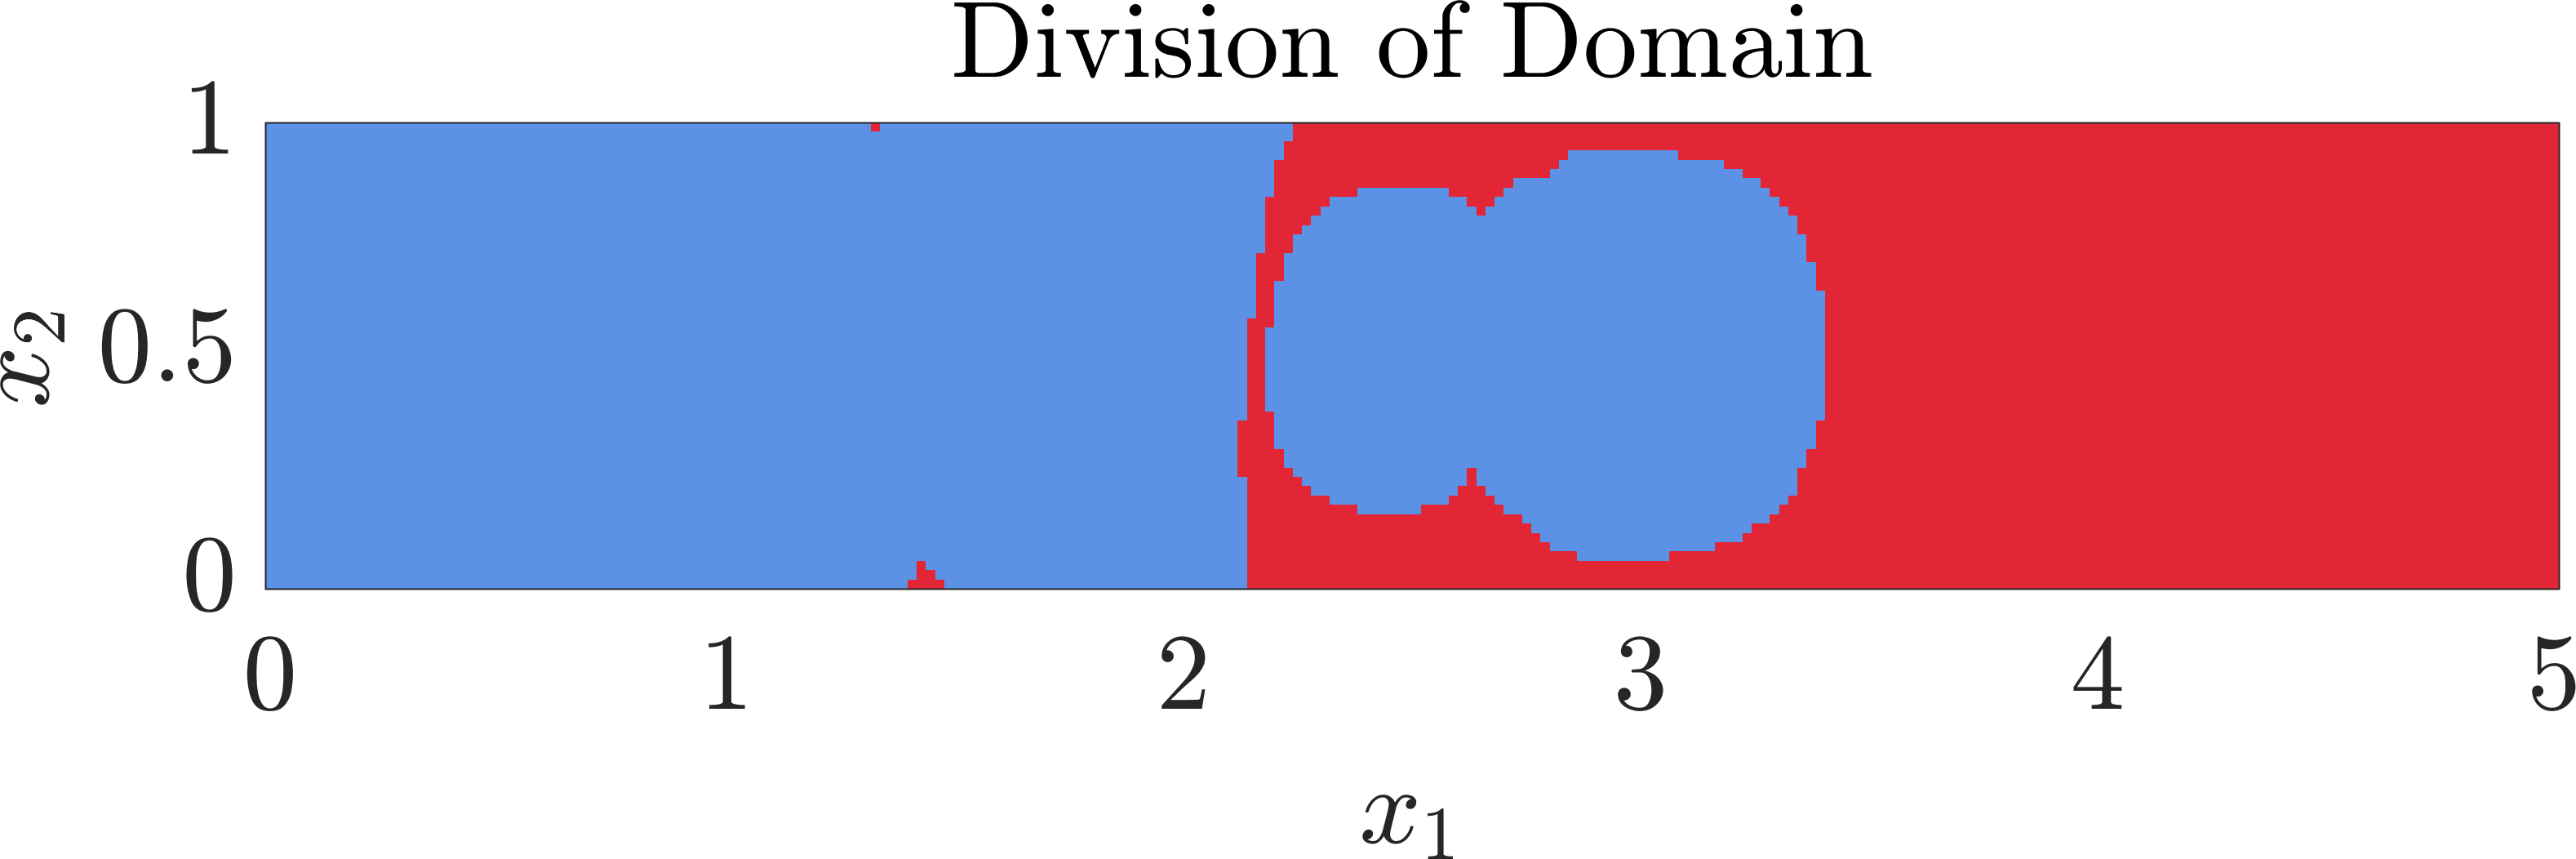
\includegraphics[width=0.46\textwidth]{svf/cd_cdr_MF06_divvy.png}
  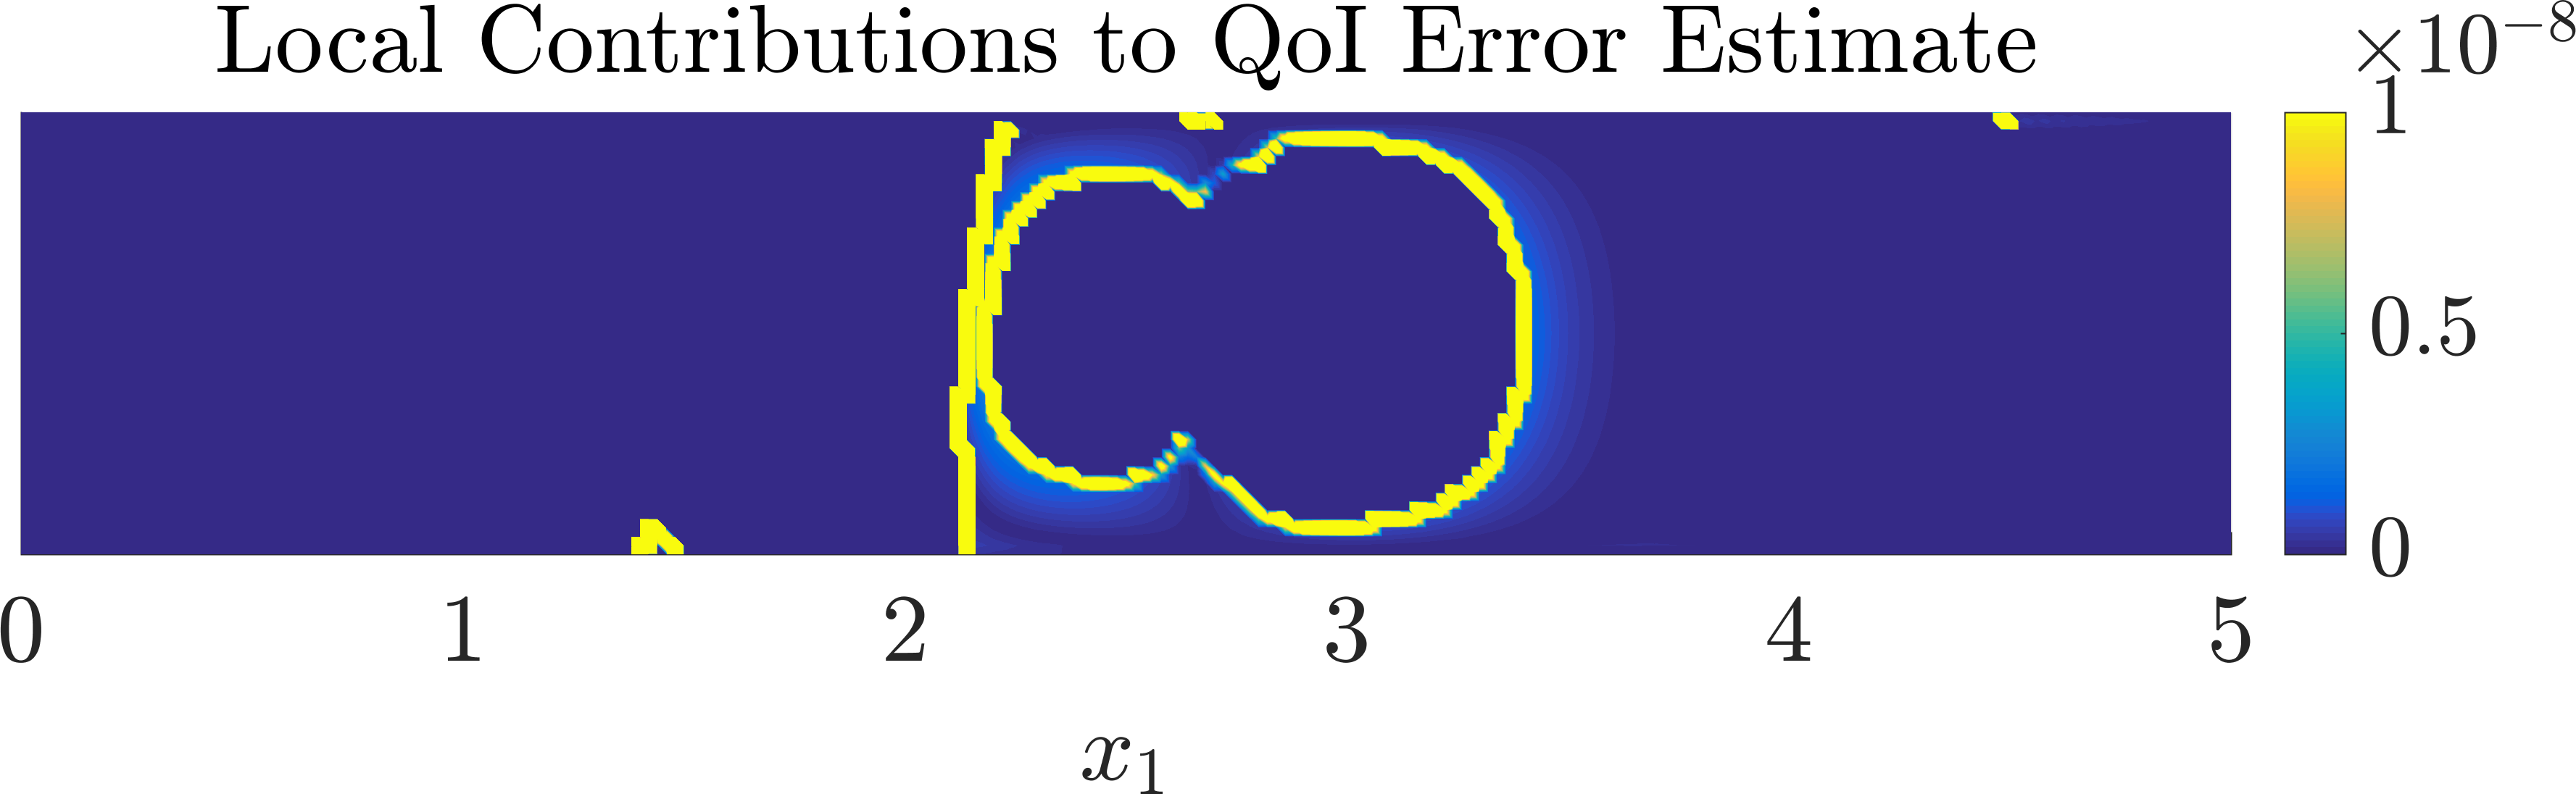
\includegraphics[width=0.49\textwidth]{svf/err_breakdown_MF06.png}
}
\caption{Left: Multi-fidelity refinement over the domain (low-fidelity constant-parameter model used in red portion, high-fidelity field-parameter model used in blue portion). Right: local error contributions. The (weighted) residual, and thus the local error contribution, tends to spike sharply at the interface between the low- and high-fidelity regions; the color range is truncated to make the error distribution visible elsewhere in the domain.}
\label{fig:svfRef}
\end{figure}
%
Comparing to \cref{fig:baseRef}, we see that in this case the local error contribution is not as greatly concentrated around the QoI region and the nearest \DIFdelbegin \DIFdel{data point}\DIFdelend \DIFaddbegin \DIFadd{observation location}\DIFaddend ; here, all three \DIFdelbegin \DIFdel{data points }\DIFdelend \DIFaddbegin \DIFadd{observation locations }\DIFaddend and the QoI region have associated regions of sufficiently similar high local error that all are refined in the first iteration. This reflects the global nature of the differences between the low- and high-fidelity models. 
%DIF <  KW: fix data-point language

The corresponding true and estimated absolute errors in the QoI are shown in \cref{fig:svfErr}.
%
\begin{figure}[htbp]
\centering
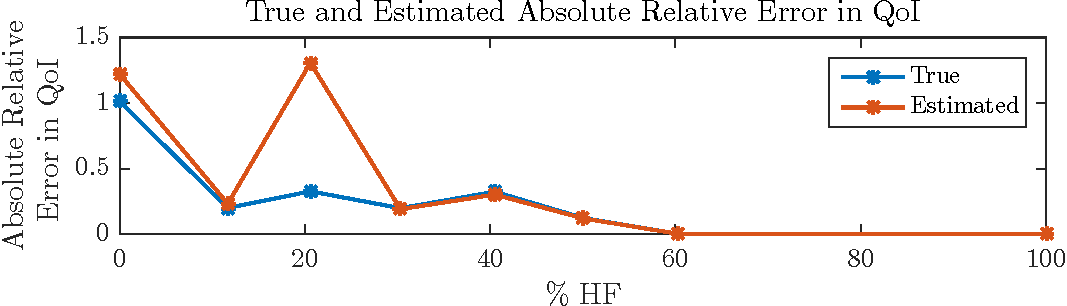
\includegraphics[width=0.8\textwidth]{svf/err_est.pdf}
\caption{True and estimated absolute relative error in QoI, plotted as a function of the percentage area of the domain in which the high-fidelity field-parameter model is used.}
\label{fig:svfErr}
\end{figure}
%
In this case, we see that we must use the high-fidelity model in most of the domain in order to get an accurate QoI. The adaptive algorithm requires us to use the field representation of the high-fidelity model in much of the left half of the domain; this reflects the topology of the inferred parameter field in the high-fidelity inverse problem, which is only relatively constant towards the right portion of the domain. We also see that in this case, in contrast to the example in \cref{sec:cdvcdrBaseRef}, increasing the proportion of the domain in which the high-fidelity model is used does not monotonically decrease the error in the QoI.

%------------------------------------------------------------------------------------------------------------------------%
\subsection{Combining Meshes and Physics in 3D} \label{sec:diffvcdr3D}
%------------------------------------------------------------------------------------------------------------------------%

In the previous examples, although the low- and high-fidelity models are sufficiently different to illustrate the behavior of \cref{alg:refSeries}, they are both simple enough and similar enough that using \cref{alg:refSeries} saves little, if any, computational effort. In this section, we consider a pair of models that differ in both the physics included and the mesh resolution, and we demonstrate computational savings using the multi-fidelity approach. In \cref{sec:setup3D_diffmesh} we describe the setup of the models and their inverse problems, and in \cref{sec:ref3D_diffmesh} we describe the results of applying \cref{alg:refSeries} to this pair of models.

%------------------------------------------------------------%
\subsubsection{Problem Setup} \label{sec:setup3D_diffmesh}
%------------------------------------------------------------%

The two models share a box domain $\Omega(x_1,x_2,x_3)$ which is $2300$m, $1650$m, and $100$m long in the $x_1$, $x_2$, and $x_3$ directions, respectively. We will refer to the positive and negative directions in $x_1$ as ``east" and ``west", respectively. The high-fidelity model is a single-species convection-diffusion-reaction equation with a nonlinear reaction term, described by
%
\begin{subequations}
\label{eq:cdvcdrHF3D}
\begin{align}
\nabla\cdot(n\vec{V}u - nD\nabla u) + k_ru^2 = f(q) \quad &\text{in } \Omega, \label{eq:HFeq3D}\\
u = 0 \quad &\text{on } \partial \Omega_{west}, \\
\frac{\partial u}{\partial n} = 0 \quad &\text{on }\partial\Omega_{east}, \\
\hat{n}\cdot(n\vec{V}u - nD\nabla u) = 0 \quad &\text{on }\partial\Omega\backslash(\partial\Omega_{east}\cup\partial\Omega_{west}),
\end{align}
\end{subequations}
%
where the state $u$ is the mass-fraction (in parts-per-billion) of some contaminant species and $f(q)$ is a source/sink field. The velocity field is a constant $\vec{V}=(2.1,0,0)$ m/day. Given this velocity field and letting the molecular diffusion be \DIFdelbegin \DIFdel{negligble}\DIFdelend \DIFaddbegin \DIFadd{negligible}\DIFaddend , we follow \cite{Vestedetal93} to express the (diagonal) dispersion tensor $D$ as $D_{11}=\alpha_{LH}V_1$, $D_{22}=\alpha_{TH}V_1$, and $D_{33}=\alpha_{TV}V_1$, where $\alpha_{LH}=100$m, $\alpha_{TH}=40$m, and $\alpha_{TV}=4$m are the longitudinal horizontal, transverse horizontal, and transverse vertical dispersivities, respectively; the dispersivity values were drawn from within the range of observed values in various porous media \cite{Davis86}. We have porosity $n=0.1$. The reaction coefficient is $k_r=4.2\cdot10^{-4}$ 1/day, chosen from within the wide range of reaction-rate coefficients for second-order reactions. Although the reaction term $k_ru^2$ does not correspond to any particular reaction of any particular species, we note that, in addition to second-order elementary reactions, a quadratic reaction term can appear in models of dissolution/precipitation processes in porous media \cite{Aha97} and biochemical \DIFdelbegin \DIFdel{degredation }\DIFdelend \DIFaddbegin \DIFadd{degradation }\DIFaddend of petroleum hydrocarbons in soils \cite{Jack94}.

The low-fidelity model,
%
\begin{equation}
\nabla\cdot(- nk_d\nabla u) = f(q) \quad \text{in } \Omega, \label{eq:LFeq3D}
\end{equation}
%
differs in the removal of the reaction and convection terms and the anisotropy of the dispersion tensor; the dispersion tensor $D$ is replaced with a scalar $k_d=D_{11}$. The boundary conditions remain unchanged. As in the previous examples in \cref{sec:cdvcdr}, the mixed-fidelity models are formed by dividing the domain into complementary subdomains $\Omega_{HF}$ and $\Omega_{LF}$, where \cref{eq:HFeq3D,eq:LFeq3D} are solved, respectively. The QoI we wish to calculate is the integral of the state over a region $\Omega_I$.

The unknown parameters we wish to infer correspond to the source term $f(q)=q$; we impose $f(q)=q=0$ on the boundary $\partial\Omega$. Synthetic observations at 18 points in the domain are generated by running the high-fidelity model on a finer mesh. The locations of the observations as well as the QoI region $\Omega_I$ are shown in \cref{fig:setup3D}. We \DIFdelbegin \DIFdel{use a regularization term $\frac{\beta}{2}\int_\Omega \|\nabla f(q)\|_2^2\:\textrm{d}V$.
%DIF <  KW: again please connect reg term to an equation or just state objective function here.
}\DIFdelend \DIFaddbegin \DIFadd{set the regularization term in }\cref{eq:invOpt_obj} \DIFadd{to be $R(q)=\frac{\beta}{2}\int_\Omega \|\nabla f(q)\|_2^2\:\textrm{d}V$.
}\DIFaddend %
\begin{figure}[htbp]
\centering
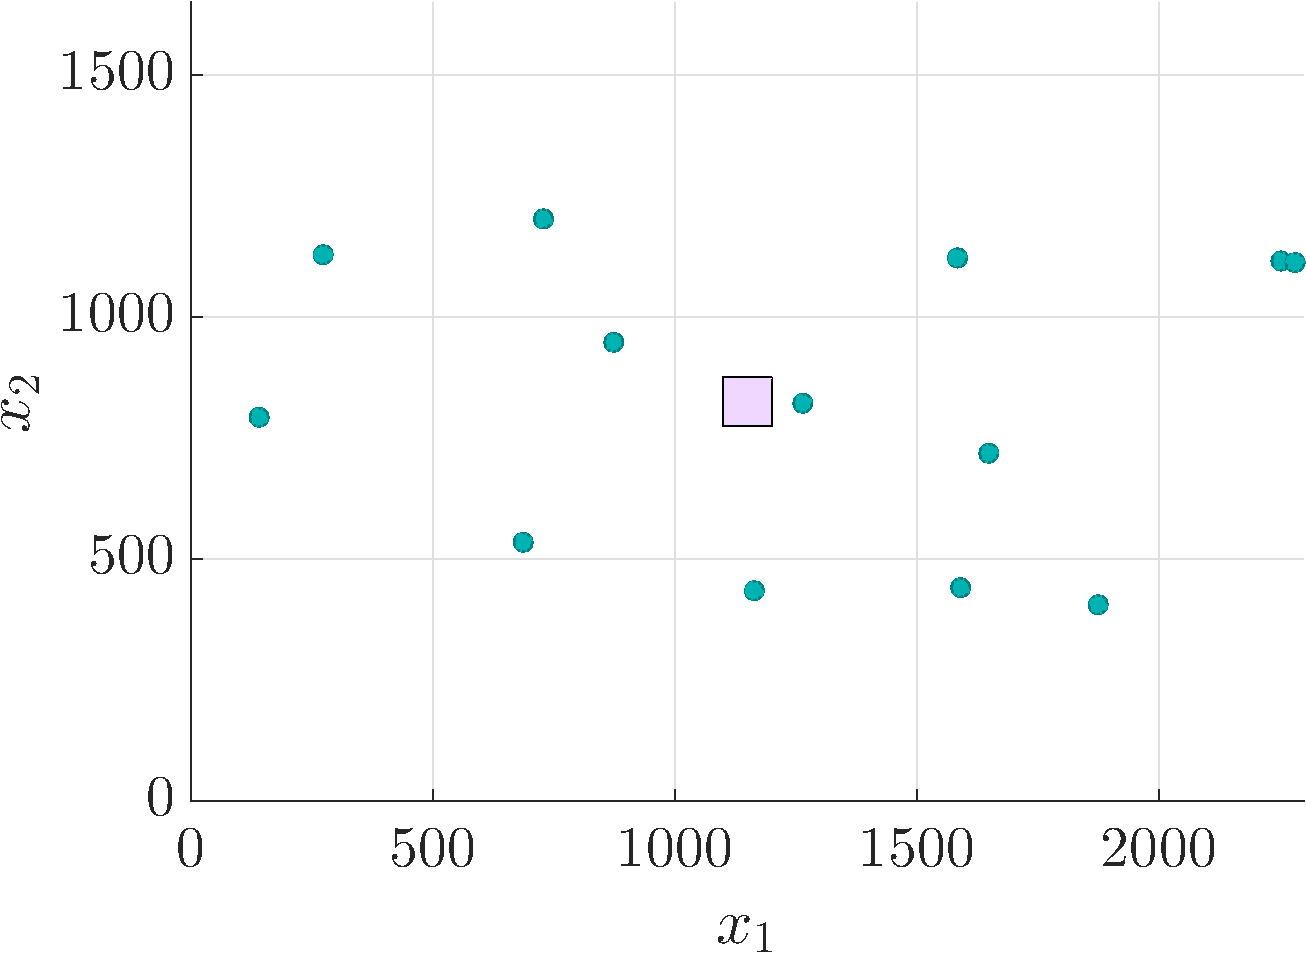
\includegraphics[width=0.4\textwidth]{series3D/setup_aerial_nolegend.pdf} \hfill
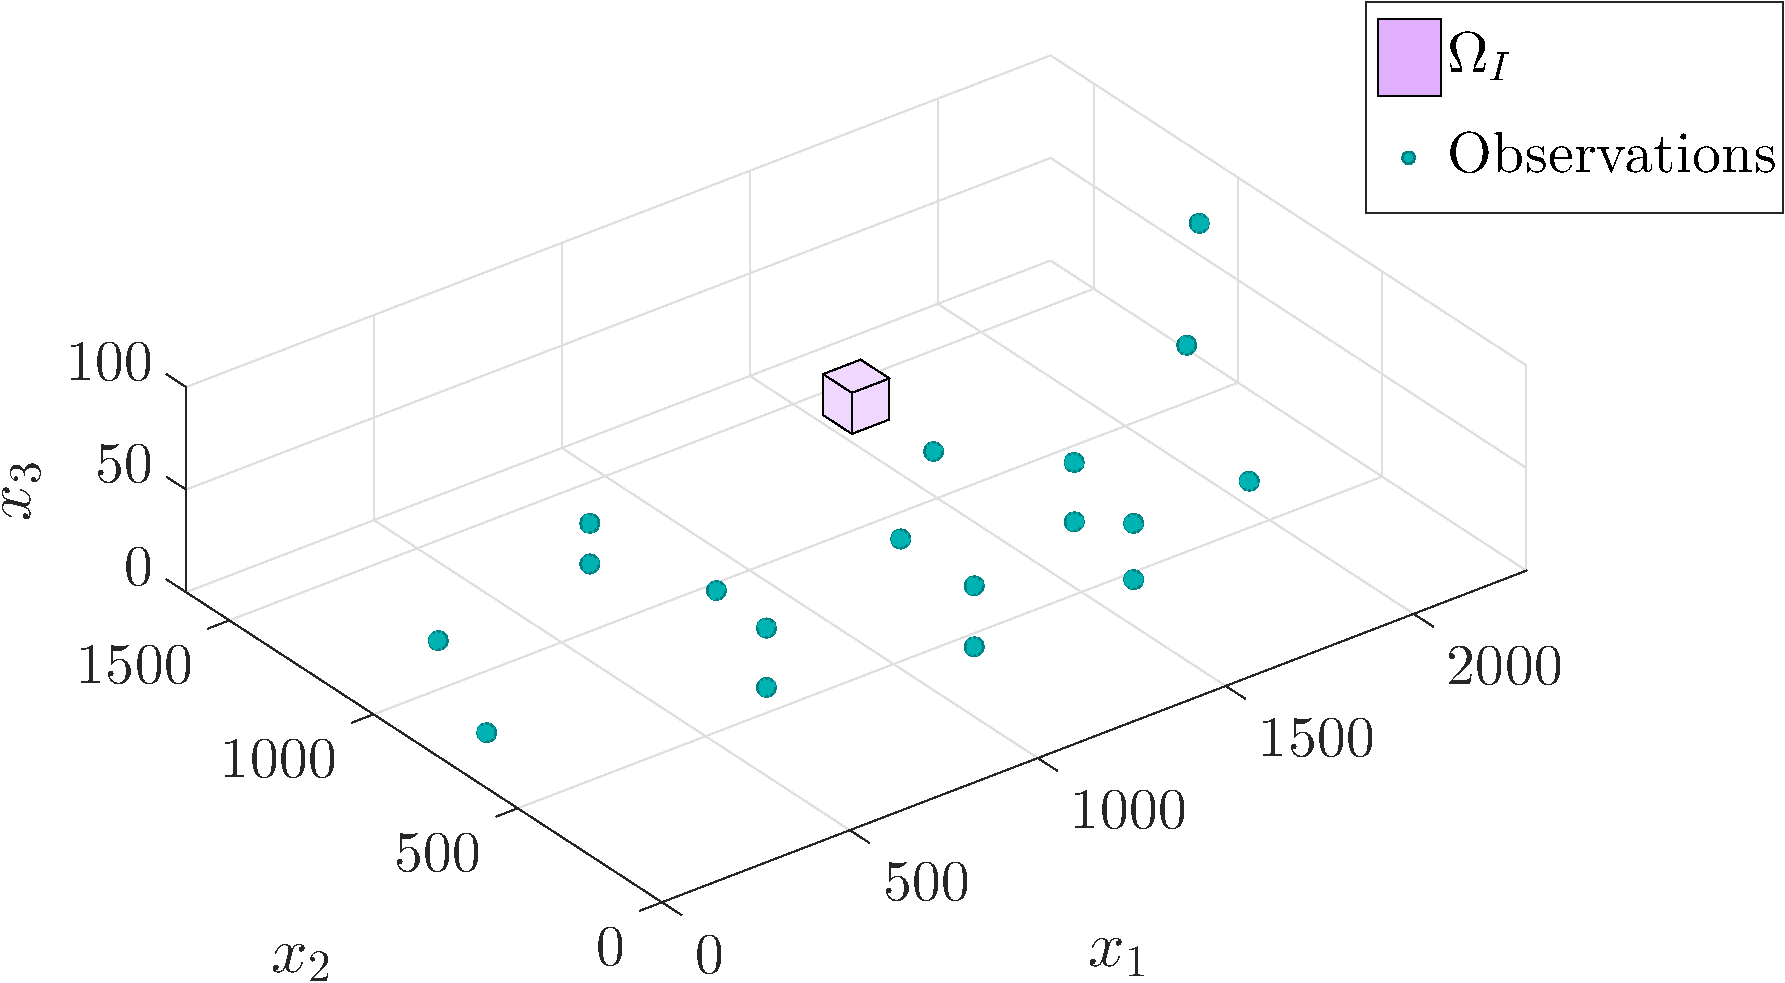
\includegraphics[width=0.55\textwidth]{series3D/setup_3view.pdf} \\
\vspace{\baselineskip}
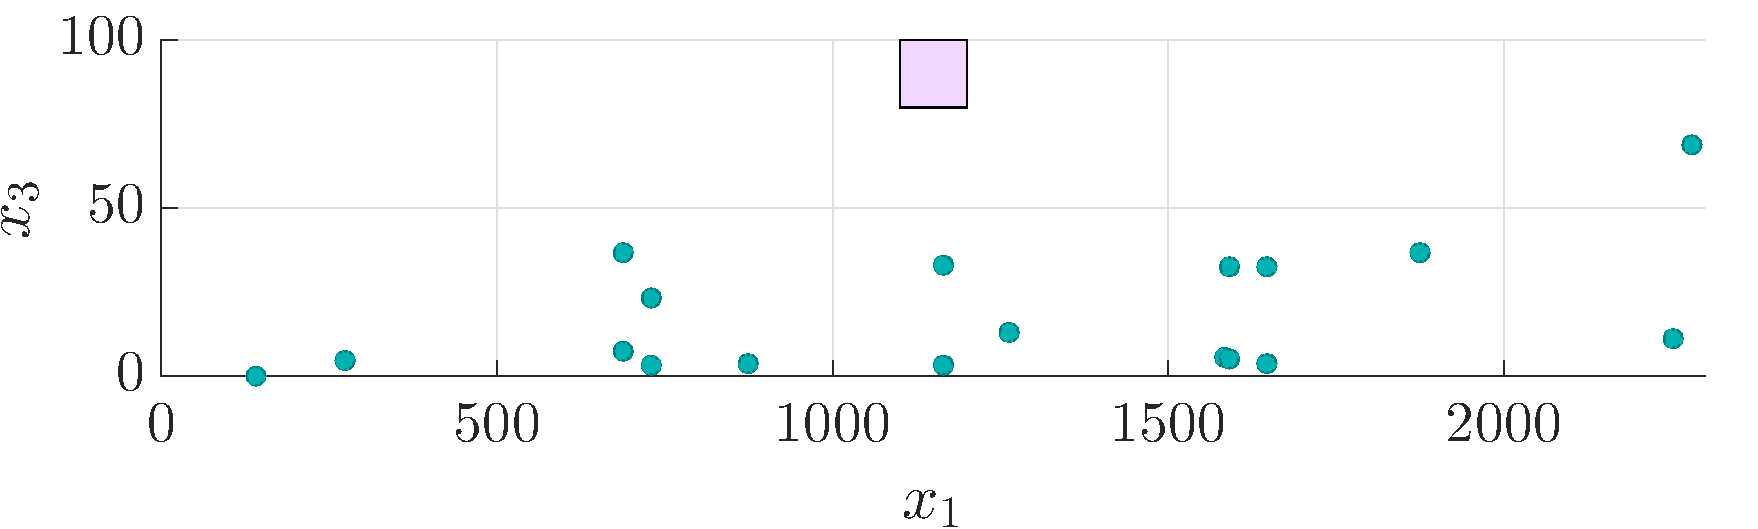
\includegraphics[width=0.6\textwidth]{series3D/setup_side_view.pdf}
\caption{Three views of the locations of the observations and the QoI region.}
\label{fig:setup3D}
\end{figure}
%

We use a FEM with a continuous Galerkin formulation and Lagrange elements. The lack of a convection term allows the low-fidelity model to be solved on a coarser mesh. For the high-fidelity model, the domain is discretized by 32, 64, and 32 elements along the $x_1$, $x_2$, and $x_3$ directions, respectively; for the low-fidelity model, the domain is discretized by 16, 32, and 16 elements along the $x_1$, $x_2$, and $x_3$ directions, respectively. The cell P\'{e}clet number is less than one and so stabilization is not required.

%------------------------------------------------------------%
\subsubsection{Adaptive Model Refinement Results} \label{sec:ref3D_diffmesh}
%------------------------------------------------------------%

We now present the results of solving the inference problem using \cref{alg:refSeries}, with a relative error tolerance of $0.1\%$. At each iteration, we choose the $2\%$ of the basis functions with the largest error for model refinement; since each linear Lagrange basis function has eight elements in its support, the number of additional elements marked for refinement in each iteration is usually greater than for the 2D examples. All simulations are run on a single processor; we use the default nonlinear solver in \texttt{libMesh} \DIFaddbegin \DIFadd{\cite{libMeshPaper} }\DIFaddend (Newton's method with Brent line-search), and linear solves are performed using \DIFdelbegin \DIFdel{PETSC's }\DIFdelend \DIFaddbegin \DIFadd{PETSc's \cite{petsc-user-ref} }\DIFaddend GMRES solver, preconditioned by incomplete factorization.
%DIF <  KW: need to add a citation to papers for libMesh and PETSC?

\Cref{tab:ref3D_diffmesh} shows the error at the end of each adaptive iteration. Each iteration of the adaptive algorithm uses the solution of the previous iteration as its initial guess. The number of degrees of freedom of each of the primary (and, if applicable, auxiliary) variables at each iteration is also given; the supplementary adjoint is solved on the high-fidelity mesh and thus each of its variables has the same number of degrees of freedom as each of the primary variables in the high-fidelity inverse problem. The high-fidelity inverse problem does not converge when the low-fidelity solution is used as an initial guess. Instead, we solve the inverse problem for an intermediate model
%
\begin{equation}
\nabla\cdot(n\vec{V}u - nD\nabla u) + k_ru^2 = f(q)
\end{equation}
%
and use the solution as an initial guess for the high-fidelity problem; equivalently, we use two steps of natural continuation on the reaction parameter: $k_r=0$, then $k_r=4.2\cdot10^{-4}$.
%
\begin{table}[htbp]
\caption{Runtime and relative errors of adaptive algorithm iterations given relative error tolerance of $0.1\%$; relative errors are given with respect to the high-fidelity QoI estimate.}
\label{tab:ref3D_diffmesh}
\centering
\begin{tabular}{|c|c|c|c|c|c|c|c|c|}
\hline
\multirow{2}{*}{Case} & \multirow{2}{*}{$\%$HF} & \multirow{2}{*}{DOFs} & \multirow{2}{*}{QoI} & Error & Error & $\%$ Relative \\
& & & & (Estimated) & (Actual) & Error (Actual)  \\ \hline
LF   & 0    & 9537  & 168710 & -16463 & -85663 & -103    \\
MF01 & 5.2  & 13417 & 167366 & -7207  & -84319 & -102    \\
MF02 & 11.4 & 17895 & 89777  & -6208  & -6730  & -8.10   \\
MF03 & 16.3 & 21001 & 85880  & -2473  & -2833  & -3.41   \\
MF04 & 22.0 & 24528 & 83902  & -711   & -855   & -1.03   \\
MF05 & 27.7 & 27984 & 83119  & 32     & -72    & -0.087  \\
HF   & 100  & 70785 & 83047  & --     & --     & --    \\ \hline
\end{tabular}
\end{table}
%

We notice that, compared to the results in \cref{fig:baseErr}, the error estimates for the low-fidelity and first mixed-fidelity models are far from the true errors. This can be attributed to the linearization about $\Psi_{LF}$ and $\Psi_{MF_{1}}$ instead of $\Psi_{HF}$ in solving the supplementary adjoints \DIFaddbegin \DIFadd{as well as the third-order term that is ignored in the error estimate}\DIFaddend ; the large differences in the QoI for the LF and MF01 models compared to the high-fidelity QoI indicate that $\Psi_{LF}$ and $\Psi_{MF_{1}}$ are significantly different from $\Psi_{HF}$. Compared to the pair of models in \cref{sec:cdvcdrSetup}, the low- and high-fidelity models \DIFaddbegin \DIFadd{in this case }\DIFaddend are more dissimilar, even though \DIFaddbegin \DIFadd{in both }\cref{sec:cdvcdrSetup} \DIFadd{and this case }\DIFaddend the nonlinear term in the high-fidelity \DIFdelbegin \DIFdel{models remain the same. }\DIFdelend \DIFaddbegin \DIFadd{model }\cref{eq:cdvcdrHF} \DIFadd{and }\cref{eq:cdvcdrHF3D} \DIFadd{is a quadratic reaction term. }\DIFaddend % KW: don't know what last part of this sentence means. what hi-fi models?
\DIFdelbegin \DIFdel{This behavior suggests that one should use more than just the error estimate to decide when to stop the adaptive algorithm; a possible additional criterion could be to require that the predicted high-fidelity QoI $I(q_{MF},u_{MF})+\epsilon_i$ for two consecutive iterations agree to within some tolerance. %DIF <  KW: what behavior? this last sentence doesn't follow from the previous one. and what predicted hi-fi QOI? Do you mean mixed-fi? I'm not sure this is a good idea. I'd probably delete this last sentence.
}\DIFdelend %DIF > The possibility of large inaccuracies in the error estimates of low-fidelity and mostly unrefined mixed-fidelity models suggests that one should use more than just the error estimate to decide when to stop the adaptive algorithm; a possible additional criterion could be to require that the estimated high-fidelity QoI ($I(q_{MF},u_{MF})+\epsilon_i$) for two consecutive iterations agree to within some tolerance. % KW: what behavior? this last sentence doesn't follow from the previous one. and what predicted hi-fi QOI? Do you mean mixed-fi? I'm not sure this is a good idea. I'd probably delete this last sentence.
%DIF >  or just let the reader decide how to deal with possibly inaccurate initial error estimates?

The multi-fidelity domain refinements for the five adaptive iterations are shown in \cref{fig:divvy3D_diffmesh}. Similarly to the behavior seen in \cref{sec:cdvcdrBaseRef}, the QoI region and the areas around some of the measurement points are first targeted for refinement, with those measurement points furthest downstream of the QoI being the last to receive refinement. We also see that the domain is refined completely in the $x_3$ direction first around the QoI region, reflecting the large difference in the high-fidelity dispersion tensor $D$ and the low-fidelity dispersion coefficient in the $x_3$ direction.
%
\begin{figure}[htbp]
\centering
\subfloat[MF$_1$ ($5.2\%$ HF)]{
\includegraphics[width=0.31\textwidth]{series3D/run_diff_mesh/divvy1_whitebg_puff.png}
}
\subfloat[MF$_2$ ($11.4\%$ HF)]{
\includegraphics[width=0.31\textwidth]{series3D/run_diff_mesh/divvy2_whitebg_puff.png}
}
\subfloat[MF$_3$ ($16.3\%$ HF)]{
\includegraphics[width=0.31\textwidth]{series3D/run_diff_mesh/divvy3_whitebg_puff.png}
} \\
\subfloat[MF$_4$ ($22.0\%$ HF)]{
\includegraphics[width=0.31\textwidth]{series3D/run_diff_mesh/divvy4_whitebg_puff.png}
}
\subfloat[MF$_5$ ($27.7\%$ HF)]{
\includegraphics[width=0.31\textwidth]{series3D/run_diff_mesh/divvy5_whitebg_puff.png}
}
\caption{Domain division for mixed-fidelity models: low-fidelity convection-diffusion model used in red portion, high-fidelity convection-diffusion-reaction model used in blue portion (intermediate colors due to transparency indicate a mix of the two models along the line of sight); $x_3$ direction scaled for clarity.}
\label{fig:divvy3D_diffmesh}
\end{figure}
%

In this case, although the mixed-fidelity models have fewer degrees of freedom than the high-fidelity model, it is faster to solve the high-fidelity inverse problem than to adaptively seek a mixed-fidelity model with a small QoI error, starting from the low-fidelity model. This can be attributed to multiple factors: the high-fidelity problem is mildly nonlinear and has a close initial guess that is a solution to a linear system (when $k_r=0$), and the supplementary adjoint is solved on the high-fidelity mesh. Generally, as the nonlinearity of the high-fidelity model increases, one would expect solving the high-fidelity inverse problem to require more time relative to using the adaptive algorithm. However, one can also consider an ``offline-online" setting, where the mixed-fidelity models are identified up-front by applying \Cref{alg:refSeries} to a set of representative observations $d^*$. Then when actual/new data are received, one can solve the inverse problem with the mixed-fidelity model and the new data, and, if desired, compute an updated error estimate for the QoI. The mixed-fidelity inverse problems are expected to require less time to solve than the high-fidelity inverse problems.

To illustrate this offline-online application, we generate ten sets of noisy observations to represent the actual data gained during the online phase; the noisy observations are generated by taking the observations used in the adaptive algorithm and adding Gaussian white noise with standard deviation of $\sigma=0.02$ (equivalent to, on average, $5\%$ of the observed values). We then solve the inverse problem using each of the mixed-fidelity models depicted in \cref{tab:ref3D_diffmesh,fig:divvy3D_diffmesh} as well as the high-fidelity model. The low-fidelity inverse problem is first solved and used as an initial guess for the higher-fidelity problems; we note that although there is a linear model that is more similar to the high-fidelity model than the low-fidelity model (i.e., convection-diffusion with anisotropic diffusivity and $k_r=0$ on the high-fidelity mesh) and thus would serve as a better initial guess, its existence is specific to our particular choice of models. The auxiliary and supplementary adjoint variables use a zero initial guess.

\Cref{tab:ref3D_newdata_QoI_diffmesh} shows the average QoI values, error estimates and solution times for the (non)linear solves. \Cref{tab:ref3D_newdata_times_diffmesh} shows the times needed to solve the inverse problems and to solve for the additional variables needed to obtain an error estimate. For six of the ten datasets, the high-fidelity inverse problem does not converge given the low-fidelity solution as an initial guess; these are solved using the $k_r=0$ solution as an initial guess so that true QoI errors can be calculated. The average high-fidelity inverse problem solution time shown in \cref{tab:ref3D_newdata_times_diffmesh} includes only those cases (four of ten) that converged with the low-fidelity initial guess.
%
\begin{table}
\caption{Average QoI values and errors from solving inverse problem with mixed- and high-fidelity models and noisy data; relative errors are with respect to true high-fidelity QoI.}
\label{tab:ref3D_newdata_QoI_diffmesh}
\centering
\begin{tabular}{|c|c|c|c|c|c|}
\hline
\multirow{2}{*}{Case} & \multirow{2}{*}{$\%$HF} & \multirow{2}{*}{QoI} & Error & Error & $\%$ Relative  \\
& & & (Estimated) & (Actual) & Error (Actual) \\ \hline
LF   & 0    & 166774 & --    & -84326 & -102.3 \\
MF01 & 5.2  & 164597 & 4347  & -82149 & -99.65  \\
MF02 & 11.4 & 88867  & -5921 & -6418  & -7.79  \\
MF03 & 16.3 & 85237  & -2414 & -2789  & -3.38  \\
MF04 & 22.0 & 83411  & -724  & -963   & -1.17  \\
MF05 & 27.7 & 82664  & -18   & -216   & -0.26 \\
HF   & 100  & 82500  & --    & --     & --  \\ \hline
\end{tabular}
\end{table}

%
\begin{table}
\caption{Average times to solve inverse problem and obtain error estimate with mixed- and high-fidelity models and noisy datasets.}
\label{tab:ref3D_newdata_times_diffmesh}
\centering
\begin{tabular}{ccc|c|c|c}
\cline{4-5}
 & & & \multicolumn{2}{|c|}{Error Estimation} & \\
\cline{1-6}
\multicolumn{1}{|c|}{\multirow{3}{*}{Case}} & \multicolumn{1}{|c|}{\multirow{3}{*}{DOFs}} & Inverse & Auxiliary & Supplementary & \multicolumn{1}{|c|}{Total} \\
\multicolumn{1}{|c|}{} & \multicolumn{1}{|c|}{} & Problem & Variables & Adjoint & \multicolumn{1}{|c|}{Solution}\\
\multicolumn{1}{|c|}{} & \multicolumn{1}{|c|}{} & Time (s) &  Time (s) & Time (s) & \multicolumn{1}{|c|}{Time (s)}\\
\cline{1-6}
\multicolumn{1}{|c|}{LF}    & \multicolumn{1}{|c|}{9537}   & 16   & --  & -- & \multicolumn{1}{|c|}{--} \\ \hline
\multicolumn{1}{|c|}{MF01}  & \multicolumn{1}{|c|}{13147}  & 185  & 107 & 235 & \multicolumn{1}{|c|}{526} \\ \hline
\multicolumn{1}{|c|}{MF02}  & \multicolumn{1}{|c|}{17895}  & 328  & 169 & 206 & \multicolumn{1}{|c|}{703} \\ \hline
\multicolumn{1}{|c|}{MF03}  & \multicolumn{1}{|c|}{21001}  & 435  & 202 & 185 & \multicolumn{1}{|c|}{821} \\ \hline
\multicolumn{1}{|c|}{MF04}  & \multicolumn{1}{|c|}{24528}  & 406  & 201 & 188 & \multicolumn{1}{|c|}{795} \\ \hline
\multicolumn{1}{|c|}{MF05}  & \multicolumn{1}{|c|}{27984}  & 498  & 263 & 198 & \multicolumn{1}{|c|}{959} \\ \hline
\multicolumn{1}{|c|}{HF}    & \multicolumn{1}{|c|}{70785}  & 1185 & --  & --  & \multicolumn{1}{|c|}{1185} \\ \hline
\end{tabular}
\end{table}
%
We see that the mixed-fidelity models, when applied to noisy datasets different to those with which they were generated, continue to perform well in achieving a small error in the QoI while limiting the use of the high-fidelity model to less than a third of the domain. Given the same initial guess, the mixed-fidelity inverse problems takes less time on average than the high-fidelity inverse problem to solve, and they converge consistently.


%DIF <  KW: this paragraph is a bit rambling. I think it is obvious: you do better when you optimize the model for the actual dataset. I think we leave this out unless you think there is a critical point here that is not captured elsewhere.
%DIF < In testing this online-offline setting with a larger range of datasets, we would note some additional observations. Suppose one has two datasets $d_1$ and $d_2$, and wishes to perform inference on $d_2$. For a fixed proportion of domain refinement, a mixed-fidelity model that was adaptively generated using $d_2$ gives a smaller QoI error than a mixed-fidelity model that was generated based on $d_1$. The performance gap tends to widen as the two datasets become more different. Suppose one generated $d_1$ using the high-fidelity model $d_2$ using a model which differed from the high-fidelity model in its domain, boundary conditions, and reaction coefficient; then a mixed-fidelity model adaptively formed based on $d_1$ might not give a low QoI error when used to infer from $d_2$. However, when the adaptivity algorithm is directly applied to this $d_2$, it is still able to find a mixed-fidelity model with a low QoI error. This behavior suggest that, if resources allow, it is best to perform the adaptivity online with the true observations. If one is confident that one's high-fidelity model is a good approximation of reality, then the online-offline approach can potentially give a faster yet accurate QoI estimate.
\DIFdelbegin %DIFDELCMD < 

%DIFDELCMD < %%%
\DIFdelend \section{Conclusion}\label{sec:conc}

We adaptively create mixed-fidelity models to solve goal-oriented inverse problems. The paper develops an error estimator that drives the adaptation, so as to minimize the error in the QoI calculated from the inferred parameters. We applied this method to pairs of low- and high-fidelity models of convection-diffusion-reaction phenomena. The results showed QoI estimates with a small relative error even when the high-fidelity model was used only in a small portion of the domain. In these cases, the localization of the error estimate also indicated regions of the domain that were important to the interactions between the observations and the QoI. A direction for extension of this work is to the case of the statistical inverse problem.  One way we could potentially apply this work to the statistical inverse problem is by reducing the parameter space that needs to be sampled. Such a direction is suggested by the results presented in \Cref{sec:diffvcdr3D}, where the mixed-fidelity model had significantly fewer degrees of freedom in its parameter field than the high-fidelity model, and thus a smaller parameter space. One could explore creation of an alternative statistical inverse problem that, by utilizing a mixed-fidelity model with fewer degrees of freedom in its parameter field, requires exploration of a small parameter space with minimal compromise in the predictive posterior.
\DIFaddbegin 

\DIFaddend Another potential approach would be to extend our method to the creation of mixed-fidelity models that are used as surrogates; these surrogate models can be evaluated in place of the high-fidelity model, thus decoupling the number of expensive forward evaluations of the high-fidelity model needed from the number of posterior parameter distribution samples that is desired \cite{Con14}.

%DIF < ------------------------------------------------------------%
%DIF < \section{Future Work}
%DIF < ------------------------------------------------------------%
%DIF <  KW: too much detail for a paper. I've grabbed a couple of sentences above. Commenting the rest out.
%DIF < A direction for extension of this work is to the case of the statistical inverse problem. Thus far in this work, we have considered the deterministic inverse problem, as described in \Cref{sec:setup}; we seek to infer the parameter values that optimally fit the observations and the prior beliefs embedded in the regularization. However, we can rarely, if ever, be certain that the inferred values are correct, whether this be due to epistemic uncertainty from a lack of knowledge or aleatoric uncertainty from inherent variability in the physical system, or both \cite{Ober04}. One may attempt to capture the uncertainty in the inferred parameters by representing them as random variables with a probability distribution; inferring the distribution of the parameters given some observations is the statistical inverse problem.
%DIF < 
%DIF < The statistical inverse problem is often solved in a Bayesian framework. Bayes' rule is used to combine a prior distribution, which captures prior beliefs about the parameters, and a likelihood distribution, which captures the likelihood of observations given an instance of the parameter values and a model of noise in the observations, to give a posterior distribution on the parameters. Since there is generally no analytical expression for this posterior distribution, it is usually characterized by samples from the distribution. Sampling methods like the widely-used Markov chain Monte Carlo (MCMC) method require many evaluations of the forward model, and since the number of samples needed grows exponentially with the dimension of the parameter space, this problem becomes intractable for large parameter spaces. In engineering contexts, it is still usually the case, however, that we are ultimately interested in a low-dimensional QoI, and it is the uncertainty in this low-dimensional quantity that we wish to capture; this low-dimensional distribution is referred to as the predictive posterior.
%DIF < 
%DIF < One way we could potentially apply this work to the statistical inverse problem is by reducing the parameter space that needs to be sampled. Such a direction is suggested by the results presented in \Cref{sec:diffvcdr3D}, where the mixed-fidelity model had significantly fewer degrees of freedom in its parameter field than the high-fidelity model, and thus a smaller parameter space. In the case of a linear model and observation operator with a Gaussian prior and additive Gaussian noise, there are parallels between the objective function of the deterministic inverse problem with Tikhonov regularization and the mode of the posterior distribution. In \cite{Martetal12}, a method is described for creating proposal distributions, drawing from these parallels; both the linear Gaussian and nonlinear cases are addressed. Similarly, these parallels could potentially be drawn upon to extend this work to the creation of an alternative statistical inverse problem that, by utilizing a mixed-fidelity model with fewer degrees of freedom in its parameter field, requires exploration of a small parameter space with minimal compromise in the predictive posterior.
%DIF < 
%DIF < Another potential approach would be to extend our method to the creation of mixed-fidelity models that are used as surrogates; these surrogate models can be evaluated in place of the high-fidelity model, thus decoupling the number of expensive forward evaluations of the high-fidelity model needed from the number of posterior parameter distribution samples that is desired \cite{Con14}. The samples obtained using such a surrogate might sacrifice accuracy in representing the posterior parameter distribution for accuracy in representing the predictive posterior distribution.
%DIF < 
%DIF < %other directions for extensions that I can't seem to fit in:
%DIF < %mixing models in time as well? (different mixes of models at different time steps?)
%DIF < %superadj on intermediate mesh; preliminary results suggest that error estimates remain reasonable and generation of mixed-fidelity models can continue despite the additional approximations to the supplementary adjoint
%DIF < 
%DIF < %\item \Cref{alg:refSeries} is also ammenable to an offline-online decomposition, analagous to that proposed in \cite{LiebWill13}. In the case where both the low-fidelity and high-fidelity inverse problems are linear in the data, and the QoI is linear in the state and parameters, one may first compute and store the supplementary adjoint $\Lambda_0$ for the low-fidelity model. As new data is received, one can compute the $\Psi_{LF}$ for this new data; evaluating \cref{eq:finErrExp} with the stored $\Lambda_0$ and the new $\Psi_{LF}$ gives an exact estimate of the error in the QoI, and thus effectively the high-fidelity QoI (NOT TRUE the primary and aux vars appear in the rhs...). When these linearities do not all hold, one cannot obtain an exact error estimate. The offline phase would consist of adaptively creating a mixed-fidelity model with an appropriate error tolerance given some expected observations $d^*$, and storing its suppementary adjoint $\Lambda_{MF}^*$. As new data is received, one can compute the $\Psi_{MF}$ for the mixed-fidelity model and the new data; evaluating \cref{eq:finErrExp} with the stored $\Lambda_{MF}^*$ and the new $\Psi_{MF}$ gives an estimate of the error in the QoI, and thus an effective estimate of the high-fidelity QoI.
%DIF < 
\DIFdelbegin %DIFDELCMD < 

%DIFDELCMD < %%%
\DIFdelend \section*{Acknowledgements}

This work was supported by the U.S. Department of Energy Office of Science, Office of Advanced Scientific
Computing Research, Applied Mathematics program under Award Number DE-FC02-13ER26129/DE-SC0009297 as part of the
DiaMonD Multifaceted Mathematics Integrated Capability Center.


\bibliographystyle{siamplain}
\begin{thebibliography}{10}

\bibitem{Aha97}
{\sc E.~Aharonov, M.~Spiegelman, and P.~Kelemen}, {\em Three-dimensional flow
  and reaction in porous media: Implications for the earth's mantle and
  sedimentary basins}, Journal of Geophysical Research, 102 (1997),
  pp.~14821--114833.

\bibitem{AinsOden11}
{\sc M.~Ainsworth and J.~T. Oden}, {\em A posteriori error estimation in finite
  element analysis}, vol.~37, John Wiley \& Sons, 2011.

\DIFaddbegin \bibitem{AlexGarTar02}
{\sc \DIFadd{F.~J. Alexander, A.~L. Garcia, and D.~M. Tartakovsky}}\DIFadd{, }{\em \DIFadd{Algorithm
  refinement for stochastic partial differential equations, 1: Linear
  diffusion}}\DIFadd{, Journal of Computational Physics, 182 (2002), pp.~47--66.
}

\bibitem{petsc-user-ref}
{\sc \DIFadd{S.~Balay, S.~Abhyankar, M.~F. Adams, J.~Brown, P.~Brune, K.~Buschelman,
  L.~Dalcin, V.~Eijkhout, W.~D. Gropp, D.~Kaushik, M.~G. Knepley, L.~C.
  McInnes, K.~Rupp, B.~F. Smith, S.~Zampini, H.~Zhang, and H.~Zhang}}\DIFadd{, }{\em
  {\DIFadd{PETS}}\DIFadd{c users manual}}\DIFadd{, Tech. Report ANL-95/11 - Revision 3.7, Argonne
  National Laboratory, 2016, }\url{http://www.mcs.anl.gov/petsc}\DIFadd{.
}

\DIFaddend \bibitem{BecRann01}
{\sc R.~Becker and R.~Rannacher}, {\em An optimal control approach to a
  posteriori error estimation in finite element methods}, Acta Numerica, 10
  (2001), pp.~1--102.

\bibitem{BecVex05}
{\sc R.~Becker and B.~Vexler}, {\em Mesh refinement and numerical sensitivity
  analysis for parameter calibration of partial differential equations},
  Journal of Computational Physics, 206 (2005), pp.~95--110.

\bibitem{BraackErn03}
{\sc M.~Braack and A.~Ern}, {\em A posteriori control of modeling errors and
  discretization errors}, Multiscale Modeling \& Simulation, 1 (2003),
  pp.~221--238.

\bibitem{Con14}
{\sc P.~R. Conrad, Y.~M. Marzouk, N.~S. Pillai, and A.~Smith}, {\em
  Accelerating asymptotically exact {MCMC} for computationally intensive models
  via local approximations}, ArXiv e-prints,  (2014).

\bibitem{Davis86}
{\sc A.~D. Davis}, {\em Deterministic modeling of dispersion in heterogeneous
  permeable media}, Ground Water, 24 (1986).

\bibitem{EngHanNeu00}
{\sc H.~W. Engl, M.~Hanke, and A.~Neubauer}, {\em Regularization of Inverse
  Problems}, Springer Science and Business Media, 2000.

\bibitem{FatGerQua01}
{\sc L.~Fatone, P.~Gervasio, and A.~Quarteroni}, {\em Multimodels for
  incompressible flows: iterative solutions for the {N}avier-{S}tokes/{O}seen
  coupling}, ESAIM: Mathematical Modelling and Numerical Analysis, 35 (2001),
  pp.~549--574.

\DIFaddbegin \bibitem{Garcetal99}
{\sc \DIFadd{A.~L. Garcia, J.~B. Bell, W.~Y. Crutchfield, and B.~J. Alder}}\DIFadd{, }{\em
  \DIFadd{Adaptive mesh and algorithm refinement using direct simulation }{\DIFadd{M}}\DIFadd{onte
  }{\DIFadd{C}}\DIFadd{arlo}}\DIFadd{, Journal of computational Physics, 154 (1999), pp.~134--155.
}

\DIFaddend \bibitem{Haoetal03}
{\sc S.~Hao et~al.}, {\em Multi-scale constitutive model and computational
  framework for the design of ultra-high strength, high toughness steels},
  Computer Methods in Applied Mechanics and Engineering, 193 (2004),
  pp.~1865--1908.

\bibitem{Jack94}
{\sc J.~D. Jackson and K.~Zenobia}, {\em Using Microbial Kinetics in the
  Bioremediation of Contaminated Soils}, CRC Press, 1994, ch.~28, pp.~681--690.

\bibitem{Khareetal08}
{\sc R.~Khare, S.~L. Mielke, G.~C. Schatz, and T.~Belytschko}, {\em Multiscale
  coupling schemes spanning the quantum mechanical, atomistic forcefield, and
  continuum regimes}, Computer Methods in Applied Mechanics and Engineering,
  197 (2008), pp.~3190--3202.

\bibitem{libMeshPaper}
{\sc B.~S. Kirk, J.~W. Peterson, R.~H. Stogner, and G.~F. Carey}, {\em
  {\texttt{libMesh}: A {C}++ Library for Parallel Adaptive Mesh
  Refinement/Coarsening Simulations}}, Engineering with Computers, 22 (2006),
  pp.~237--254.
\newblock \url{http://dx.doi.org/10.1007/s00366-006-0049-3}.

\bibitem{LiebWill13}
{\sc C.~Lieberman and K.~Willcox}, {\em Goal-oriented inference: Approach,
  linear theory, and application to advection diffusion}, SIAM Review, 55
  (2013), pp.~493--519.

\bibitem{Liuetal03}
{\sc W.~K. Liu, E.~Karpov, S.~Zhang, and H.~Park}, {\em An introduction to
  computational nanomechanics and materials}, Computer Methods in Applied
  Mechanics and Engineering, 193 (2004), pp.~1529--1578.

\bibitem{LucKinBer02}
{\sc D.~J. Lucia, P.~I. King, and P.~S. Beran}, {\em Domain decomposition for
  reduced-order modeling of a flow with moving shocks}, AIAA Journal, 40
  (2002), pp.~2360--2362.

\bibitem{OdenPrudetal10}
{\sc J.~T. Oden, S.~Prudhomme, P.~T. Bauman, and L.~Chamoin}, {\em Estimation
  and control of modeling error: A general approach to multiscale modeling}, in
  Multiscale Methods: Bridging the Scales in Science and Engineering, J.~Fish,
  ed., Oxford University Press, 2010, ch.~10, pp.~285--304.

\bibitem{OdenPrudetal06}
{\sc J.~T. Oden, S.~Prudhomme, A.~Romkes, and P.~T. Bauman}, {\em Multiscale
  modeling of physical phenomena: Adaptive control of models}, SIAM Journal on
  Scientific Computing, 28 (2006), pp.~2359--2389.

\bibitem{Prudetal08}
{\sc S.~Prudhomme, H.~B. Dhia, P.~T. Bauman, N.~Elkhodja, and J.~T. Oden}, {\em
  Computational analysis of modeling error for the coupling of particle and
  continuum models by the {A}rlequin method}, Computer Methods in Applied
  Mechanics and Engineering, 197 (2008), pp.~3399--3409.

\bibitem{PrudOden99}
{\sc S.~Prudhomme and J.~T. Oden}, {\em On goal-oriented error estimation for
  elliptic problems: application to the control of pointwise errors}, Computer
  Methods in Applied Mechanics and Engineering, 173 (1999), pp.~313--331.

\bibitem{Span16}
{\sc A.~Spantini, T.~Cui, K.~Willcox, L.~Tenorio, and Y.~Marzouk}, {\em
  Goal-oriented optimal approximations of {B}ayesian linear inverse problems},
  ArXiv e-prints,  (2016),
  \url{http://adsabs.harvard.edu/abs/2016arXiv160701881S}.

\bibitem{vanOpstaletal15}
{\sc T.~van Opstal, P.~Bauman, S.~Prudhomme, and E.~van Brummelen}, {\em
  Goal-oriented model adaptivity for viscous incompressible flows},
  Computational Mechanics,  (2015), pp.~1--10.

\bibitem{VendDarm00}
{\sc D.~A. Venditti and D.~L. Darmofal}, {\em Adjoint error estimation and grid
  adaptation for functional outputs: Application to quasi-one-dimensional
  flow}, Journal of Computational Physics, 164 (2000), pp.~204--227.

\bibitem{Vestedetal93}
{\sc H.~Vested, K.~Olesen, A.~Refsgaard, P.~Engesgaard, and
  A.~Malmgren-Hansen}, {\em Advection-Dispersion Review: Rivers and
  Groundwater}, EUR 15107 EN, Commission of the European Communities, 1993.
\DIFaddbegin 

\bibitem{WadErw90}
{\sc \DIFadd{D.~Wadsworth and D.~Erwin}}\DIFadd{, }{\em \DIFadd{One-dimensional hybrid continuum/particle
  simulation approach for rarefied hypersonic flows}}\DIFadd{, in AIAA and ASME, 5th
  Joint Thermophysics and Heat Transfer Conference, vol.~1, 1990.
}\DIFaddend 

\bibitem{Weietal04}
{\sc E.~Weinan, B.~Engquist, X.~Li, W.~Ren, and E.~Vanden-Eijnden}, {\em
  Heterogeneous multiscale methods: a review}, Commun. Comput. Phys, 2 (2007),
  pp.~367--450.

\bibitem{Yano12}
{\sc M.~Yano and D.~L. Darmofal}, {\em An optimization framework for
  anisotropic simplex mesh adaptation}, Journal of Computational Physics, 231
  (2012), pp.~7626--7649.

\end{thebibliography}

\end{document}
